% Preamble
\documentclass[12pt, twoside]{book}
\usepackage[utf8]{inputenc}
\usepackage{graphicx}
\usepackage{amsmath}
\usepackage{amsfonts}
\usepackage{nicematrix}
\usepackage{algorithm}
\usepackage{algpseudocode}
\usepackage{mathtools} % dcases
\usepackage{multicol}
\usepackage{tcolorbox}
\usepackage{datetime}
\usepackage{caption}
\usepackage{etoolbox}
\usepackage{subfig}
\usepackage{algcompatible}
\usepackage{algpseudocode}
\usepackage{setspace}
\usepackage[a4paper,left=40mm,right=20mm,top=20mm,bottom=20mm,bindingoffset=0mm]{geometry}
\usepackage{fancyhdr}
\usepackage{listings}
\usepackage{color}
\usepackage{hyperref}
\usepackage{enumitem}
\usepackage[acronym]{glossaries}

% Custom colors
\definecolor{deepblue}{rgb}{0,0,0.5}
\definecolor{deepred}{rgb}{0.6,0,0}
\definecolor{deepgreen}{rgb}{0,0.5,0}

% Python style for highlighting

\newtheorem{theorem}{Theorem}[section]
\newtheorem{definition}{Definition}[section]
\newtheorem{notation}{Notation}[section]
\newtheorem{remark}{Remark}[section]
\newtheorem{corollary}{Corollary}[theorem]
\newtheorem{lemma}[theorem]{Lemma}
\newtheorem{problem}[theorem]{Problem}

\newcommand{\twopartdef}[4]
{
	\left\{
		\begin{array}{ll}
			#1 & \mbox{if } #2 \\
			#3 & \mbox{if } #4
		\end{array}
	\right.
}

\AtBeginEnvironment{tcolorbox}{\footnotesize}

\newdateformat{monthyeardate}{%
  \monthname[\THEMONTH], \THEYEAR}

\graphicspath{ {images/} }

% \usepackage[a4paper,width=150mm,top=20mm,bottom=20mm,bindingoffset=6mm]{geometry}


\fancypagestyle{fancy}{
\fancyhead{}
% \fancyhead[RO,LE]{Modern Research Software For Fast Multipole Methods}
\fancyhead[RO,LE]{\nouppercase{\leftmark}} % Automatically use the chapter title
\fancyfoot{}
\fancyfoot[LE,RO]{\thepage}
}

\fancypagestyle{chaptertitle}{
  \fancyhf{} % Clear all header and footer fields
  \fancyfoot[LE,RO]{\thepage}
  \renewcommand{\headrulewidth}{0pt} % Remove header line
}

\fancypagestyle{plain}{
  \fancyhf{} % clear all header and footer fields
  \fancyfoot[C]{}
  \renewcommand{\headrulewidth}{0pt} % remove header line
  \renewcommand{\footrulewidth}{0pt} % remove footer line
\fancyfoot[LE,RO]{\thepage}
}

\usepackage{titlesec}

\titleformat{\chapter}[display]
  {\normalfont\bfseries}{}{0pt}{\Huge}

\usepackage[backend=bibtex]{biblatex}
\addbibresource{references.bib}

% Slightly cleaner tables
\usepackage{booktabs}

% Clear a page after current page is done
\usepackage{afterpage}

\usepackage{lipsum}



% Default fixed font does not support bold face
\DeclareFixedFont{\ttb}{T1}{txtt}{bx}{n}{12} % for bold
\DeclareFixedFont{\ttm}{T1}{txtt}{m}{n}{12}  % for normal

% Custom code colors
\usepackage{listings}
\usepackage{xcolor}

\lstset{basicstyle=\small\ttfamily}
\definecolor{codegreen}{rgb}{0,0.6,0}
\definecolor{codegray}{rgb}{0.5,0.5,0.5}
\definecolor{codepurple}{rgb}{0.58,0,0.82}
\definecolor{backcolour}{rgb}{0.95,0.95,0.92}

\lstdefinestyle{mystyle}{
    backgroundcolor=\color{backcolour},
    commentstyle=\color{codegreen},
    keywordstyle=\color{magenta},
    numberstyle=\tiny\color{codegray},
    stringstyle=\color{codepurple},
    basicstyle=\ttfamily\small,
    breakatwhitespace=false,
    breaklines=true,
    captionpos=b,
    keepspaces=true,
    numbers=left,
    numbersep=5pt,
    showspaces=false,
    showstringspaces=false,
    showtabs=false,
    tabsize=2
}

\lstset{style=mystyle}

% \definecolor{rustorange}{rgb}{0.8,0.4,0}
% \definecolor{codegray}{rgb}{0.5,0.5,0.5}
% \definecolor{backcolour}{rgb}{0.95,0.95,0.92}

% \lstdefinelanguage{Rust}{
%     keywords={type, as, break, const, continue, crate, else, enum, extern, false, fn, for, if, impl, in, let, loop, match, mod, move, mut, pub, ref, return, Self, self, static, struct, super, trait, true, type, unsafe, use, where, while, async, await, dyn},
%     keywordstyle=\color{rustorange},
%     commentstyle=\color{codegray},
%     stringstyle=\color{codepurple},
%     basicstyle=\ttfamily\small,
%     breakatwhitespace=false,
%     breaklines=true,
%     captionpos=b,
%     keepspaces=true,
%     numbers=left,
%     numbersep=5pt,
%     showspaces=false,
%     showstringspaces=false,
%     showtabs=false,
%     tabsize=2,
%     morecomment=[l][\color{magenta}]{\#},
%     morestring=[b]',
%     morestring=[b]"
%     morecomment=[l]{//},
%     morecomment=[s]{/*}{*/},
%     stringstyle=\color{red},
%     sensitive=true
% }

\lstdefinelanguage{Rust}{
    keywords={fn, let, mut, match, trait, impl, extern, crate, mod, pub, ref, Self, self, super, use},
    keywordstyle=\color{blue},
    morecomment=[l]{//},
    morecomment=[s]{/*}{*/},
    morestring=[b]",
    stringstyle=\color{red},
    sensitive=true
}

\lstset{
    language=Rust,
    basicstyle=\ttfamily,
    commentstyle=\color{gray}
}

\lstset{backgroundcolor=\color{backcolour}, style=mystyle}

% Remove excess double page
\let\cleardoublepage\clearpage
\newcommand{\cupdot}{\mathbin{\mathaccent\cdot\cup}}

\makeglossaries                    % Initialize glossaries
\newacronym[plural=CPUs, longplural=Central Processing Units]{cpu}{CPU}{Central Processing Unit}
\newacronym[plural=GPUs, longplural=Graphics Processing Units]{gpu}{GPU}{Graphics Processing Unit}
\newacronym[plural=ASICs, longplural=Application-Specific Integrated Circuit]{asic}{ASIC}{Application-Specific Integrated Circuit}
\newacronym{ram}{RAM}{Random Access Memory}
\newacronym[plural=flops, longplural=Floating Point Operations]{flop}{FLOP}{Floating Point Operation}
\newacronym{hpc}{HPC}{High Performance Computing}

\newacronym{sisd}{SISD}{Single Instruction Single Data}
\newacronym{simd}{SIMD}{Single Instruction Multiple Data}
\newacronym{mimd}{MIMD}{Multiple Instruction Multiple Data}
\newacronym{simt}{SIMT}{Single Instruction Multiple Threads}

\newacronym{ilp}{ILP}{Instruction Level Parallelism}
\newacronym{tlp}{TLP}{Thread Level Parallelism}
\newacronym{dlp}{DLP}{Data Level Parallelism}
\newacronym{clp}{CLP}{Core Level Parallelism}

\newacronym{neon}{Neon}{Arm SIMD Extensions}
\newacronym{sse}{SSE}{Streaming SIMD Extensions}
\newacronym{avx}{AVX}{Advanced Vector Extensions/Gesher New Instructions}
\newacronym{avx2}{AVX2}{Advanced Vector Extensions/Haswell New Instructions}
\newacronym{avx512}{AVX-512}{Advanced Vector Extensions 512 bit}


\newacronym{blas}{BLAS}{Basic Linear Algebra Subprograms}
\newacronym{l2l}{L2L}{Local to Local}
\newacronym{l2p}{L2P}{Local to Particle}
\newacronym{m2l}{M2L}{Multipole to Local}
\newacronym{m2p}{M2L}{Multipole to Particle}
\newacronym{m2m}{M2M}{Multipole to Multipole}
\newacronym{p2p}{P2P}{Particle to Particle}
\newacronym{p2m}{P2M}{Particle to Multipole}

\newacronym[plural=kiFMMs, longplural=kernel independent Fast Multipole Methods]{kifmm}{kiFMM}{kernel independent Fast Multipole Method}
\newacronym[plural=FMMs, longplural=Fast Multipole Methods]{fmm}{FMM}{Fast Multipole Method}
\newacronym[plural=PDEs]{pde}{PDE}{Partial Differential Equation}
\newacronym{mfs}{MFS}{Method of Fundamental Solutions}
\newacronym[plural=BIEs, longplural=Boundary Integral Equations]{bie}{BIE}{Boundary Integral Equation}
\newacronym[plural=BEMs, longplural=Boundary Element Methods]{bem}{BEM}{Boundary Element Method}
\newacronym[plural=FFTs, longplural=Fast Fourier Transforms]{fft}{FFT}{Fast Fourier Transform}

\doublespacing

\begin{document}
% declaration of the new block
\algblock{PARFOR}{ENDPARFOR}
% customising the new block
\algnewcommand\algorithmicparfor{\textbf{parfor}}
\algnewcommand\algorithmicpardo{\textbf{do}}
\algnewcommand\algorithmicendparfor{\textbf{end\ parfor}}
\algrenewtext{PARFOR}[1]{\algorithmicparfor\ #1\ \algorithmicpardo}
\algrenewtext{ENDPARFOR}{\algorithmicendparfor}

    \frontmatter
    \pagestyle{plain}

    \begin{titlepage}
    \begin{center}
        \vspace*{1cm}

        \Huge
        \textbf{Computational Topics on the Solution of Integral Equations}

        \Large
        \vspace{0.5cm}
        %Subtitle

        \vfill

        \textbf{Srinath Kailasa}

        \vspace{5cm}

        A thesis submitted in partial fulfillment of the requirements for the
        degree Doctor of Philosophy 

        \vspace{0.8cm}

        % 
\includegraphics[width=0.4\textwidth]{university.png}

        \large
        Department of Mathematics\\
        University College London\\
        \monthyeardate\today

    \end{center}
 \end{titlepage}

    \thispagestyle{plain}

\begin{center}
    \textbf{Declaration}
\end{center}
I, Srinath Kailasa, confirm that the work presented in this thesis is my own. Where information has been derived from other sources, I confirm that this has been indicated in the thesis.


\begin{center}
    \textbf{Acknowledgements}
\end{center}

The completion of this thesis simply wouldn't have been possible without the strong prevailing wind of emotional support from my family the regularity of fun with my friends, and the sympathetic and dedicated teachers and colleagues I met at UCL and across the world. Thank you \textit{all} for giving me this opportunity, I'm excited for what the future brings.

\begin{center}
   {\tel ఇది మా అమ్మ కోసం రాశాను}
\end{center}

    \newpage
    \thispagestyle{plain}

\begin{center}
    \textbf{UCL Research Paper Declaration Form}
\end{center}

\textbf{Published Manuscripts}

\begin{enumerate}
    \item PyExaFMM: an exercise in designing high-performance software with Python and Numba.
    \begin{enumerate}[label=\alph*)]
      \item \href{https://ieeexplore.ieee.org/document/10124108}{DOI: 10.1109/MCSE.2023.3258288}
      \item Journal: Computing in Science \& Engineering
      \item Publisher: IEEE
      \item Date of Publication: Sept-Oct 2022
      \item Authors: Srinath Kailasa, Tingyu Wang, Lorena A. Barba, Timo Betcke
      \item Peer Reviewed: Yes
      \item Copyright Retained: No
      \item \href{https://doi.org/10.48550/arXiv.2303.08394}{ArXiv: 10.48550/arXiv.2303.08394}
      \item Associated Thesis Chapters: \ref{chpt:programming_for_science}
      \item Statement of Contribution
      \begin{enumerate}
        \item Srinath Kailasa was the lead author and responsible for the direction of this research and the preparation of the manuscript.
        \item Tingyu Wang offered expert guidance as on fast multipole method implementations, and critical feedback of the manuscript.
        \item Lorena A. Barba served as an advisor, offering valuable insights into the structure of the manuscript, suggesting improvements to enhance clarity and impact of the work.
        \item Timo Betcke provided significant advisory support, contributing to the design and framing of the research, interpretation of the results and provided critical feedback of the manuscript.
      \end{enumerate}
    \end{enumerate}
\end{enumerate}

\textbf{Unpublished Manuscripts}

\begin{enumerate}
    \item M2L Translation Operators for Kernel Independent Fast Multipole Methods on Modern Architectures.
    \begin{enumerate}[label=\alph*)]
      \item Intended Journal: SIAM Journal on Scientific Computing
      \item Authors: Srinath Kailasa, Timo Betcke, Sarah El-Kazdadi
      \item  \href{https://doi.org/10.48550/arXiv.2408.07436}{ArXiv: 10.48550/arXiv.2408.07436}
      \item Stage of Publication: Submitted
      \item Associated Thesis Chapters: \ref{chpt:field_translation}, \ref{chpt:experiments}
      \item Statement of Contribution
      \begin{enumerate}
        \item Srinath Kailasa was the lead author and responsible for the direction of this research and the preparation of the manuscript.
        \item Timo Betcke provided significant advisory support aid with interpretation of the results and provided critical feedback of the manuscript.
        \item Sarah El-Kazdadi provided expert guidance on the usage of explicit vector programming, which was critical for achieving the final results presented.
      \end{enumerate}
    \end{enumerate}

    \item kiFMM-rs: A Kernel-Independent Fast Multipole Framework in Rust
    \begin{enumerate}[label=\alph*)]
      \item \href{https://ieeexplore.ieee.org/document/10124108}{DOI: TODO}
      \item Intended Journal: Journal of Open Source Software
      \item Authors: Srinath Kailasa
      \item Stage of Publication: Submitted
      \item Associated Thesis Chapters: \ref{chpt:software_design}
    \end{enumerate}

\end{enumerate}

\textbf{e-Signatures confirming that the information above is accurate}

\hspace*{10mm}

\textbf{Candidate:}

\textbf{Date:}

\hspace*{10mm}

\textbf{Supervisor/Senior Author:}

\textbf{Date:}

    \newpage

    \thispagestyle{plain}

\begin{center}
    \textbf{Abstract}
\end{center}

Integral equation methods are a powerful technique for the solution of the boundary value problems that arise from electromagnetic and acoustic scattering. This is due to the fact that they reduce problems defined over unbounded domains into ones defined by a boundary integral. The principle drawback of such methods is the dense linear matrix that must be either applied or inverted in the resulting linear system upon discretisation, depending on whether one is solving the forward or inverse problem. The past three decades have seen the development of techniques that allow for the

This thesis is concerned with the development of simulation methods and software for the rapid forward and inverse applications of the discrete operators arising in boundary integral formulations of scattering problems, the overarching goal being fully parallelised simulation software for the

    \newpage
    
\thispagestyle{plain}

\begin{center}
    \textbf{Impact Statement}
\end{center}


This thesis establishes norms and practices for developing practical implementations of the kernel independent Fast Multipole Method (kiFMM), which will be of significant utility to the developers specialising in this and related algorithms. During this research we re-visited established codes for the kiFMM, identified software construction techniques that can lead to more flexible implementations that allow users to experiment, exchange, and build upon critical algorithmic subcomponents, computational backends, and problem settings - which are often missing from competing implementations which focus achieving specific benchmarks. For example, the flexibility of the software presented in this thesis allows for the critical evaluation of key algorithmic subcomponents, such as the `multipole to local' (M2L) operator which we presented in \cite{kailasa2024m2ltranslationoperatorskernel}.

As the primary outputs are open-source software libraries \cite{kailasa2022pyexafmm,kailasa2024kifmmrs} which are embedded within existing open-source efforts, most significantly the Bempp project, with an existing user-base the software outputs of this thesis are likely to have a wide ranging impact in academia and industry influenced by the demand for these softwares. Furthermore, the adoption and promotion of Rust for this project, and within our group, establishes further the utility of this relatively new language for achieving high-performance in scientific codes, which in recent years has been the subject of growing interest in the wider high-performance scientific computing community.


    \cleardoublepage
    % \chapter*{List of Acronyms}
    % \addcontentsline{toc}{chapter}{List of Acronyms}
    \printglossary[type=\acronymtype]  % Print the acronyms list

    \tableofcontents

    \mainmatter
    \setcounter{page}{1} % Start page numbering for the main matter
    \pagestyle{fancy}

    \chapter{Introduction and Background}\label{chpt:introduction}
\thispagestyle{chaptertitle} % Force the fancy style on this page


\section{Fast Multipole Methods}

- Introduction to idea and justification of fast multipole methods
- origin of idea, and difference with respect to similar ideas, and utility in the era of exascale computing.
- their research context and utility, and reason for why implementing them is still a research question.

- Review of FMM literature for software

- Go through the details of current and past projects, and detail exactly where in this context this thesis fits in.

- open questions on software side addressed by this thesis. How to make a framework that is usable, and open to extension.

- open questions on the algorithm side addressed by this thesis, with a software framework in hand can compare subcomponents of the algorithm.

\section{Kernel Independent Fast Multipole Method}

- Review of the KiFMM and variants.

- Motivation for use from a software engineering and computational performance perspective.

- Data flow during the KiFMM.

- Performance characteristics and features of the kiFMM.

- Reflection on the kiFMM and modern software and hardware

\subsection{Laplace}

\subsection{Helmholtz}

\subsection{Shared vs Distributed Memory}
    \chapter{Modern Programming Environments for Science}\label{chpt:programming_for_science}
\thispagestyle{chaptertitle} % Force the fancy style on this page



\begin{center}
    \textit{The discussion in this chapter, including figures and diagrams, is adapted from the material first presented in \cite{kailasa2022pyexafmm}.}
\end{center}

\section{Requirements for Research Software}

- Requirements and constraints on research software development.

- As an example FMM softwares used in recent benchmark studies (ExaFMM variants, PVFMM) have been constructed during the course of doctoral or post-doctoral projects. This entails a significant `key man' risk, in which when the project owner completes their course of research the project enters a decay state and is no longer actively maintained and developed. New developers, unfamiliar with the code bases which can grow to thousands of lines of code, and often written without reference to standard software engineering paradigms for designing and managing large code bases (continuous integration, software diagrams, and simple decoupled interfaces) will find it challenging to build upon existing advances, and resort to developing new code-bases from scratch, rediscovering implementation details that are often critical in achieving practical performance.

- In seeking to avoid this cycle we envisioned a project built in Python, which maximises the maintainability of a project due to its simple syntax and language construction. New developers who, as a standard, are often educated in Python in the natural sciences and engineering, will hopefully be familiar with the language in order to gain productivity as fast as possible. However, as we demonstrated in our paper ... This itself imposes significant constraints on performance, which is balanced by the 'usability' of the language, making it just as challenging as developing a complex code in a compile language.

- Modern compiled languages offer tools that enable developer productivity. Examples include Go, Rust, ...

- The complexity of methods leads to complex code surface areas which are difficult to maintain especially in an academic setting with few resources for professional software engineering practice.

- The diversity of hardware and software backends leads to increasing difficulty for projects to experiment with and incorporate computational advances.

- Hardware and software complexity, and gap between a one-off coding project and extensible maintainable software tooling.

- Review developments in computer hardware and software that make this easier to be more productive, but also more challenging to wrap together over time.

- Emerging and future trends, exemplified by the step change in compiled langauges in the new generation and the interest in Rust and similar langauges. The mojo project and what this says about the future.


\section{Low Level or High Level? Balancing Programming Environments with Performance Requirements}

- Summary of Python paper results, in summary complex algorithms necessitate complex code in order to achieve performance - specifically the requirement for programmers to be in charge of memory and for hot sections manually vectorise etc. Writing everything in a high-level language obfuscates the application code from the sections critical to performance

- Review of why this was thought to be a good idea, and why it might be worth trying again in the future.

- What problems does this paper address, wrt to the literature?

- Brief review of motivation and reasoning behind Rust, and which features we take advantage of

- Review of data oriented design, how this can be enabled with traits.

% - Brief motivation behind fast particle solvers, and where they fit in the scientific landscape, why are they useful?

- Brief survey on other uses of FMM (Kalman filtering - covariance matrices), lead into application for integral equations which is our motivating application

- Give a sense of the scale of improvement that these methods provide for solving this class of problems - making integral equations practicable computational techniques is a big deal.

~ 1 page 
% \section{Pitfalls of Performant High Level Language Runtimes}\label{chpt:1:sec:1}

The evolution of computational science has been marked by the introduction and adoption of high-level interpreted languages that are designed to be user friendly, and cross platform. Starting with Matlab in the 1970s, followed by Python in the 1990s, and more recently Julia in the 2010s. High-level languages have significantly impacted scientific computing, offering efficient implementations of algorithms and introducing optimised data structures via projects such as NumPy and SciPy, as well as ergonomic cross platform build systems. While these languages facilitate easier experimentation, achieving peak performance often necessitates manual memory management or explicit instruction set level programming to ensure vectorisation on a given hardware target. A natural question for us when deciding on a programming environment for this project was whether advancements in high-level languages were sufficient for the implementation of `fast algorithms'. If they proved to be sufficient our software would be free of the so called `two language' problem, in which a user friendly interfaces in a high-level language provides a front-end for a compiled language implementation of more data-intensive operations. This problem plagues academic software development, as resulting software relies on a brittle low-level interface between the high-level front-end, and low-level back-ends for performance critical code sections.

Recent strategies to enhance the performance of high-level languages have involved refining compiler technology. These projects are advertised as tools that allow developers to use high-level languages for quick algorithm experimentation, while leaving it to the compiler to produce efficient machine code. Benchmarks are usually offered with respect certain numerical operations that can be vectorized, such as iteration over aligned data structures, with compilers taking care to unroll loops and apply inlining to inner function calls.

Noteworthy examples are the Numba project for Python and the Julia language. Both leverage the LLVM compiler infrastructure, which aims to standardize the back-end generation of machine code across various platforms. This approach, known as 'just in time' or JIT compilation, generates code at runtime from the types of a function's signature. Figure \ref{fig:chpt:1:sec:1:numba_runtime} provides a sketch of how Numba in particular generates machine code from high-level Python code. The LLVM compiler supports numerous hardware and software targets, including platforms like Intel and Arm, and provides multithreading through support for compiler extensions such as OpenMP. Additionally, these compilers offer native support for GPU code generation. An important difference between Numba and Julia is that Numba is simply a compiler built to optimise code written for the numerical types created using the NumPy library, and Julia is a fully fledged language. Numba contains implementations of algorithms a subset of the scientific Python ecosystem, specifically functionality from the NumPy project for array manipulation and linear algebra.

% Many `fast algorithms', such as the Fast Multipole Method (FMM), depend on hierarchical data structures. For instance a `quadtree', in two dimensions, and an `octree', in three dimensions. Here, each tree node points to either four or eight child nodes, respectively. A natural implementation makes use of pointers linking blocks of memory holding node data \cite{sundar2008bottom}. However, this method presents challenges in high-level programming environments that don't expose memory management to developers, and we are forced to linearise the data structure by making use of a linear blocks of memory to store node information, and vectors of index pointers to look up data.

As many performance benchmarks for these programming environments are typically provided for algorithms that rely on simpler data structures, we decided to test these high-level environments for more complex algorithms before making a choice about our programming environment for this project. We implemented a single node multi-threaded FMM using Python's Numba compiler, identifying two notable pitfalls with this approach, the full results of which were recently published in Computing in Science and Engineering \cite{kailasa2022pyexafmm}.

Firstly, JIT compilation of code imposes a significant runtime cost that is disruptive to development. Compiled functions are by default not cached between interpreter sessions in either Julia or Numba code. Our FMM code takes $15 \pm 1$s to compile when targeting a i7-9750H CPU with x86 architecture, where the benchmark is given with respect to seven runs. This is comparable to the runtime of the FMM software for a typical benchmark FMM problem \footnote{1e6 particles distributed randomly, using order $p=6$ expansions for a Laplace problem takes approximately 30s on this hardware using our software. See Chapter \ref{chpt:2:designing_software_for_fast_algorithms} for more details on the FMM and the significance of these terms.}. For smaller problem sizes, the compilation time dominates runtime. Ahead of time (AOT) compilation is partially supported in Numba, and can be used to build binaries for distribution to different hardware targets, e.g. x86 or ARM. However support for AOT compiled code is currently second class, the machine code created in this manner are usable only from the Python interpreter and not from within calls made from other Numba compiled functions, and it's currently staged for deprecation and replacement. We note that Julia does support AOT compilation via the PackageCompiler.jl module. This allows for different levels of AOT compilation, from creating a `sysimage' which amounts to a serialised file containing the compiled outputs of a Julia session, a relocatable `app' which includes an executable compiled to a specific hardware target alongside Julia itself, to creating a C library which can be precompiled for a specific hardware target such as x86. However, this requires relatively advanced software engineering skills, and raises the barrier to entry for high-performance computing with Julia.

Thus switching to such a programming environment requires developers to create a workflow that keeps interpreter sessions active for as long as possible in order to reduce the impact of long compilation times, or write build scripts for AOT compilation for a specific hardware target similar to compiled languages. As one of the key advantages of high-level languages is their developer friendliness and simple build systems this acts as an impediment.

Downstream users of software, who may also be using JIT compilers for their own code, are faced with significant compilation times, and potentially intricate build steps unless catered for by the original library's developers. This problem compounds in the case of distributed memory programs using MPI, as JIT compilation imposes runtime costs to the entire program. Unless a project has been distributed as a binary, by default MPI runs are not interactive, and therefore require a recompilation for each run. This isn't to say MPI programs written in Julia or Numba haven't been scaled to large HPC systems, however their usage does carry a cost in terms of developer workflow, and potentially program runtime, which can be significant if one is trying to reach the highest levels of performance.

Secondly, our experience in developing the FMM in Numba made clear how difficult it can be to anticipate the behaviour of Numba when considering how to optimise functions with different implementations of the same logic. Consider the code in Listing \ref{code:chpt:1:sec:1:numba_compiler_optimisations}, here we show three logically equivalent ways of performing two matrix-matrix products, and storing a column from the result in a dictionary. A dictionary is chosen for storage as this mirrors the data structure used in our FMM software for storing intermediate results. The runtimes of all three implementations are shown in Table \ref{table:chpt:1:sec:1:numba_compiler_optimisations} for different problem sizes. We choose this example because this operation of matrix-matrix multiplication is well supported by Numba, and data instantiation, whether from within or external to a Numba compiled function, should in principle make little difference as the Numba runtime simply dereferences pointers to heap allocated memory when entering a Numba compiled code segment. This example is designed to illustrate how arbitrary changes to writing style can impact the behavior of Numba code. The behavior is likely due to the initialisation of a dictionary from within a calling Numba function, rather than an external dictionary, and having to return this to the user. However, the optimisations taken by Numba are presented opaquely to a user and it's unclear why there are performance variations at all.

In developing our FMM code we faced significant challenges in tweaking our code and data structures to maximise the performance achieved from within Numba. From manually inlining subroutines as in Listing \ref{code:chpt:1:sec:1:numba_compiler_optimisations}, to testing where to allocate data. Our final code took a significant amount of time to develop, approximately six months, and was organised in a manner that optimised for performance rather than readability. Thus, despite being a \textit{compiler} for numerical Python, Numba behaved in practice more like a \textit{programming framework} which a developer had to adhere to strictly in order to achieve the highest-level of performance. The disadvantage of this is that the framework is both relatively restrictive, but also presented opaquely to a user.

Therefore, while being an amazing technology with great features, Numba was not decided to be a suitable choice for our programming environment. Its ability to target a diverse set of hardware targets from Python, leveraging the power of LLVM to write multithreaded, and autovectorised code, as well as writing CPU and GPU code from within Python, while allowing downstream projects to develop in a familiar language with a large open-source ecosystem and simple dependency management demonstrate the utility of this remarkable tool. However, the constraints of high level languages, specifically the inability to manage memory at a system level, as well as the development costs of JIT compilation, and Numba's framework-like behaviour demonstrate that while being useful, it is preferable to write our software platform using a systems-level language where high-performance can be assumed. Our criticisms of Numba also apply to Julia. However we note that Julia has certain advantages over Numba including its design and syntax focussed on mathematical computing, native support for multithreading, a richer type system and a large open-source community with a scientific computing focus.

System level languages have progressed commensurately to high-level languages over recent decades. Modern languages such as Go and Rust, offer runtimes with informative compilers, inbuilt documentation and testing facilities, as well as LLVM backends to support code generation across platforms, removing much of the complexity associated with building and distributing software written in C/C++. Rust in particular, uninhibited by a garbage collector as for Go, makes it easy to interoperate Rust code with libraries built in C/C++ via its foreign function interface, making it simple to leverage existing open-source scientific software.  We therefore conclude that the two language problem is minimised in comparison to the past, and modern system level programming languages potentially offer an effective solution for building academic software.

\begin{figure}[h]
    \centering
    \includegraphics[width=\linewidth]{images/ch_1/numba.pdf}
    \caption{A visualisation of the Numba runtime system. A function decorated with `njit' acts as an instruction to the runtime to check a database for any Numba-compiled functions with a matching function signature, if this doesn't exist Numba generates a new compiled function and caches it using LLVM. Future calls of this function use this cached version in place of the Python interpreter. Code relies on Numba's runtime to correctly `box' and `unbox' native Python objects into data structures compatible with Numba code, which operates on a subset of numerical data structures created using the NumPy library. Figure adapted from \cite{kailasa2022pyexafmm}.}
    \label{fig:chpt:1:sec:1:numba_runtime}
\end{figure}


\pagebreak

% \begin{figure}[H]
\begin{lstlisting}[language=Python, caption={Three ways of writing a trivial algorithm in Numba, that performs some computation and saves the results to a dictionary. Adapted from Listing 2 in \cite{kailasa2022pyexafmm}},  label=code:chpt:1:sec:1:numba_compiler_optimisations]
import numpy as np
import numba
import numba.core
import numba.typed

# Initialise in the Python interpreter
data = numba.typed.Dict.empty(
    key_type=numba.core.types.unicode_type,
    value_type=numba.core.types.float64[:]
)

data['initial'] = np.ones(N)

# Subroutine 1
@numba.njit
def step_1(data):
    """
    Initialise a matrix and perform a matrix matrix product,
    storing a single column in the data dictionary.
    """
    a = np.random.rand(N, N)
    data['a'] = (a @ a)[0,:]


# Subroutine 2
@numba.njit
def step_2(data):
    """
    Initialise a matrix and perform a matrix matrix product,
    storing a single column in the data dictionary.
    """
    b = np.random.rand(N, N)
    data['b'] = (b @ b)[0,:]


@numba.njit
def algorithm_1(data):
    """
    First implementation.
    """
    step_1(data)
    step_2(data)


@numba.njit
def algorithm_2(data):
    """
    Second implementation.
    """
    # This time the storage dictionary is created within the
    # Numba function, so the types are inferred by the Numba
    # runtime, this also avoids a boxing cost to create a Numba
    # type from a Python one.
    data = dict()
    data['initial'] = np.ones(N)
    step_1(data)
    step_2(data)
    return data

@numba.njit
def algorithm_3(data):
    """
    Third implementation.
    """

    # This time, the subroutines are manually inlined
    # by the implementer, as well as the initialisation
    # of the results dictionary locally, as in algorithm_2.

    data = dict()
    data['initial'] = np.ones(N)

    def step_1(data):
        a = np.random.rand(N, N)
        data['a'] = (a @ a)[0,:]


    # Subroutine 2
    @numba.njit
    def step_2(data):
        b = np.random.rand(N, N)
        data['b'] = (b @ b)[0,:]

    step_1(data)
    step_2(data)
    return data
\end{lstlisting}
% \end{figure}
% \afterpage{\clearpage}


\begin{table}
    \centering
    \caption{Performance of different algorithms from Listing \ref{code:chpt:1:sec:1:numba_compiler_optimisations}, taken on an i7 CPU and averaged over seven runs for statistics.}
    \begin{tabular}{l l l}
        \toprule
        Algorithm & Matrix dimension & Time ($\mu s$) \\
        \midrule
        1 & \(\mathbb{R}^{1 \times 1}\) & 1.55 $\pm$ 0.01 \\
        1 & \(\mathbb{R}^{100 \times 100}\) & $304 \pm 3$\\
        1 & \(\mathbb{R}^{1000 \times 1000}\) & $29,100 \pm 234$ \\
        \midrule
        1 & \(\mathbb{R}^{1 \times 1}\) & $2.73 \pm 0.01$ \\
        1 & \(\mathbb{R}^{100 \times 100}\) & $312 \pm 3$ \\
        1 & \(\mathbb{R}^{1000 \times 1000}\) & $25,700 \pm 92$ \\
        \midrule
        1 & \(\mathbb{R}^{1 \times 1}\) & $2.71 \pm 0.01$ \\
        1 & \(\mathbb{R}^{100 \times 100}\) & $312 \pm 1$ \\
        1 & \(\mathbb{R}^{1000 \times 1000}\) & $25,700 \pm 140$ \\
        \bottomrule
    \end{tabular}
    \label{table:chpt:1:sec:1:numba_compiler_optimisations}
\end{table}

% \section{Introducing Rust for Scientific Software}\label{chpt:1:sec:2}

Rust is a modern system-level programming language, introduced by Mozilla in 2015 as a direct replacement for C/C++, and is bundled with features that favour safety for shared memory programming. Having identified it as a suitable candidate for our programming environment, we list a few of its key benefits in this section.

Fortran and C/C++ have have continued to dominate high-performance scientific computing applications, the main criticism of these languages for academic software is their relatively poor developer experience. C/C++ especially has significant flexibility in the compilers, documentation, build systems and package managers that developers can choose to work with, as well as support for multiple paradigms and a growing syntax. Rust stands in contrast to this with a single centrally supported runtime system, Cargo, with common standards for testing and documentation. Additionally, there is only a single Rust compiler, rustc. This inflexibility, in addition to a strongly preferred way of organising Rust code via its Traits system, makes Rust libraries significantly more uniform and readable than corresponding C++ code. Indeed installing a Rust library, or building a binary, is often as simple as running a single command from a terminal, or adding a single line to a TOML dependency file.

The lack of a uniform building and packaging standards in C/C++ means that some projects go as far as to implement a custom build system, such as the Boost library \cite{boostbuild2022github}. With the exception of Fortran, which has made recent strides to develop a standardised modern package manager and build system, inspired by Rust's Cargo \cite{fpm2022github}, C and C++ do not have a single officially supported package manager or build system. The resulting landscape is a multitude of package managers \cite{spack2022github, vcpkg2022github, conan2022github} and build systems \cite{meson2022github, bazel2022github, scons2022github} a few of which we have cited here, all of which replicate each others functionality, none of which are universally accepted or implemented across projects nor officially supported by the C++ software foundation. Figure (\ref{fig:chpt:1:sec:2:builds}) provides an overview of a few of the myriad approaches taken in other languages. To manage this complexity, builds are often defined using a metabuild system, most commonly CMake. CMake is a scripting language, and as a meta build system it takes a specification of local and third party dependencies and hardware targets, and generates Makefiles. CMake gives developers a great deal of flexibility, it is multi-platform, and language agnostic, however it is not straightforward to maintain projects as the number of dependencies grows. Indeed, there is a significant body of literature discussing best practices with CMake \cite{scott2018professional}. However, CMake is not responsible for downloading and installing third party packages or verifying their relative compatibility, implementing its best practices is again left to users. Cargo's relative simplicity mirrors the simple build systems of high-level languages such as Python or Julia, and removes one of the main causes of development pain when working with compiled languages, and makes it significantly easier for small teams to publish software that can be easily deployed by downstream users regardless of their system's architecture or operating system.

A unique feature of Rust is its approach to ensure safe shared memory programming, enforced by its compile time `borrow checker'. Every reference in Rust has an associated `lifetime' defined by its scope, and a singular `owner'. Which enforce the programming pattern of `resource allocation is initialisation' (RAII). The basic rule is that references are owned within a scope, and dropped when out of scope. The borrow checker enforces this at compile-time, in a multithreaded context this makes it impossible to have a compiled Rust binary that has dangling pointers or double-free errors. For mutable data, the borrow checker ensures that there is only a single mutable reference at any given time in the program's runtime, ensuring that there can never be a race condition in compiled Rust code. Identifying pointer-related bugs is one of the main challenges in multi-threaded programming, with safe `smart pointers' being optional in C++, implementing RAII is left to developers.

Rust is `multi-paradigm', supporting both object oriented, and functional styles of programming. Method calls are often chained, in a functional-like style, however users can still implement methods on structs as in other object oriented languages. The unique feature introduced by Rust is its Traits system, for specifying shared behaviour, that supersedes object-oriented design. Traits are a similar to C++ 20's interfaces, in that they provide a way to enforce behaviour, rather than embedding it into a type as with traditional inheritance. However unlike C++, Rust Traits allow you to write blanket implementations, and implement interfaces for types you didn't define in your own code making them significantly more powerful. This means that behaviour can be built `bottom up', rather than `top down' as with object orientation, making it much easier for readers to identify the expected behaviour of a given Rust type by simply reading which Traits it implements. In a scientific context we are usually concerned with the organisation, reading and writing of data, commonly adhering to a design philosophy known to as data-oriented design. Traits allow us to inject additional behaviour on types without having to worry about potentially complex inheritance hierarchies.

Rust's runtime includes a test runner, a documentation generator, and a code formatter. As with other Rust features, these are maintained in lock step with the language specification, and with reference to other Rust developments. This imposes universal constraints on all Rust projects, allowing for objectively defined `good' Rust code, rather than relying on various standards of best practices that vary between projects and organisations. Furthermore the Rust compiler is highly informative, providing hints to developers on best practices for their code, as well as potential sources of bugs or code rot, by notifying users of common anti-patterns or unused variables and functions.

Despite being a young language, Rust already supports a mature ecosystem of libraries for scientific computing with high-level multithreading support \cite{rayon2018github}, numerical data containers \cite{ndarray2022github}, and tools for generating interfaces to Python via its C ABI \cite{maturin2022github}. Many tools are yet to be ported into native Rust, however high quality bindings exist for core tools such as MPI \cite{rsmpi2018github}, BLAS and LAPACK \cite{blaslapackrust2022github}, with simplified build steps often requiring only a few extra lines in the dependency TOML file. The problem with interfacing with tools written in other languages is also present when building software in Rust, however Cargo offers tools to build software written in other languages and integrate it with Rust code via the `build.rs' package, which allows one to leverage existing build systems written for software written in foreign languages. This detracts from the benefits offered by Cargo as a unified package manager and build system, raising similar problems to those encountered when building software in other compiled languages. However, we observe that this remains a concern of the software's developer, who is responsible for providing build scripts for the operating systems and hardware platforms that they wish to support, and from a downstream user perspective their build process remains the same as with pure Rust packages, where the dependency is defined in their dependency TOML file. We also note that Rust is missing key tools for scientific computing, such as a code generation for GPUs, however with mounting interest in Rust from the scientific computing community this is an active area of development.


\begin{figure}
    \centerline{\includegraphics[width=0.95\linewidth]{ch_1/builds.pdf}}
    \caption{An overview of building software in other compiled languages.}
    \label{fig:chpt:1:sec:2:builds}
\end{figure}

% \section{Future Developments}\label{chpt:1:sec:3}

Despite the above criticisms, high-level languages as tools for high-performance scientific computing remain an intense area of research and development. 'Mojo' is a new programming language, along with a compiler. It's built as a superset of Python, specifically with the two-language problem in mind. Additionally, it attempts to address the 'three language problem', whereby languages also target exotic hardware such as GPUs and TPUs \cite{Lattner2023Mojo}.

Led by a team that includes the original developers of LLVM, Mojo aims to simplify the development of high-performance applications in a Python-like language, that acts as a superset of Python. Moreover, it seeks to make these applications deployable across most hardware and software targets, ensuring compatibility with Python's vast open-source libraries and straightforward build tools.

This is achieved by building on the MLIR compiler infrastructure. MLIR can be thought of as a generalisation of LLVM, catering to CPUs, GPUs, and novel ASICs for AI. The team chose to develop around Python to leverage its extensive existing user base in computational and data sciences.

Currently, Mojo remains a closed-source language and is actively being developed by its parent company, Modular. Thus, even though it appears promising, it's not yet in a state suitable for experimentation. Nevertheless, Mojo showcases the potential of a future programming environment that might definitively `solve' the problems developers face when selecting a programming environment for academic software.

    \chapter{Software Design}\label{chpt:software_design}
\thispagestyle{chaptertitle} % Force the fancy style on this page


\section{Data Oriented Design with Rust Traits}

- Motivation, and review, DOD book.

- How do traits enable data oriented design.

- Overview of the design of the software.

- Diagram for principal traits and how they link together in the final software.

- Why is this good for the future? Well, it leaves open extension to other approaches for any individual subcomponent.

- An example of this is the genericity over data type, kernel implementation, and field translation method, with a space for the kind of tree data structure.

- Exactly how is decoupling achieved with trait interfaces?
    - decoupling of implementation from abstraction.

\section{FMM Software As A Framework}

- Want to encourage as much code re-use as possible.

- The re-implementation of critical subcomponents should be avoided. A step towards this is the development low-level C interfaces which enable the construction of higher level interfaces in compatible languages.

- We've made a start to this with a low-level interface to the principal API of the FMM software.

- We also want to be able to deploy on as wide a range of target hardware as possible, and leave open extension to future systems, enabled by design, referencing diagram.

- High level diagram of how software components fit together


- Code generation for multiple targets enabled by Rust's llvm based compiler.

- C ABI as a compatiblity layer to other projects, success with this in developing Python wrappers and integration with NGBEM

- Flexible backends enabled by RLST package for BLAS and Lapack.

\section{Case Study: A Trait Based M2L}

- How do metadata computations work for a configurable M2L implementation? What does the high-level framework expect of an M2L implementation?

- What does this look like in practice? Exactly what traits are there, how can re-implement them for an alternative M2L implementation?


In principal, how could one also implement a new FMM, a new tree or a new operator for e.g. GPU?

This is incredibly compelling for an FMM software, as it can serve as a testbed for extension and algorithmic experimentation as well as comparison. E.g. we could attempt to use our framework to directly compare analytical and kiFMM methods, re-using the same kernel/lapack/blas backends, tree data structure, the only difference would be the translation operator implementations allowing for a fair comparison.

\section{High Performance Trees}

- Exactly how are Morton encodings done, and what are the drawbacks and alternatives. Hilbert encodings, ORB. How much difference do any of these things make?

- Tree Construction approach and algorithms
    - Morton encoding via lookup tables
    - neighbour finding
    - interaction list construction (fast)

- What did we end up doing, and what is the justification for these being good enough.
    - weakly adaptive vs fully adaptive FMM.
    - why?


Important implementation details
    - construction of interaction lists, neighbour finding.
    - construction of Morton encodings.
    - rapid data access, lookup tables/index pointers
    - trade-offs of approach in shared and distributed memory
        - e.g. adaptive vs weakly adaptive trees.
        - problems with load balancing approach etc

- How am I storing key data? I'm not using a pure Z order in the data layout, I'm storing by level in Morton order for ease of lookup of contiguous sibling data

- How are multi/single node trees designed?

- basically, have a very shallow struct, with trait interfaces that define the trees/fmm trees. This means that the actual tree is incredibly abstract, and flexible. Being able to query it like a single node tree means that kernel code is largely unchanged for operators.


\section{FMM Metadata}

- Arguably the most important part of setting up the calculation to be fast is calculating metadata effectively, i.e. need to move as much of the work away from the runtime as possible.

- Most important pieces here are figuring out how the interaction lists correspond to runtime data structures in M2L.





    \chapter{High Performance Field Translations for the kiFMM}\label{chpt:field_translation}
\thispagestyle{chaptertitle} % Force the fancy style on this page

\begin{center}
    \textit{The discussion in this chapter, including figures and diagrams, is adapted from the material first presented in \cite{kailasa2024m2ltranslationoperatorskernel} }
\end{center}


\section{The Multipole to Local Translation (M2L)}\label{chpt:field_translation:sec:m2l}

- From chandrowlishwaram 2010 to now, the M2L has become the key bottleneck in terms of optimising kiFMM implementations. Cost of DRAM access hasn't scaled as quickly as available flops.

- Note here on the computational structure of the M2L problem. How it's poorly matched to modern CPU/GPU.

- We've already observed the M2L operator to be of convolution type, and therefore amenable to FFT acceleration if using regular grids like in the kiFMM.

- This has optimal complexity, but the low arithmetic intensity of the internal Hadamard product is difficult to optimise out.

- We postulate that direct matrix compression techniques, with specially designed hardware features that optimise for BLAS, as well as randomised methods for matrix compression - reducing pre-computation time, can result in highly competitive runtimes. Very high arithmetic intensity

- Introduce this subchapter

\subsection{Literature Review}

- use this section to introduce idea of transfer vectors, reflection and rotational symmetry

- Full literature review of past approaches

- Dense and Analytical approaches

- The historical push for this originally resulted in point and shoot/diagonal forms ('new' FMM paper)

- Where past efforts have been focussed, and why? (Original paper dismissed direct matrix compression)

- how this is achieved in practice (i.e. what computations are needed, not the implementation details)

- Explanation of the FFT method, and why it was able to achieve high performance.

- Why this may not be completely appropriate, low arithmetic intensity (maybe estimate?)

- How PVFMM makes it work, with very high arithmetic intensities, and special structure.

- Some criticism here of that approach.

- Require a special implementation for each architecture, intricate to maintain, requires passing mutable pointers over threads. Difficult to replicate, ours is the only re-implementation of this scheme in the open-source.

- Give the gist here, the actual details can be shoved in the appendix as it's not really a part of the discussion.

- Numerical compressoin of low rank blocks, approaches
- ie. how is SVD handled for aspect ratio
- randomised SVD
- estimating cutoff rank
- power iterations, and practical considerations
    - multithreading, where to use rSVD, limitation due to internal QR required, potentially alternative schemes - krylov-schur

- Alternative recompression scheme based on QR

\begin{flalign}
    A = BC^T, \text{ with } B \in \mathbb{R}^{m \times K}, C \in \mathbb{R}^{n \times K}
\end{flalign}

where $K > k$ target rank, but still much smaller than $m,n$.

\begin{enumerate}
    \item Compute Economic QR (cheaper than det SVD) $B = Q_BR_B$, $C = Q_C R_C$.
    \item  Compute truncated SVD $T_k(R_B, R_C^T) = \tilde{U}_k \Sigma_k \tilde{V}_k$
    \item Set $U_k = Q_B \tilde{U}_k$, $V_k = Q_C\tilde{V}_k$, return $T_k(A) := U_k \Sigma_k V_k^T$
\end{enumerate}

Complexity is $O((m+n)K^2)$, but smaller constant than SVD.


When $A$ does not have rank $k$ but can be well approximated by a rank - $k$ matrix, it is advisable to choose the oversampling parameter $p$ larger than 0 in the rSVD (alg 2 in Kressner review).  The following result shows that the resulting error will not be far away from the best approximation error $sigma\_k+1$ in expectation, with resepct to the the random matrix $\Omega$,

- Theorem, Let $k \geq 2$ and $p \geq 2$ be chosen such that $k+1 \leq \min\{m,n\}$. Then the rank-$k$ approximation $\tilde{A}$ satisfies

\begin{flalign}
    \mathbb{E}\|A-\tilde{A}\| \leq \left(2 + \frac{4\sqrt{(k+p)\min{\{m, n\}}}}{p-1}\right)\sigma_{k+1}
\end{flalign}

The bound improves significantly when performing a few steps of subspace iteration after Step 2 in Algorithm2, which requires a few additional block matrix-vector multiplications with AT and A. In practice, this may not be needed. As the following example shows, the observed approximation error is much better than predicted by Theorem above

Can here demonstrate compression of Laplace operator with different oversampling paremeters and observe how close erorr is to $\sigma_{k+1}$, use this to justify lack of power iterations.

- Need Singular value distributions for Helmholtz kernel to justify the parameters for compression, that investigation needs to be in this section. Similar to the Darve paper, i.e. to justify the approximate rank for the rSVD.

- Why might this be preferred, or advantageous, what are its constraints

- structure of modern CPU and GPU

- emerging CPU architectures with specialised units for matrix multiplication
    - examples of CPUs, apple M series, Qualcomm snapdragon

- implications for matmuls on GPU (low-precision)

- Using numerical compression schemes for low-rank blocks has a long history in the H matrix community
    - ACA, 'adaptive' expansion order schemes.
    - can be seen to correspond to 'variable expansion order FMM' schemes of the 90s/00s.

\subsection{A New Direct Compression Based Acceleration Scheme}

- Pioneering work by messner et. al. took these schemes and specifically focussed on computational aspects, the SVD is an expensive algorithm, worked on re-ordering the computation to reduce expense
    - we build on this
- Furthermore they worked on re-organising application to improve caching, and our approach extends this.


- Precomputations required for Laplace and Helmholtz, required storage.
- Why 'storage' is perhaps irrelevant - shallow trees, and anyways data movement rather than storage is critical.

- Approaches for BLAS based field translation in some more detail than in the paper.

- Essentially, we extend the idea of Messner et. al by completely unrolling the M2L loop via precomputatioan of critical metadata.

- Explanation of what metadata is required, what we mean by unrolling.

- Demonstrate how this is actually a general variant of what's been done in other approaches.

- This specification is very suggestive of an approach that relies on linear data structures and preserves cache-coherence.

- Suggests that a simple method using BLAS and multithreading can be highly effective, in contrast to the runtime systems experimented with in the past decades, simply because the cache structure of these computations is simple, and runtimes may destroy this.

- Algorithm itself, take from paper

- Caching experiment vs ScalFMM. Why software comparisons can be contrived, due to the vast differences in implementation details -e.g. kernel evaluations, but can directly compare the M2L runtimes alone for different expansion orders and tree levels.
    - cache destroyed by granular tasking approach

- The numerical results from the paper for Precomputations as well as M2L application cost. Need the same results for Helmholtz, but first need to find optimal parameters.

- Comment and discussion from the paper can be lifted here.

- Interesting point of comparison with ScalFMM to demonstrate the importance of caching to performance, noting that direct software comparisons are not entirely fair, but we are relying on same compiler version, threading model, and BLAS versions. The only difference being the organisation of the computation.

- Time just the M2L for ScalFMM, multithreading enabled, on threadripper. Single and double precision if possible, at different expansion orders, for increasing tree depth,

Kressner discussion on approaches for low rank matrix factorisations (non-hierarchical)

- Martin Stoll Krylov schur
- Levitt and Martinsson Linear Complexity Black Box Compression
- Halko, randomised linear algebra
- ACA
- SVD
- Other methods from paper.



\section{Leaf Level Operators (P2P, L2P, P2M)}

- NOTE this is work taken from the green-kernels library, implemented within our group for green kernel evaluation.
- 6k loc.
- specialised for a couple of instruction sets + generic autovectorised implementation.
- How do the SIMD implementations work? Newton steps + fast inverse square root.
- sleef for special functions

From FMM side
- how are we blocking targets over threads?
- what are the implications of ultrafast direct calculations on CPU, and potential for even faster on GPU (low-precision).
- i.e. majority of computation can be handled directly quite effectively. Minimise M2L, and makes direct matrix compression techniques more attractive. Could handle these rapidly on the CPU, and especially in H100-like systems with UMA, offload expensive direct computation to GPU.
- how could we translate our current codes to a GPU for P2P, what are the trade-offs? Would memory transfer mean that it's never worth it?

\section{Parent to Child Operators (M2M, L2L)}

- Formulation as BLAS3
    - specifically I want to show the exact way that this is done
    - i.e. using morton-like (at the level of a level) encoding to lookup siblings/sets of siblings at once and apply BLAS3.
    - block sizes determined heuristically for a given architecture, but could in principle be estimate from available L2/L3 cache sizes.
    - storage, i.e. relative between parent and child, especially note that extra required if different expansion order taken per level.

\section{Field Translation in a Distributed Setting}

- Communication intensive MPI FMM phases are related to ghost data communication for the M2L and P2P (All other operators are inherently local).

- Ibeid et. al. provide estimates of communication complexity based on halos of both of these operators

- From Ibeid, add a derivation.

- How are these achieved in practice? Global/Local split, introduced by Abduljabbar and Yokota.

- Suggestive of hierarchical communication pattern.

- However, this is perhaps over-complicated.

- Domains of each processor are known via all-reduce. Therefore a-priori know exactly where all elements of locally contained interaction lists lie at problem setup.

- Given massive core-count, and relatively small total node count on pre-exascale systems like Archer 2 which are likely to persist. Global/local split can be further simplified - just choose a number of nominated nodes (even just one) for the global tree computation. Instead of hierarchical exchange, calculate required data exchange as a precomputation step, and can then tune chunk-wise data exchange over all data using neighbourhood communicators. Much simpler to setup than multiple function calls at each level of the hierarchy, and allows for finer tuning of data exchange.

- Note, each AMD Epyc node on Archer 2 can easily handle problem sizes O(1e7) points in ~0.5s in double precision.



    \chapter{Numerical Experiments}\label{chpt:experiments}
\thispagestyle{chaptertitle} % Force the fancy style on this page


\section{Single Node}\label{chpt:experiments:sec:single_node}

\subsection{Laplace}

\subsection{Helmholtz}


\section{Multi Node}


    % \chapter{Conclusion}\label{chpt:4:conclusion}
Python\footnote{We use `Python' to refer to CPython, the popular C language implementation of Python, which is dominant in computational science.}\footnote{This section is adapted from a paper recently submitted to Computing in Science and Engineering \cite{kailasa2022pyexafmm}} fulfills many of the key usability criteria for scientific software. Cross platform builds are trivial with open source build systems such as Conda, and its simple syntax and large scientific computing ecosystem of numerical libraries allows for rapid dissemination amongst the wider community. Its simplicity allows Computational Scientists to spend more time exploring their science, and less time being confused by software quirks, memory errors, and the nightmare of incompatible dependencies, which conspire to drain productivity in lower level languages.

With this in mind we sought to assess the suitability of Python as a base language for fast algorithm software. With stable MPI bindings for multi-node development \cite{dalcin2021mpi4py}, Python's major pitfall is its restriction to run in a single thread due a software construction called the `Global Interpreter Lock' (GIL). Libraries for high performance computational science have traditionally bypassed the issue of the GIL by using Python's C interface to call extensions built in C or other compiled languages which can be multithreaded or compiled to target special hardware features, thus enabling hierarchical parallelism.

Recently `just in time' (JIT), compilers have emerged as a technique for compiling high-level languages to fast machine code. The idea being that a user is able to rapidly iterate on their algorithm, with the compiler taking responsibility to deliver performance. The Numba compiler For Python was written to targets and optimise code written with NumPy's $n$-dimensional array, or `ndarray', data structure, which are homogenously typed containers stored contiguously in memory \cite{lam2015numba}. Its power comes from the ability to generate multithreaded architecture optimised compiled code while \textit{only writing Python}. The promise of Numba is the ability to develop applications with speed that can rival C++ or Fortran, while retaining the simplicity and productivity of working in Python. We tested Numba's suitability by developing `PyExaFMM', an implementation of the three-dimensional Kernel Independent FMM \cite{kailasa2022pyexafmm}.

\subsection*{Numba}

Numba is a compiler built with LLVM, a framework for building custom compilers, to target a subset of Python code that uses ndarrays. LLVM provides an API for generating machine code for different hardware architectures such as CPUs and GPUs and is also able to analyze code for hardware level optimisations such as auto vectorization, automatically applying them if they are available on the target hardware \cite{lattner2004llvm}. Additionally, LLVM generated code may be multithreaded - bypassing the issue of the GIL. Furthermore Numba is able to use the metadata provided by ndarrays describing their dimensionality, type and layout to generate code that takes advantage of the hierarchical caches available in modern CPUs \cite{lam2015numba}. Altogether, this allows code generated by Numba to run significantly faster than ordinary Python code, and often be competitive with code generated from compiled languages such as C++ or Fortran. 

From a programmer perspective using Numba, at least naively, doesn't involve a significant rewrite. Python functions are simply marked for compilation with a special decorator, see listings (\ref{code:sec_2_2:loop_fusion}), (\ref{code:sec_2_2:nested_function}) and (\ref{code:sec_2_2:parallel_multithreading}) for example syntax. This encapsulates the appeal of Numba. The ability to generate high-performance code for different hardware targets from Python, and letting Numba worry about how to perform optimisations, would allow for significantly faster workflows than possible with a compiled language.

Figure (\ref{fig:sec_2_2:numba_runtime}) illustrates the program execution path when a Numba decorated function is called from the Python interpreter. We see that Numba doesn't replace the Python interpreter. If a marked function is called at runtime, program execution is handed to Numba's runtime which compiles the function on the fly with a type signature matching the input arguments. This is the origin of the term `just in time' [JIT] to describe such compilers.

The Numba runtime interacts with the Python interpreter dynamically, and control over program execution is passed back and forth between the two. There is a cost to this interaction from having to `unbox' Python objects into types compatible with the compiled machine code, and `box' the outputs of the compiled functions back into Python compatible objects. This process doesn't involve re-allocating memory, however pointers to memory locations have to be converted and placed in a type compatible with either Numba compiled code or Python.

\subsection*{Numba's Pitfalls}


Since its first release Numba has been extended to compile most functionality from the NumPy library, as well as the majority of Python's basic features and standard library modules\footnote{A full list of supported features for the current release can be found at: https://numba.pydata.org/numba\-doc/dev/reference/pysupported.html}. However, if Numba isn't able to find a suitable Numba type for each Python type in a decorated function, or it sees a Python feature it doesn't yet support, it runs in `object mode', handling all unknown quantities as generic Python objects. To ensure a seamless experience Numba does this without reporting it to the user, unless explicitly marked to run in `no Python' mode (see listing (\ref{code:sec_2_2:nested_function}) and (\ref{code:sec_2_2:parallel_multithreading}) for example syntax). However, object mode is often no faster than vanilla Python, putting the burden on the programmer to understand when and where Numba works. As Numba influences the way Python is written it's more akin to a programming framework rather than just a compiler.

An example of Numba's framework-like behavior arises when implementing algorithms that share data, and have multiple logical steps as in listing (\ref{code:sec_2_2:nested_function}). This listing shows three implementations of the same logic, a function that generates a random matrix $A \in \mathbb{R}^{100 \times 100}$ and multiplies it with itself, and also writes an input vector $v \in \mathbb{R}^{100}$ to a Numba dictionary. Data of this size is chosen to reflect the typical amount of computation in a task parallelized by PyExaFMM. The implementations \lstinline{algorithm 1} and \lstinline{algorithm 2} aren't distinguished by the Numba compiler, and both pay a cost to call subroutines defined outside of their function body. However, \lstinline{algorithm 1} pays a small additional (un)boxing cost in order manipulate a globally defined Numba compatible dictionary, in comparison to a locally defined one in \lstinline{algorithm 2}. The \textit{nested} function in \lstinline{algorithm 3} differs from the other two implementation, by defining its sub-routines within its function body, rather than calling externally defined functions. This is an example of an \textit{inlining} optimisation, which is picked up by LLVM at compile time.

The runtimes of all three implementations are shown in table (\ref{table:sec_2_2:boxing_inlining}) for three contrasting problem sizes, and shows how inlining can have a significant impact on runtime for this algorithm \footnote{All experiments in this work were taken on an AMD Ryzen Threadripper 3970X 32-Core processor running Python 3.8.5 and Numba 0.53.0}. This example is designed to illustrate how small changes to writing style can impact the performance of an algorithm written with Numba. We emphasize that the speedup obtained from inlining is dependent on the size of the data being operated on as well as the program logic. Other factors such as memory latency for large data, or the passing of execution control between Python and Numba, with small data are may become more significant. Indeed the experiment with $A \in \mathbb{R}^{1000 \times 1000}$ and $v \in \mathbb{R}^{1000}$, we observe that inlining is still the dominant factor in performance difference and is even more prominent than with the smaller dataset. With $A \in \mathbb{R}^{1 \times 1}$ and $v \in \mathbb{R}^1$, we see that the instantiation of the result dictionary from within a Numba function is now a significant part of total runtime.

\begin{table}[h!]
    \centering
    \begin{tabular}{||c c c||} 
        \hline
        Algorithm & Matrix Dimension & Time ($\mu$s) \\ [0.5ex]
        \hline\hline
        1 & $\mathbb{R}^{1 \times 1}$ &       $1.74  \pm 0.01$     \\
        1 & $\mathbb{R}^{100 \times 100}$ &   $308  \pm 1$  \\
        1 & $\mathbb{R}^{1000 \times 1000}$ & $27100 \pm 200$  \\
        \hline
        2 & $\mathbb{R}^{1 \times 1}$ &       $2.94  \pm 0.01$     \\
        2 & $\mathbb{R}^{100 \times 100}$ &   $306   \pm 1$ \\
        2 & $\mathbb{R}^{1000 \times 1000}$ & $27100 \pm 200$\\
        \hline
        3 & $\mathbb{R}^{1 \times 1}$ &        $2.61  \pm 0.01$ \\
        3 & $\mathbb{R}^{100 \times 100}$ &    $2.64  \pm 0.07$ \\
        3 & $\mathbb{R}^{1000 \times 1000}$ &  $2.84  \pm 0.07$  \\
        \hline
    \end{tabular}
    \caption{ Testing the effect of inlining and (un)boxing with dense matrix vector products in double precision using implementations from listing (\ref{code:sec_2_2:nested_function}).}
    \label{table:sec_2_2:boxing_inlining}
\end{table}

Nested functions have the tendency to grow long in performant Numba code, in order to minimize the number of interactions between Numba and Python. However this makes them more difficult to unit test. Indeed, performant Numba code can look decidedly un-Pythonic. Numba encourages fewer user created objects, performance critical sections written in terms of loops over simple array based data structures, and potentially long nested functions. 

Furthermore, not every supported feature from Python behaves in a way an ordinary Python programmer would expect, which has an impact on program design. An example of this arises when using Python dictionaries, which are central to Python, but are only partially supported by Numba. As they are untyped, and can have any Python objects as members, they don't neatly fit into a Numba compatible type. Programmers can declare a Numba compatible `typed dictionary', where the keys and values are constrained to Numba compatible types, and pass it to a Numba decorated function at low cost. However, using a Numba dictionary from the Python interpreter is \textit{always slower} than an ordinary Python dictionary due to the (un)boxing cost when getting and setting any item.

Therefore, though Numba is advertised as an easy way of injecting performance into your program via a simple decorator, it can be seen to have its own learning curve. Achieving performance requires a programmer to be familiar with the internals of its implementation and potential discrepancies that arise when translating between Python and the LLVM generated code, which may lead to significant alterations in the design of algorithms and data structures.

\subsection*{Data Oriented Design}

Data oriented design is about writing code that operates on data structures with simple memory layouts, such as arrays, in order to optimally take advantage of modern hardware features. The idea being that it is easier for programmers to optimise for cache locality and parallelization if the data structures are easier to map to the hardware. This contrasts with object oriented design, where although code is organized around data the focus is on user created types or `objects', where memory layout is obfuscated by the potential complexity of an object, which can contain multiple attributes of different types. This makes it harder to write code that takes advantage of cache locality. Numba's focus on ndarrays strongly encourages data oriented design principles, which are reflected in the design of PyExaFMM's octrees as well as its API.

Octrees can either be `pointer based' \cite{wang2021exafmm}, or `linear' \cite{sundar2008bottom} (see chapter \ref{chpt:6:rusty_tree}). A pointer based octree uses objects to represent each node, with fields for a unique id, contained particles, associated expansion coefficients, potentials, and pointers to their parent and sibling nodes. This makes searching for neighbours and siblings easy, as one has to just follow pointers\footnote{`Siblings' are defined as nodes which share a parent, and `neighbours' are defined as adjacent nodes which may not share a parent.}. The linear octree implemented by PyExaFMM represents nodes by a unique id stored in a 1D vector, all other data such as expansion coefficients, particle data, and calculated potentials, are also stored in 1D vectors. Data is looked up by creating indices to tie a node's unique id to the associated data. This is an example of how Numba can affect design decisions, and make software more complex, despite the data structures being simpler.

Figure (\ref{fig:sec_2_2:design}) illustrates PyExaFMM's design. There is only a single Python object, `Fmm', which acts as the API. It initializes ndarrays for expansion coefficients and calculated potentials, and its methods interface with Numba compiled functions for the FMM operators and their associated data manipulation functions. When sharing data we prefer nested functions, however we keep the operator implementations separate from each other, which allows us to unit test them individually. This means that we must have at least one interaction between Numba and the Python interpreter to call the near field, $T^{P2M}$, $T^{L2P}$, $T^{M2P}$ and $T^{P2L}$ operators, $d-2$ interactions to call the  $T^{M2L}$ and $T^{L2L}$ operators, and $d$ interactions for the $T^{M2M}$ operator where $d$ is the depth of the octree. The most performant implementation would be a single Numba routine that interacts with Python just once, however this would sacrifice other principles of clean software engineering such as modularity, and unit testing. This structure has strong parallels with software designs that arise from traditional methods of achieving performance with Python by interfacing with a compiled language such as C or Fortran. The benefit of writing in Numba is that we can continue to write in Python. Though as seen above, performant Numba code may only be superficially Pythonic through its shared syntax.

% Larger figure
\begin{figure}
    \centerline{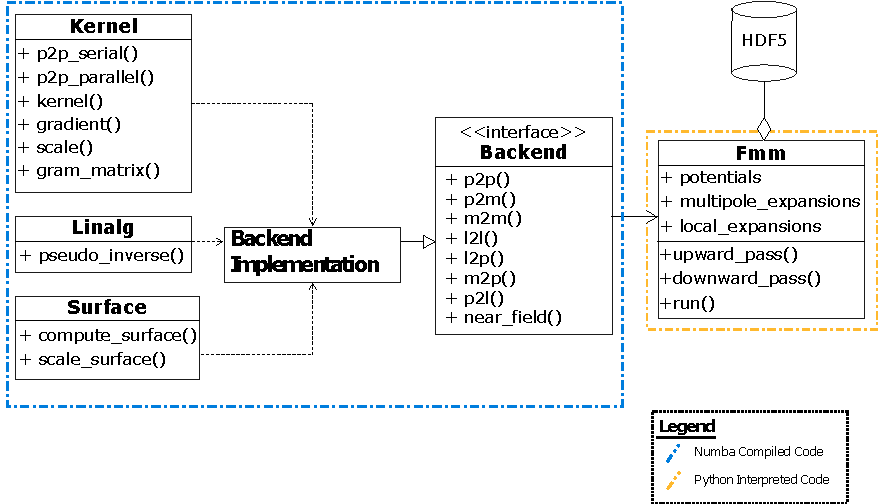
\includegraphics {ch_4/software.pdf}}
    \caption{Simplified UML model of all PyExaFMM components. Trees and other precomputed quantities are stored in a HDF5 database. The `Fmm' object acts as the user interface, all other components are modules consisting of methods operating on arrays, adapted from \cite{kailasa2022pyexafmm}.}
    \label{fig:sec_2_2:design}
\end{figure}

\subsection*{Multithreading in Numba}

Numba enables multithreading via a simple parallel for loop syntax (see listing (\ref{code:sec_2_2:parallel_multithreading})) reminiscent of OpenMP. Internally Numba can use either OpenMP or Intel TBB to generate multithreaded code. We choose OpenMP for PyExaFMM, as it's more suited to functions in which each thread has an approximately similar workload. The threading library can be set via the \lstinline{NUMBA_THREADING_LAYER} environment variable.

Numerical libraries such as NumPy and SciPy implement many of their mathematical operations using multithreaded compiled libraries internally, such as OpenBLAS or IntelMKL. Numba compiled versions of these operations retains this internal multithreading. This leads to \textit{nested parallelism} when combined with a multithreaded region declared with Numba, as in listing (\ref{code:sec_2_2:parallel_multithreading}). This is where a parallel region calls a function with another parallel region inside it. Threads created by the two functions are not coordinated by Numba, and this leads to \textit{oversubscription}, where the number of active threads exceeds the CPU's hardware capacity. Many threads are left idle while the CPU is forced to jump between threads operating on different data. This leads to broken cache locality, and hanging threads threads, stuck waiting for others to finish \cite{malakhov2016python}. We avoid this in PyExaFMM by explicitly setting NumPy operations to be single threaded, via the environment variable \lstinline{OMP_NUM_THREADS=1}, before starting our program. This ensures that the only threads created are those explicitly declared using Numba.


\subsection*{Parallising PyExaFMM}

The $T^{P2M}$, $T^{P2L}$, $T^{M2P}$ and $T^{L2P}$ all rely on the $P2P$ operator, as this computes (\ref{eq:ch_2:two_box_calc}) over their respective sources and targets, and are parallelized over their targets the leaf nodes. For the $T^{L2P}$ operator we encourage cache locality for the $P2P$ step, and keep the data structures passed to Numba as simple as possible, by allocating 1D vectors for the source positions, target positions and the source expansion coefficients, such that all the data required to apply an operator to single target node is adjacent in memory. By storing a vector of `index pointers', that bookend the data corresponding to each target in these 1D vectors, we can form parallel for loops over each target to compute the $P2P$ that encourages cache-locality in the CPU. In order to to this, we have to first iterate through the target nodes, and lookup the associated data to fill the cache local vectors.

The speedup achieved with this strategy, in comparison to a naive parallel iteration over the $T^{L2P}$'s targets, increases with the number of calculations in each thread and hence the expansion order $p$. In an experiment with 32768 leaves, the maximum number of points per leaf, $n_{crit} = 150$, and expansion order $P=10$, our strategy is $13$ \% faster. This corresponds to a realistic FMM problem with approximately $1e6$ randomly distributed particles.

Due to their large interaction lists, the previous strategy is too expensive in terms of memory for the near field, $T^{M2L}$ and $T^{M2P}$ operators. For example, allocating an array large enough to store the maximum possible number of source particle coordinates in double precision for the $T^{M2P}$ operator; with $|W|=148$ and $n_{crit}=150$, requires $\sim 17$GB, and a runtime cost for memory allocations that exceeds the computation time. Instead, for the $T^{M2L}$ we perform a parallel loop over the target nodes at each given level, and over the leaf nodes for the M2P and near field, looking up the relevant data from the linear tree as needed. The $T^{P2L}$ interaction list of each target is at most 19 nodes, and the P2M must also calculate a check potential, cancelling out any speedup from cache locality for these operators.

The matrices involved in the $T^{M2M}$ and $T^{L2L}$ operators can be precomputed and scaled at each level \cite{wang2021exafmm}, and their application is parallelized over all nodes at a given level. Multithreading in this way means that we call the P2P, $T^{P2M}$, $T^{M2P}$, $T^{L2P}$ and near field operators once during the algorithm, the $T^{M2L}$ and $T^{L2L}$ are called $d-2$ times, and the $T^{M2M}$ is called $d$ times, where $d$ is the depth of the octree. This is the minimum number of calls while keeping the operator implementations separate for unit testing.

Figure (\ref{fig:sec_2_2:cpu_wall}) compares the time spent within each Numba-compiled operator (`CPU time') to the total runtime (`wall time') of each operator. The results are computed over five trials over $32768$ leaves, with $n_{crit}=150$ and $P=6$, for a random distribution of $1e6$ charges distributed on the surface of a sphere representing a typical FMM problem. The mean size of the interaction lists are $|U|=11$, $|V|=42$, $|X|=3$, $|W|=3$, and the entire algorithm is computed in $5.95 \pm 0.02 s$, with an additional $9.00 \pm 0.01 s$ for operator pre-computations for a given dataset, which is unachievable in ordinary single-threaded interpreted Python.

The wall time includes the time to (un)box data, organize inputs for Numba compiled functions, and pass control between Numba and Python. Except for the $T^{L2P}$ which has a different parallelization strategy that requires significant data organization that must take place within the GIL restricted Python interpreter, the runtime costs are less than 5 \% of each operator's total wall time, implying that we are nearly always running multithreaded code and utilizing all available CPU cores. 

 \begin{figure}
	\centerline{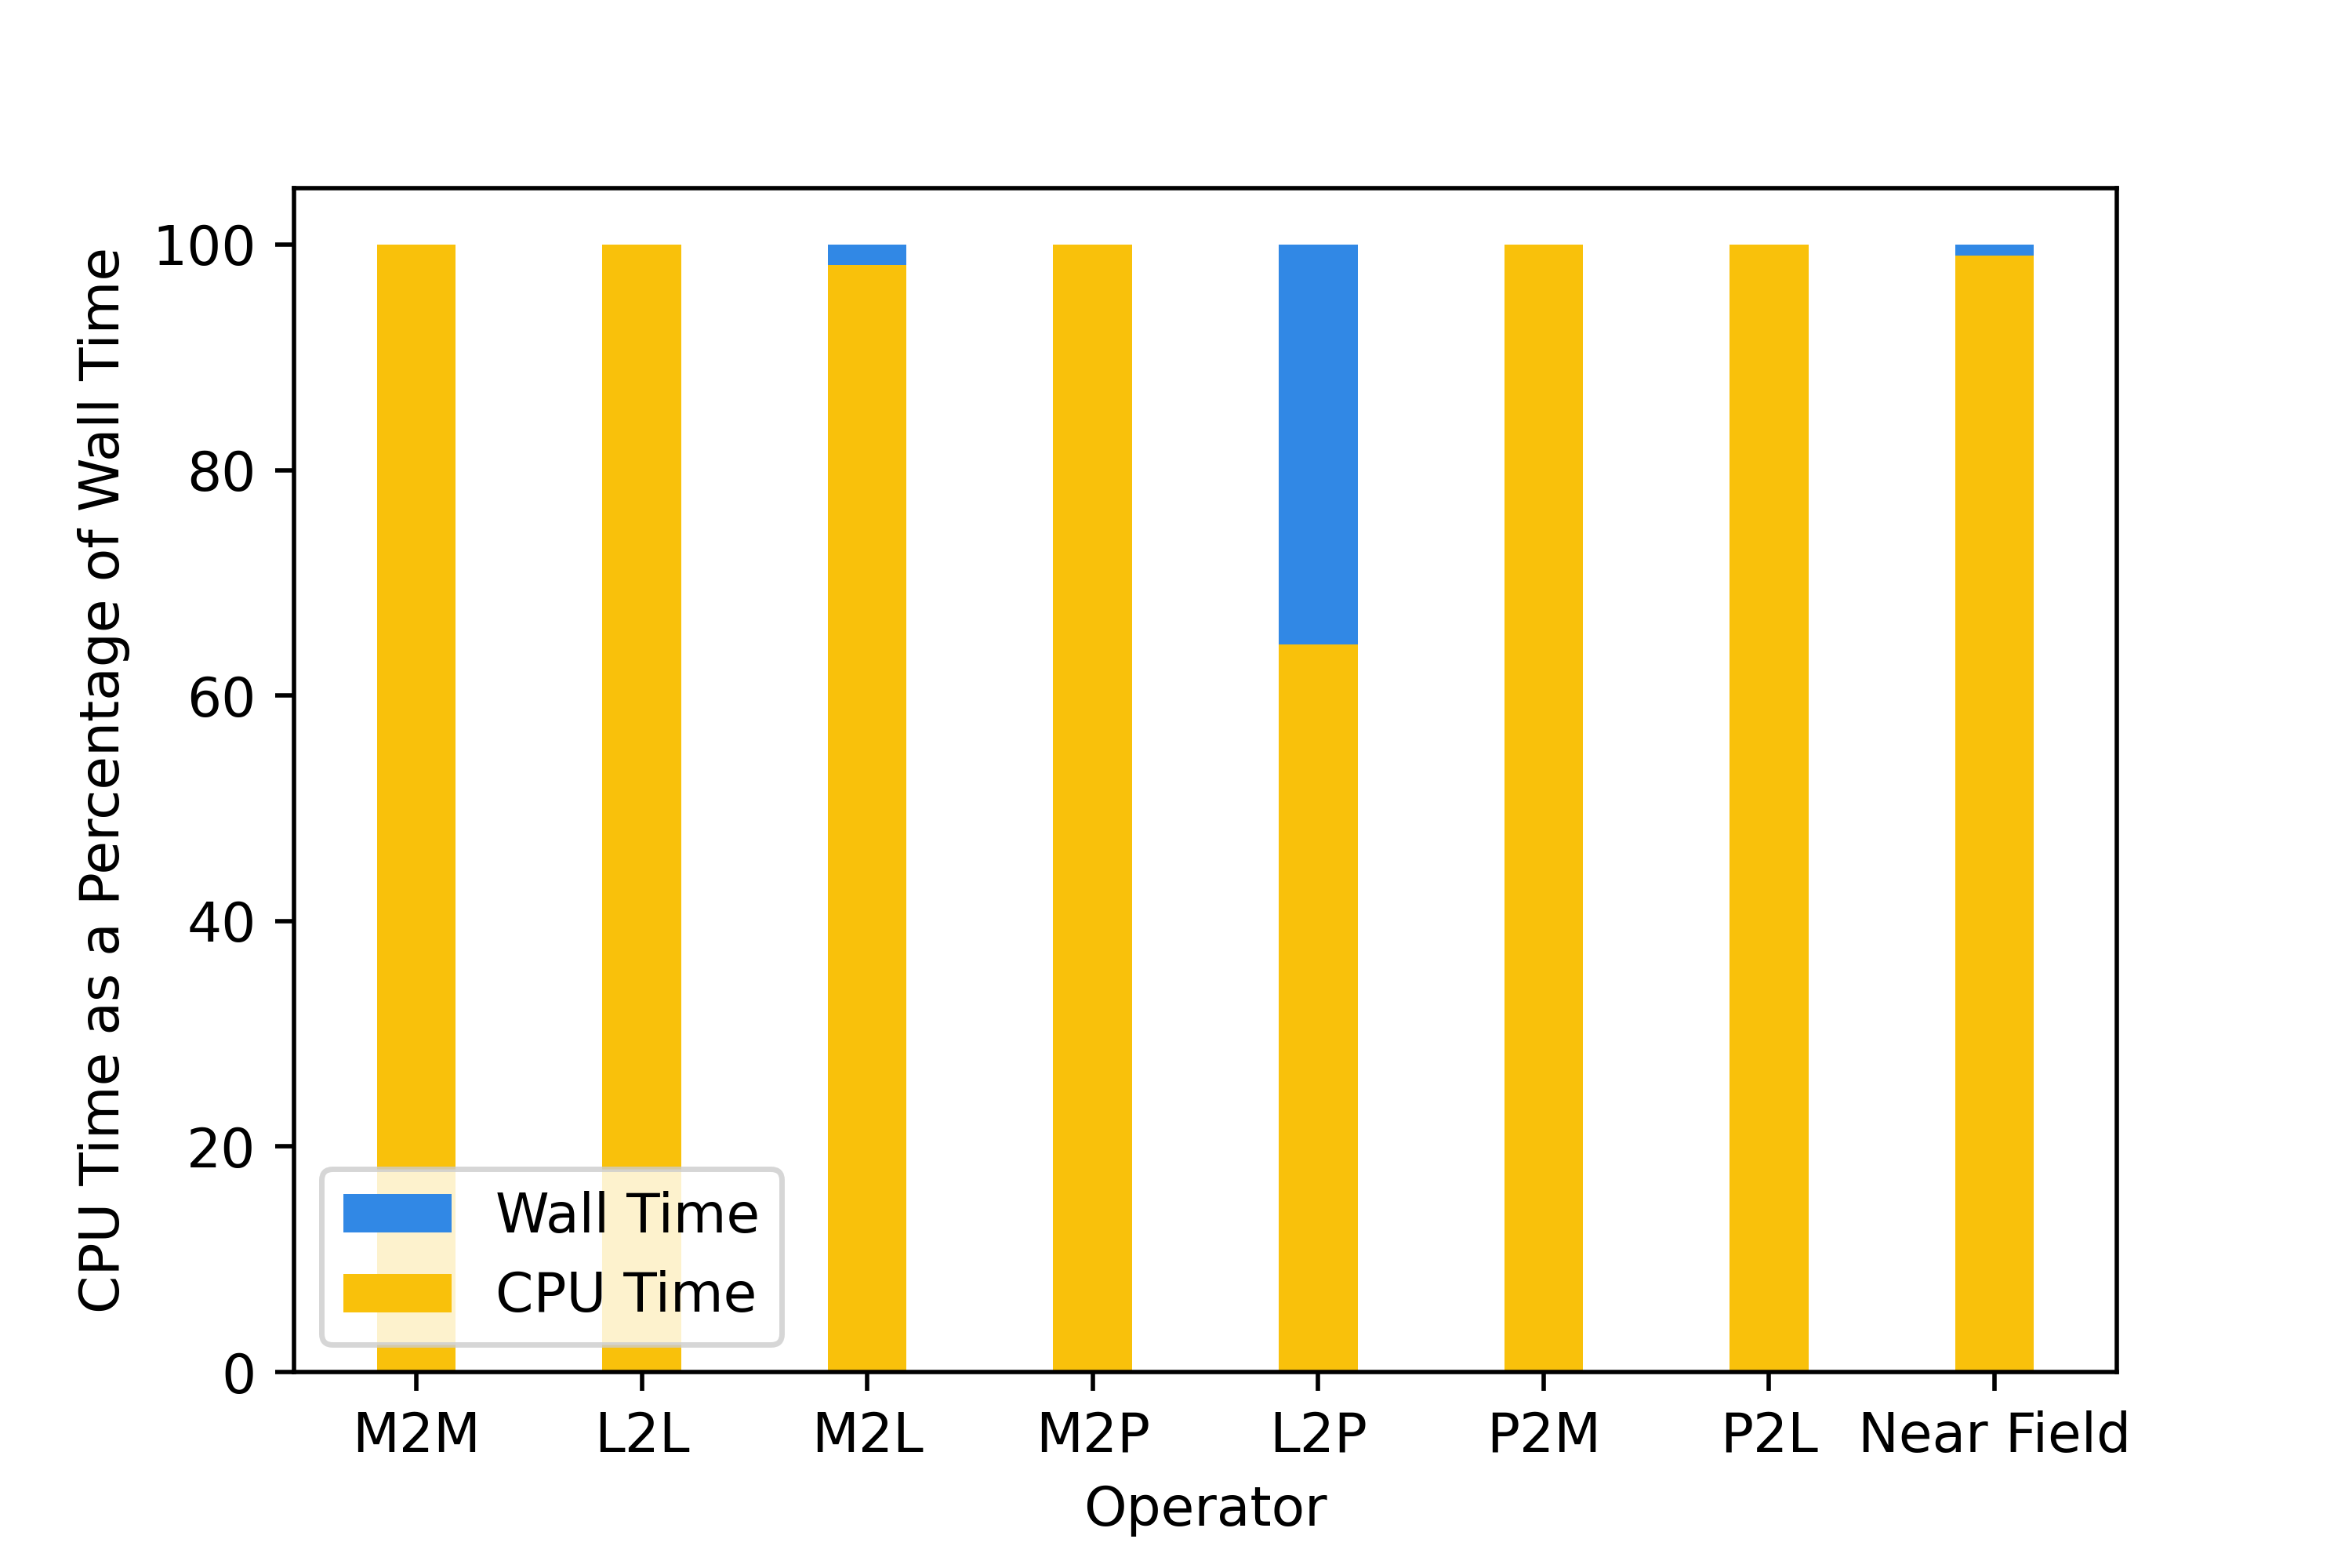
\includegraphics[width=8cm]{ch_4/cpu_wall.png}}
    \caption{CPU time as a percentage of wall time for operators. CPU time is defined as the time in which the algorithm runs pure Numba compiled functions. Wall time is CPU time in addition to the time taken to return control to the Python interpreter, adapted from \cite{kailasa2022pyexafmm}. } 
	\label{fig:sec_2_2:cpu_wall}
\end{figure}


\subsection*{Conclusion}

Achieving optimal multithreaded performance with Numba requires careful consideration of the algorithm being accelerated, details of Numba's backend implementation, as well as a design that suits Numba's data oriented framework. The pitfalls illustrated above show how a user must potentially adapt their code significantly in order to achieve the best performance. Altogether, Numba accelerated code may look decidedly un-Pythonic despite using Python syntax. The complexities involved when using Numba to implement a non-trivial algorithm contrast with its advertisement as a simple way of injecting performance into Python code by applying a decorator. Significant software development expertise is needed in order to optimise a Numba implementation, and arguably more than many in its intended target audience can be expected to possess. 

Despite this, Numba is a remarkable tool. Projects which value Python's expressiveness, simple cross platform builds, as well as large open source ecosystem, and only contain a small number of isolated performance bottlenecks would benefit the most from a Numba implementation. Indeed, by writing only in Python our project size is kept minimal with the entire project running to just 4901 lines of code. Furthermore, we are able to deploy PyExaFMM cross platform trivially with Conda and distribute our software in popular Python channels. 

Resultantly, we wish to find a middle way, that would retain the usability of a higher level language, with the performance benefits of writing in a lower level language, filling the gap from the handoff between a high-level language interface and the programming constraints, as well as the handoff performance hit of a JIT. We believe that this is offered by Rust, which despite being a compiled language, that retains many of these features. 

\begin{figure}
    \centerline{\includegraphics{ch_4/numba.pdf}}
    \caption{Simplified execution path when calling a Numba compiled function from the Python interpreter. The blue path is only taken if the function hasn't been called before. The orange path is taken if a compiled version with the correct type signature already exists in the Numba cache, adapted from \cite{kailasa2022pyexafmm}.}
    \label{fig:sec_2_2:numba_runtime}
\end{figure}

\pythonexternal[basicstyle=\footnotesize, caption={An example of parallel multithreading.}\label{code:sec_2_2:parallel_multithreading}]{snippets/parallel_multithreading.py}
\pythonexternal[basicstyle=\footnotesize, caption={An example of using Numba in a Python function operating on ndarrays.}\label{code:sec_2_2:loop_fusion}]{snippets/loop_fusion.py}

\pythonexternal[basicstyle=\footnotesize,caption={Three ways of writing a trivial algorithm that passes around a vector, while performing some computations.}\label{code:sec_2_2:nested_function}]{snippets/nested_function.py}

    % \chapter{Case Study: Rusty Tree, a Rust Based Parallel Octree}\label{chpt:5}
Interpreted languages, such as Python, Matlab or Julia, offer great usability benefits. They each support large ecosystems of numerical libraries, and offer rapid prototyping due to their interpreted nature. The tools to build software with these languages is designed for portability across a large variety of platforms, from different hardware architectures to operating systems. However, as we have observed in chapter \ref{chpt:4:pyexafmm}, this comes with the overhead of having to deal with an interpreter, and impacts the kind of software that can realistically be built with interpreted languages.

For problems in which this overhead is untenable, compiled languages, such as C, C++ and Fortran are preferred. These languages require greater software engineering expertise, as developers are responsible for allocating memory, installing third party libraries, as well as building their software to target different hardware. These languages in a sense allow a developer to `do anything', of course only if one knows how to do it. The higher software engineering barrier manifests in a dizzying array of compilers, build systems, package managers, testing and documentation libraries and code organisation techniques. The notable thing about all of these optional choices is that it is relatively unclear which is the \textit{preferred} way of doing things, with novice developers likely to find a development strategy that `simply works' and stick to it. Rust stands in contrast to these traditionally preferred compiled languages for high performance scientific computing. Although it is comparably fast it is relatively \textit{inflexible}, with a strongly preferred way of organising, testing, documenting and deploying software. This leads to significantly more uniform Rust code across projects, and a steep, though relatively shorter, learning curve. Importantly, this uniformity makes Rust code easier to share, and port to different operating systems and hardware targets.

\subsection*{Package Managers and Build Systems}

For simple programs, it's tempting to use a compiler directly to create an executable, as in listing (\ref{code:sec_2_3:simple_compilation}). However, as a project's codebase expands, with files defined in multiple directories and calls to external libraries often written in other programming languages, this simple one line appeal to a compiler will no longer be sufficient. One could always download their requisite software, and install globally over the machine using a system package manager, and attempt to recompile. However, this quickly becomes untenable if one is developing for a range of hardware and operating system targets, or one needs to use different versions of external binaries and libraries. Therefore, software is usually constructed using a `build system'. This is catch all term that refers to a program that takes source files as input and produces a deployable set of binaries or libraries as an output. Classically, build systems were based on `Make' and `Autotools', these softwares generate `Makefiles' - which are recipes for constructing a piece of software given a set of source files and external dependencies. These are robust tools, but the onus is squarely with a developer for ensuring that all dependent libraries are visible to Make, and that the external packages are all of compatible versions.

To manage this complexity, builds are often defined using a metabuild system, most commonly CMake. CMake is a scripting language, and as a meta build system it takes a specification of local and third party dependencies and hardware targets, and generates Makefiles. CMake gives developers a great deal of flexibility, it is multi-platform, and language agnostic, however using it directly is not straightforward. Indeed, there is a significant body of literature discussing best practices with CMake \cite{scott2018professional}, however CMake is not responsible for downloading and installing third party packages, or verifying their relative compatibility, implementing its best practices are again left to users.

Approaches for reliable builds vary amongst projects, ranging from `low tech' readme driven solutions, in which a user follows a recipe of instructions, to more modern automated solutions. Figure (\ref{fig:sec_2_3:builds}) provides an overview of the different approaches taken. The lack of a uniform standard means that some projects go as far as to implement a custom build system, such as the Boost library \cite{boostbuild2022github}.

Keeping on top of packages, which are constantly being iterated upon independently, and may support different features with each release, is nearly impossible to do manually. Furthermore, one may want to support a specific set of packages, and respectively versions, for a given hardware or operating system target, but a different set for a different build of the same software. This has led to the development of `package managers' which are a catch all term for softwares that can download and install required software for you, and often verify whether version constraints are satisfied too. Package managers can be delineated into `system package managers', which download operating system specific packages written in any language globally on your machine, and `language specific package managers' which focus only on packages written in a given target language, but are operating system agnostic from a user's perspective.

In terms of system package managers Linux examples include apt, yum and debian, for MacOS there is Homebrew, and Chocolatey for Windows. These can handle both source installations, in which source code is compiled upon download, as well as binary installation, in which pre-built binaries matching your hardware constraints are installed. Binary installation is often preferred, as it is faster, and often reflects a stable release. Language specific package managers, such as pip for Python, which can handle dependencies written in these languages only. Developing your own packages for system package managers is not developer friendly, official package repositories of Linux package managers are moderated by their respective maintainers, though it is possible to set up a personal repository this is quite a sophisticated approach for simple research outputs. The simple alternative, pursued by up to 26 \% of surveyed C++ softwares (see fig. (\ref{fig:sec_2_3:builds})), is to simply add third party software as a submodule. Often to ease installation, C++ libraries are shipped as `header only' libraries, this makes them easy to install, requiring only an \pythoninline{#include}. However by using such techniques a project can quickly grow to contain thousands, to millions of lines of code, much of it in dependencies. Compiling from source has the potential to be a painstakingly slow process, and must be repeated for every combination of hardware and operating system targets one wants to run on.

\begin{figure}
    \centerline{\includegraphics[width=0.95\linewidth]{ch_2/builds.pdf}}
    \caption{An overview of building software in other compiled languages.}
    \label{fig:sec_2_3:builds}
\end{figure}

With the exception of Fortran, which has made recent strides to develop a standardised modern package manager and build system, inspired by Rust's Cargo \cite{fpm2022github}, C and C++ do not have a single officially supported package manager or build system. The resulting landscape is a multitude of package managers \cite{spack2022github, vcpkg2022github, conan2022github} and build systems \cite{meson2022github, bazel2022github, scons2022github} a few of which we have cited here, all of which replicate each others functionality, none of which are universally accepted or implemented across projects nor officially supported by the C++ software foundation.

\bashexternal[basicstyle=\footnotesize, caption={Compiling a simple \texttt{source\_code.cpp} into a \texttt{compiled\_binary} file from a terminal.}\label{code:sec_2_3:simple_compilation}]{simple_compilation.sh}

Recent years have seen the bundling of package managers \textit{with} build systems, resulting in softwares that can simply take source files, and a set of dependencies, and resolve a single binary output for a given hardware and software target. Examples include Conda for Python, and Rust's Cargo system. These modern efforts are able to compile both source and binary packages for all operating systems, and can target a wide range of hardware architectures. Furthermore, the trend has been towards the specification of project dependencies in a single structured text file (see listing (\ref{code:sec_2_3:simple_cargo})), which is then handled by the package manager with no further user effort. Efforts have been in this direction for older compiled languages, the most notable examples being Spack and Conan (see fig. (\ref{fig:sec_2_3:builds})). Importantly, in the case of Rust, Cargo is officially supported and shipped as a core part of its runtime. In contrast to C, C++ and Fortran, Rust has a \textit{single} officially supported compiler, rustc. By taking global decisions for all software written in Rust, a significant burden is removed from developers of Rust software, similar to the situation in many interpreted languages. Indeed Cargo builds are often executed in a \textit{single line}, eradicating the complex readme driven builds common in other compiled languages. For the project specified by listing (\ref{code:sec_2_3:simple_cargo}) can be compiled from a terminal with the command: \texttt{cargo build}.

\bashexternal[basicstyle=\footnotesize, caption={An example of a simple \texttt{Cargo.toml} file for a Rust project, with source as well as binary dependencies.}\label{code:sec_2_3:simple_cargo}]{snippets/Cargo.toml}

\subsection*{Code Organisation and Quality}

Rust introduces many ergonomic features for code organization. The most novel features, which may not be familiar to those coming from other compiled languages, are the concepts of traits, lifetimes and the borrow checker.

\subsubsection*{Traits}

Traits are Rust's system for specifying shared behaviour and building abstraction, constituting a wholesale replacement of object oriented programming, with its inheritance based hierarchies. Traits only enforce \textit{behaviour}, and therefore are strictly less brittle than object orientation which enforces a type. We provide some example syntax in listing (\ref{code:sec_2_3:simple_traits}), and contrast it to equivalent object oriented code in ;listing (\ref{code:sec_2_3:simple_class}). We notice that the object oriented code has a built in hierarchy, which means that adding shared behaviour will effect our \pythoninline{MyType} type, and everything that subsequently depends on it, in contrast to the trait based code in which we can inject new behaviour into MyType, its subsequent dependents we only need to know about the traits and their associated interfaces that they themselves rely on. This means that one can focus solely on the behaviour implicit in a given Trait, rather than having to comb through a potentially complex hierarchy of objects and inheritance to understand what a given line of code is doing, making large Rust projects significantly more readable than their object oriented equivalents.

Traits can be seen to specify shared behaviour in a bottom up manner, as opposed to top down object orientation, new features can be injected into existing types. This is useful for scientific programming, as we are usually concerned with data oriented programming. As we saw in chapter \ref{chpt:3} exploring data oriented programming in Python, object oriented design obfuscates operations on the data itself behind abstraction.

\rustexternal[basicstyle=\footnotesize, caption={An example of a trait implemented on a custom type.}\label{code:sec_2_3:simple_traits}]{snippets/trait.rs}

\pythonexternal[basicstyle=\footnotesize, caption={An example of behaviour in listing (\ref{code:sec_2_3:simple_class}) implemented in an object oriented manner}\label{code:sec_2_3:simple_class}]{snippets/pyclass.py}

This isn't to say similar syntax isn't available in other compiled languages. In C++20, `concepts' were introduced as a trait like mechanism to specify interfaces. However, as with many things in C++, this isn't enforced and it is up to a user to choose to implement their code in this manner. This is borne out in the fact that concepts are \textit{nominally typeed}, and therefore don't enforce behaviour as in Rust's \textit{structurally typed} traits. The implication of this being that a type may `accidentally' implement a concept, if it happens to define its relevant methods. A consequence of this is that a valid C++ program can contain a confusing mix of trait based, and object oriented code, with a a reader then dependent on documentation to understand a software's behaviour, and what has been enforced and where, by the developer.

\subsubsection*{Lifetimes and the Borrow Checker}

Another new Rust concept for developers coming from other compiled languages is the idea of `lifetimes' and `ownership'. Every reference in Rust has an associated lifetime, and a singular `owner'. Which enforce the programming pattern of `resource allocation is initialisation' (RAII) as a feature of the Rust compiler. The basic rule is that references are owned within a scope, and dropped when out of scope. We provide a basic example in listing (\ref{code:sec_2_3:borrowing}), in a Rust context RAII is better encapsulated by another acronym `destructors run at exit scope' (DRES). 

\rustexternal[basicstyle=\footnotesize, caption={A demonstration of basic rules of borrowing and ownership.}\label{code:sec_2_3:borrowing}]{snippets/ownership.rs}

Lifetimes are a Rust concept that guarantees that any references to a resource live at least as long as the resource itself. The main aim of this to prevent dangling references, whereby references to unintended data, or de-allocated data, are not present in the compiled binary. This removes a large class of common bugs from Rust software such as dangling pointers, and double free errors. We illustrate this in listing (\ref{code:sec_2_3:lifetimes}), which won't compile as the inner scope defines a value \pythoninline{x}, which doesn't survive into the outer scope. 

\rustexternal[basicstyle=\footnotesize, caption={A demonstration of lifetimes as a function of scope. This example is adapted from the Cargo book \cite{klabnik2019rust}.}\label{code:sec_2_3:lifetimes}]{snippets/lifetimes.rs}

Rust's compiler enforces ownership and lifetime rules uses a program called the `borrow checker' to ensure that all references, and lifetimes, are referring to valid memory locations at \textit{compile time} without the need for a runtime garbage collector. This is a huge advantage over other compiled languages, for example memory related bugs have been found to constitute as much as 70 \% of all security bugs at Microsoft \cite{microsoft2019}. From a scientific programming perspective, handling memory additionally bogs down algorithm development, iteration, and ultimately publication, and was one of the major contributing factors in the push towards interpreted languages in recent decades. Again, this is not to say similar features do not exist in other compiled languages. C++ has its notion of `smart pointers', which enforce RAII principles too, however as with other features in C++, this is a library feature rather than a core part of its compiler, or language specification, making it optional and unenforced. 

The benefits of Rust's memory system extend to parallel code too. A wide variety of programming paradigms for parallel computation with threads exist, in scientific software we often use OpenMP, which uses the shared memory paradigm, such that all threads operate on the same data. In this setting one of the most common bugs is a data race condition, whereby multiple threads attempt to write to the same memory location. Rust's ownership system enforces the atomicity of all memory operations, by passing ownership between threads, as only a single mutable reference can exist to a piece of memory Rust is able to prevent data races at compile time. Although atomic operations are available in OpenMP, or other shared memory systems, the benefit of Rust is that we know that our compiled code \textit{cannot} contain this bug, without having to rely on unit tests for expected behaviour.

\subsubsection*{Code Quality}

Rust's runtime includes a test runner, a documentation generator, and a code formatter. As with other Rust features, these are maintained in lock step with the language specification, and with reference to other Rust developments. This imposes universal constraints on all Rust projects, allowing for objectively defined `good' Rust code, rather than relying on various standards of best practices that vary between projects and organisations.

\subsection*{Rust's Scientific Ecosystem and Foreign Libraries}

Despite being a young language, Rust already supports a mature ecosystem of libraries for scientific computing with high-level multithreading support \cite{rayon2018github}, numerical data containers \cite{ndarray2022github}, and tools for generating interfaces to Python \cite{maturin2022github}.

Many tools are yet to be ported into native Rust, however high quality bindings exist for core tools such as MPI \cite{rsmpi2018github}, BLAS and LAPACK \cite{blaslapackrust2022github}. The problem with interfacing with tools written in other languages is again related to building software, however Cargo offers tools to build software written in other languages and integrate it with Rust code via the \pythoninline{build} crate, which allows one to leverage existing build systems written for software written in foreign languages. This detracts from the benefits offered by Cargo as a unified package manager and build system, raising similar problems to those encountered when building software in other compiled languages. However, we observe that this remains a concern of the software's developer, who is responsible for providing build scripts for the operating systems and hardware platforms that they wish to support, and from a downstream user perspective their build process remains the same as with pure Rust packages, where the dependency is defined in their \pythoninline{Cargo.toml} file.

We also note that Rust is missing key tools for scientific computing, such as a code generation for GPUs, as well as for advanced optimised advanced linear algebra routines, especially for sparse matrices. However, both of these applications are an active area of development.

\subsection*{Conclusion}

Rust's syntax and program structure are strongly opinionated, its build system emphasises simplicity and portability, and its ecosystem for scientific computing is rapidly developing. A small software team, as is common in academic settings, writing in Rust are effectively able to maintain and deploy Rust projects to a wide variety of platforms, from laptops to supercomputers. Rust's simplified build process results in minimal configuration for users, encouraging the widespread adoption of Rust projects.

    % \chapter{A Fast Direct Solver for Strongly Admissable Problems}\label{chpt:6}
Fast direct solvers constitute a fast-matrix inversion - in contrast to the fast matrix-vector product of the FMM. This section describes ongoing work on the formulation of a new fast direct solver for solving low-medium frequency scattering problems that are described by the Helmholtz equation. This is a part of joint work developed in collaboration with researchers at the Flatiron Institute. 

In section (\ref{sec:1_1_motivation}) we introduced boundary integral equations (\ref{eq:generic_int_equation:sec:1_1}) and their matrix representation (\ref{eq:linear_system:sec:1_1}), noting that it could alternatively be represented using hierarchical matrices. As we have seen, these matrix representations (HSS, $\mathcal{H}^2$ etc.) allow us to rapidly \textit{apply} the system matrix (\ref{eq:linear_system:sec:1_1}) with linear or near linear time complexity. In combination with modern \textit{iterative} methods, such as GMRES \cite{saad1986gmres}, with $O(n_k)$ iterations such that $n_k \ll N$ where $N$ is the number of unknowns in the system, the solution of such problems is brought into practical reach. However, there are situations in which iterative methods fall short. For example for problems which have \textit{multiple} right hand sides we wish to solve for. In such cases, recently developed \textit{fast direct} methods offer a promising alternative. The inversion of a dense linear system by classical direct methods, such as Gaussian Elimination or LU decomposition, have a complexity of $O(N^3)$. Fast direct methods however take advantage of the low-rank structure implicit in the matrix of (\ref{eq:generic_int_equation:sec:1_1}) to find an approximation for the inverse in a similar manner to the FMM. The main trade-off between fast direct methods and the iterative alternative is the relatively greater memory cost in having to pre-compute and store the matrix factorization.

Numerous approaches have been implemented for fast direct solvers for the matrix factorisations described in section (\ref{sec:1_1_motivation}). Here we introduce the `Recursive Strong Skeletonisation' (RS-S) algorithm of Minden et. al \cite{minden2017recursive}, which incorporates strong admissibility and has good properties for parallelisation. Our main contribution is the extension of this technique to effectively handle acoustic scattering problems at low to moderate frequencies where the size of the problem domain is less than a few hundred times the wavelength, building on the exterior Dirichlet case first presented in \cite{sushnikova2022fmm}. 

\subsection*{Problem Formulation}

We start by deriving the boundary integral equation for the boundary value problem described by the Helmholtz equation and an exterior Dirichlet boundary condition,

\begin{flalign}
    \label{eq:sec_3_1:helmholtz_ext_dir}
    (\Delta + k^2) u = 0, \> \> \text{in } \mathbb{R^d} \setminus \Omega \\
    u = f, \> \> \text{on } \Gamma \\ 
    \lim_{r \rightarrow \infty} r \left ( \frac{\partial u}{ \partial r} - iku \right ) = 0
\end{flalign}

The final line above describes a `radiation condition', which is required to maintain the uniqueness of $u$. Physically, the solution $u$ corresponds to the spatial distribution of a wave scattered from an object with domain $\Omega$ and boundary $\Gamma$ embedded in $\mathbb{R}^d$ where without loss of generality we will take $d=3$. 

Using the definition of the free space Green's function,

\begin{flalign}
    \Phi(\mathbf{x}, \mathbf{y}) = \frac{e^{ik|\mathbf{x} -\mathbf{y}|}}{4\pi |\mathbf{x} - \mathbf{y}|}
\end{flalign}

And defining,

\begin{flalign}
    K(\mathbf{x}, \mathbf{y}) = (\mathbf{n}(y) \cdot \nabla_{\mathbf{y}}\Phi(\mathbf{y}, \mathbf{x})) -ik \Phi(\mathbf{x}, \mathbf{y}) 
\end{flalign}

where $n(\mathbf{y})$ is the outwardly facing unit normal at $y \in \partial \Gamma$, we define the \textit{combined field representation} of $u$ as,

\begin{flalign}
    \label{eq:sec_3_1:combined_field_representation}
    u &= \int_\Gamma K(\mathbf{x}, \mathbf{y}) \sigma(\mathbf{y}) da(\mathbf{y}), \> \> \mathbf{x} \in \mathbb{R}^3 \setminus \Omega \\
    &= \int_\Gamma (\mathbf{n}(y) \cdot \nabla_{\mathbf{y}}\Phi(\mathbf{y}, \mathbf{x})) -ik \Phi(\mathbf{x}, \mathbf{y}) \sigma(\mathbf{y}) da(\mathbf{y}) \\
    &= (\mathcal{D} - ik \mathcal{S}) \sigma
\end{flalign}

where we also define the double layer, $\mathcal{D}$, and single layer, $\mathcal{S}$ potential operators. Representing $u$ in terms of layer potentials gives us a solution of the the PDE (\ref{eq:sec_3_1:helmholtz_ext_dir}), however the `surface density' $\sigma$ is unknown. Armed with a representation we can proceed to form a \textit{boundary integral equation} defined only along $\Gamma$ in terms of the the unknown $\sigma$,

\begin{flalign*}
    (\mathcal{D} -ik \mathcal{S} + \frac{1}{2})\sigma(\mathbf{x}) = f(\mathbf{x}), \> \> \mathbf{x} \in \Gamma
\end{flalign*}

Here we have used the well known \textit{jump relations} which describe a discontinuity in the value of the double layer potential operator as we approach the boundary. Further information about layer potentials, the particular benefits of the combined field representation and the jump relations can be found in appendix \ref{app:a_5:bie} For our purposes it's sufficient to recognise that this boundary integral equation motivates our work on fast direct solvers. Writing it in another form,

\begin{flalign}
    \frac{1}{2} \sigma(\mathbf{x}) + \int_\Gamma K(\mathbf{x}, \mathbf{y}) \sigma(\mathbf{y}) da(\mathbf{y}) = f(\mathbf{x})
\end{flalign}

we see that it can be discretised using a suitable method, such as the Galerkin or Nyström methods. Using Nyström we arrive at the following linear system,

\begin{flalign}
    \label{eq:sec_3_1:bie}
    \frac{1}{2} \sigma_i + \sum_{j=1, j \neq i}^N K(\mathbf{x}_i, \mathbf{x}_j) \sigma_j w_{ij} = f(x_i)
\end{flalign}

where $\mathbf{x}_i$ and $w_{ij}$ are the quadrature nodes and weights, respectively, and $\sigma_i$ is the approximation to $\sigma(\mathbf{x}_i)$. Solving this equation for $\sigma$, allows one to find the approximation of the general solution of the scattering problem (\ref{eq:sec_3_1:helmholtz_ext_dir}) in the exterior using (\ref{eq:sec_3_1:combined_field_representation}).

\subsection*{Recursive Strong Skeletonisation}

Consider a domain containing the discretisation points of the boundary $\Gamma$, $\mathbf{x}_i \in \Gamma$. We proceed to discretise with an adaptive, 2:1 balanced, octree. The idea of strong skeletonisation is then to use the \textit{interpolative decomposition} (ID) \cite{cheng2005compression}, a dense matrix compression algorithm, to globally compress matrices with low-rank structure for the case in which only particular off-diagonal blocks are low-rank. In our problem of interest, (\ref{eq:sec_3_1:bie}), where the low-rank assumption only applies when two nodes of an octree are strongly admissible with respect to each other, i.e. the far-field interactions via the kernel of the integral equation.

\begin{definition}[Interpolative Decomposition (ID)]
    Given a matrix $A_{\mathcal{I} \mathcal{J}} \in \mathbb{C}^{|\mathcal{I}| \times |\mathcal{J}|}$ with rows indexed by $\mathcal{I}$ and columns indexed by $|\mathcal{J}$, an $\epsilon$ accurate interpolative decomposition of $A$ is a partitioning of $\mathcal{J}$ into a set of so-called skeleton columns denoted by $\mathcal{S} \subset \mathcal{J}$ and redundant columns $\mathcal{R} = \mathcal{J} \setminus \mathcal{S}$, and the construction of a corresponding interpolation matrix $T$ such that,

    $$\| A_{\mathcal{I} \mathcal{R}} - A_{\mathcal{I} \mathcal{S}} T \| \leq \epsilon \| A_{\mathcal{I} \mathcal{J}} \| $$

    Where we take the norms to be defined as the standard spectral norm. The interpretation of the above is that the redundant columns are well approximated by a linear combination of the skeleton columns. We compute the ID using a column-pivoted QR decomposition as in \cite{sushnikova2022fmm}, which has a complexity of $O(|\mathcal{I}| \cdot |\mathcal{J}|^2)$.
    \label{def:sec_3_1:id}
\end{definition}

Now we consider a three by three block matrix, $A \in \mathbb{C}^{N \times N}$, taking a partition of the index set such that $[N]= \mathcal{I} \cup \mathcal{J} \cup \mathcal{K}$ with $[N] = {1, 2, ... N}$ such that $A_{\mathcal{I} \mathcal{K}} = 0 = A_{\mathcal{K} \mathcal{I}}$,

\begin{flalign*}
    A = \begin{bmatrix}
        A_{\mathcal{I} \mathcal{I}} & A_{\mathcal{I} \mathcal{J}} & 0 \\
        A_{\mathcal{J} \mathcal{I}} & A_{\mathcal{J} \mathcal{J}} & A_{\mathcal{J} \mathcal{K}} \\
        0 & A_{\mathcal{K} \mathcal{J}} & A_{\mathcal{K} \mathcal{K}}
    \end{bmatrix}
\end{flalign*}

Assuming $A_{\mathcal{I} \mathcal{I}}$ is invertible, and using block Gaussian elimination we can decouple this block from the rest of the matrix as follows,

\begin{flalign*}
    L \cdot A \cdot U = \begin{bmatrix}
        I & 0 & 0 \\
        - A_{\mathcal{J} \mathcal{I}} A_{\mathcal{I} \mathcal{I}}^-1 & I & 0 \\
        0 & 0 & I 
    \end{bmatrix} \cdot A \cdot \begin{bmatrix}
        I - A_{\mathcal{I} \mathcal{I}}^-1 A_{\mathcal{I} \mathcal{J}} & 0 \\
    0 & I & 0 \\
    0 & 0 & I
    \end{bmatrix} = \begin{bmatrix}
        A_{\mathcal{I} \mathcal{I}} & 0 & 0 \\
        0 & S_{\mathcal{J} \mathcal{J}} &  A_{\mathcal{J} \mathcal{K}} \\
        0 &  A_{\mathcal{K} \mathcal{J}} &  A_{\mathcal{K} \mathcal{K}}
    \end{bmatrix}
\end{flalign*}

where the block $S_{\mathcal{J} \mathcal{J}} = A_{\mathcal{J} \mathcal{J}} - A_{\mathcal{J} \mathcal{I}}A_{\mathcal{I} \mathcal{I}}^-1A_{\mathcal{I} \mathcal{J}}$ is the only non-zero block that has been modified, with the second term in $S_{\mathcal{J} \mathcal{J}}$ is known as the Schur complement update.

We now attempt to apply this decoupling to the matrix, $A$, that arises from our boundary integral formulation. Taking $\mathcal{B}$ as the set of indices of points $x_i$ contained in box $B$ in the octree, $\mathcal{N}$ as the indices of the points in $B$'s near field and $\mathcal{F}$ as the points contained in its far field, as defined by the strong admissibility condition, upon appropriate permutation by a matrix $P$ we arrive at the following block structure for $A$.

\begin{flalign}
    \label{eq:sec_3_1:decomp_a}
    P^TAP = \begin{bmatrix}
        A_{\mathcal{B} \mathcal{B}} & A_{\mathcal{B} \mathcal{N}} & A_{\mathcal{B} \mathcal{F}} \\ 
        A_{\mathcal{N} \mathcal{B}} & A_{\mathcal{N} \mathcal{N}} & A_{\mathcal{N} \mathcal{F}} \\ 
        A_{\mathcal{F} \mathcal{B}} & A_{\mathcal{F} \mathcal{N}} & A_{\mathcal{F} \mathcal{F}}
    \end{bmatrix}
\end{flalign}

We want to numerically compress the far-field interactions, i.e. the blocks corresponding to $A_{\mathcal{B} \mathcal{F}}$ and $A_{\mathcal{F} \mathcal{B}}$ using the ID, as they are considered to be numerically low-rank. To do so, we decouple into a set of redundant points, denoted by indices $\mathcal{R}$ and skeleton points, denoted by indices $\mathcal{S}$, such that (up to a permutation) we have,

\begin{flalign*}
    \begin{bmatrix}
        A_{\mathcal{F} \mathcal{B}} \\ 
        A_{\mathcal{B} \mathcal{F}}^T
    \end{bmatrix} = \begin{bmatrix}
        A_{\mathcal{F} \mathcal{R}} & A_{\mathcal{F} \mathcal{S}} \\
        A_{\mathcal{R} \mathcal{F}}^T & A_{\mathcal{R} \mathcal{S}}^T
    \end{bmatrix} \approx \begin{bmatrix}
        A_{\mathcal{F} \mathcal{S}} \\
        A_{\mathcal{S} \mathcal{F}}
    \end{bmatrix}^T \cdot \begin{bmatrix}
        T & I
    \end{bmatrix}
\end{flalign*}

where we've applied the ID as an approximation. We've applied the same $T$ interpolation matrix for both blocks, making the assumption that the kernel is symmetric. The authors in \cite{sushnikova2022fmm} note that this in practice can also be done for non-symmetric kernels, at the cost of a small increase in the number of skeleton points. 

Returning to (\ref{eq:sec_3_1:decomp_a}), and further splitting $\mathcal{B} = \mathcal{R} \cup \mathcal{S}$ and applying the previous approximation for the far-field blocks, we get

\begin{flalign*}
    P^T A P = \begin{bmatrix}
        A_{\mathcal{R} \mathcal{R}} & A_{\mathcal{R} \mathcal{S}}  & A_{\mathcal{R} \mathcal{N}} & A_{\mathcal{R} \mathcal{F}} \\  
        A_{\mathcal{S} \mathcal{R}} & A_{\mathcal{S} \mathcal{S}}  & A_{\mathcal{S} \mathcal{N}} & A_{\mathcal{S} \mathcal{F}} \\ 
        A_{\mathcal{N} \mathcal{R}} & A_{\mathcal{N} \mathcal{S}}  & A_{\mathcal{N} \mathcal{N}} & A_{\mathcal{N} \mathcal{F}} \\ 
        A_{\mathcal{F} \mathcal{R}} & A_{\mathcal{F} \mathcal{S}}  & A_{\mathcal{F} \mathcal{N}} & A_{\mathcal{F} \mathcal{F}}  
    \end{bmatrix} = \begin{bmatrix}
        A_{\mathcal{R} \mathcal{R}} & A_{\mathcal{R} \mathcal{S}}  & A_{\mathcal{R} \mathcal{N}} & T^TA_{\mathcal{S} \mathcal{F}} \\  
        A_{\mathcal{S} \mathcal{R}} & A_{\mathcal{S} \mathcal{S}}  & A_{\mathcal{S} \mathcal{N}} & A_{\mathcal{S} \mathcal{F}} \\ 
        A_{\mathcal{N} \mathcal{R}} & A_{\mathcal{N} \mathcal{S}}  & A_{\mathcal{N} \mathcal{N}} & A_{\mathcal{N} \mathcal{F}} \\ 
        A_{\mathcal{F} \mathcal{S}}T & A_{\mathcal{F} \mathcal{S}}  & A_{\mathcal{F} \mathcal{N}} & A_{\mathcal{F} \mathcal{F}}   
    \end{bmatrix}
\end{flalign*}

As the redundant rows and columns of interactions between the points in $\mathcal{R}$ and $\mathcal{F}$ are well approximated by the interactions between $\mathcal{S}$ and $\mathcal{F}$ we can decouple these points from the rest of the problem as follows. Let $E$ and $F$ be `elimination' matrices defined on a partition $[N] = \mathcal{R} \cup \mathcal{S} \cup \mathcal{N} \cup \mathcal{F}$ as,

\begin{flalign*}
    E = \begin{bmatrix}
        I & -T^T & & \\
        & I & & \\ 
        & & I & \\
        & &  & I \\
    \end{bmatrix} \text{ and } F = \begin{bmatrix}
        I & & & \\
        -T & I & & \\ 
        & & I & \\
        & &  & I \\ 
    \end{bmatrix}
\end{flalign*}

Then,

\begin{flalign*} 
    EP^T A P F = \begin{bmatrix}
        X_{\mathcal{R} \mathcal{R}} &X_{\mathcal{R} \mathcal{S}}  & X_{\mathcal{R} \mathcal{N}} & 0 \\  
        X_{\mathcal{S} \mathcal{R}} & A_{\mathcal{S} \mathcal{S}}  & A_{\mathcal{S} \mathcal{N}} & A_{\mathcal{S} \mathcal{F}} \\ 
        X_{\mathcal{N} \mathcal{R}} & A_{\mathcal{N} \mathcal{S}}  & A_{\mathcal{N} \mathcal{N}} & A_{\mathcal{N} \mathcal{F}} \\ 
        0 & A_{\mathcal{F} \mathcal{S}}  & A_{\mathcal{F} \mathcal{N}} & A_{\mathcal{F} \mathcal{F}}  
    \end{bmatrix}
\end{flalign*}

where $X_{\mathcal{I} \mathcal{J}}$ indicates blocks which have been updated in comparison to the original matrix. Assuming that $X_{\mathcal{R} \mathcal{R}}$ is invertible, we can use it as a pivot block to decouple the redundant degrees of freedon. Let $L$ and $U$ be defined as,

\begin{flalign*}
    L = \begin{bmatrix}
        I &  & & \\
        -X_{\mathcal{S} \mathcal{R}} X_{\mathcal{R} \mathcal{R}}^{-1}& I & & \\ 
        -X_{\mathcal{N} \mathcal{R}} X_{\mathcal{R} \mathcal{R}}^{-1}& & I & \\
        & &  & I \\
    \end{bmatrix} \text{ and } U = \begin{bmatrix}
        I &  - X_{\mathcal{R} \mathcal{R}}^{-1} X_{\mathcal{R} \mathcal{S}} & - X_{\mathcal{R} \mathcal{R}}^{-1} X_{\mathcal{R} \mathcal{N}}  & \\
         & I & & \\ 
        & & I & \\
        & &  & I \\ 
    \end{bmatrix}
\end{flalign*}

Then 

\begin{flalign*}
    Z(A; B) &= LEP^T A PFU \\
    &= \begin{bmatrix}
        X_{\mathcal{R} \mathcal{R}} & 0 & 0 & 0 \\
        0 &  X_{\mathcal{S} \mathcal{S}}& X_{\mathcal{S} \mathcal{N}} & A_{\mathcal{S} \mathcal{F}} \\ 
        0 &  X_{\mathcal{N} \mathcal{S}}& X_{\mathcal{N} \mathcal{N}} & A_{\mathcal{N} \mathcal{F}}  \\
        0 &  A_{\mathcal{F} \mathcal{S}}& A_{\mathcal{F} \mathcal{N}} & A_{\mathcal{F} \mathcal{F}}  
    \end{bmatrix}
\end{flalign*}

This matrix is of the previous decoupled form for a generic matrix. This decoupling is referred to as the \textit{strong skeletonisation} of $A$ with respect to $B$, with the resulting matrix denoted with $Z(A;B)$. Therefore we can write $A$ in terms of a block LU-style factorisation,

\begin{flalign*}
    A = (PE^{-1}L^{-1})Z(A;B)(U^{-1}F^{-1}P^T) = V Z(A;B) W
\end{flalign*}

where $V$ and $W$ are called the skeletonisation operators, which can be stored and used in factored form. Moreover $L$ $U$ $E$ and $F$ are block triangular, with identities in their diagonal and thus are trivial to invert. Giving us a compact representation for skeletonisation,

\begin{flalign*}
    Z(A;B) = V^{-1} A W^{-1}
\end{flalign*}

The recursive strong skeletonisation (RS-S) proceeds by sequentially applying strong skeletonisation to each box in an octree that describes the points on arising from the discretisation of the boundary integral equation. The boxes in the tree are traversed in an upward pass, similar the FMM. After each application of the strong skeletonisation only the skeleton points $S$ associated with each box are retained, referred to as `active degrees of freedom'. For boxes at coarser levels the active degrees of freedom are constructed from the active degrees of freedom of its children, at which point strong skeletonisation is applied again. The process continues until there are no active degrees of freedom for any box in a given box's far field - which is true by definition at level 1 of the tree. Denoting the skeletonisation operators of box $i$ as $V_i$ and $W_i$, and assuming the algorithm terminates at box $B_M$, we denote the permutation matrix $P_t$ which orders the remaining active degrees of freedom in $B_M's$ domain, denoted with $\mathcal{B}_t$. This results in a final RS-S factorisation of $A$ as,

\begin{flalign*}
    A \approx (V_1 V_2 \dots V_M) P_t D P_t^T (W_M W_{M-1} \dots W_1)
\end{flalign*}

where $D$ is a block diagonal matrix given by,

\begin{flalign*}
    D = \begin{bmatrix}
        X_{\mathcal{R}_1\mathcal{R}_1} & &  & \\
        & \ddots &  &  \\
        & &  X_{\mathcal{R}_M\mathcal{R}_M} & \\
        & & & A_{\mathcal{B}_t\mathcal{B}_t}
    \end{bmatrix}
\end{flalign*}

Using this decomposition we can rapidly compute $A^{-1}$, and hence our `fast direct solve' with,

\begin{flalign*}
    A^{-1} \approx (W_1^{-1} \dots W_M^{-1}) P_t D^{-1}P_t^T (V_M^{-1} \dots V_1^{-1})
\end{flalign*}

\subsection*{The Proxy Trick}

The complexity of the fast direct solver described by the RS-S technique is determined by the cost of computing the ID for the far-field interactions of a given box in the octree, $B$. This will in general contain $O(N)$ points. Therefore computing the ID with respect to far field interactions as we've done above will scale as $O(N^2)$ for each box. The authors of \cite{minden2017recursive} employ the so called `proxy trick' to reduce this complexity, and recover an $O(N)$ scaling for their fast direct solver. Our contribution in this work is the explicit formulation of the proxy trick for a variety of integral equation kernels that appear in scattering problems, with specific application to  acoustic scattering problems.

The main idea of the proxy trick rests on the principle of representing the far-field particles of a given box $B$, which may contain $O(N)$ particles, with a set of `proxy points' contained on a proxy surface that encloses $B$. This surface is often chosen to be a sphere. By choosing $O(1)$ proxy points, without getting into the details yet of how exactly they are sampled, we are able to obtain the linear complexity we desire.

For a given box $B$, a proxy surface $D$ and its boundary $\gamma$ are chosen such that $B \subset D$. The far-field points of $B$, $\mathcal{F}$ is partitioned such that $\mathcal{F} = \mathcal{Q} \cup \mathcal{P}$, where $\mathcal{Q}$ contains $O(1)$ points. $\Gamma$ is the boundary of the entire scatterer, and $\tau = \Gamma \cap B$ is the portion of the scatterer boundary contained in $B$. The situation is sketched in figure (\ref{fig:sec_3_1:proxy_trick}) in 2D.

\begin{figure}
    \centering
    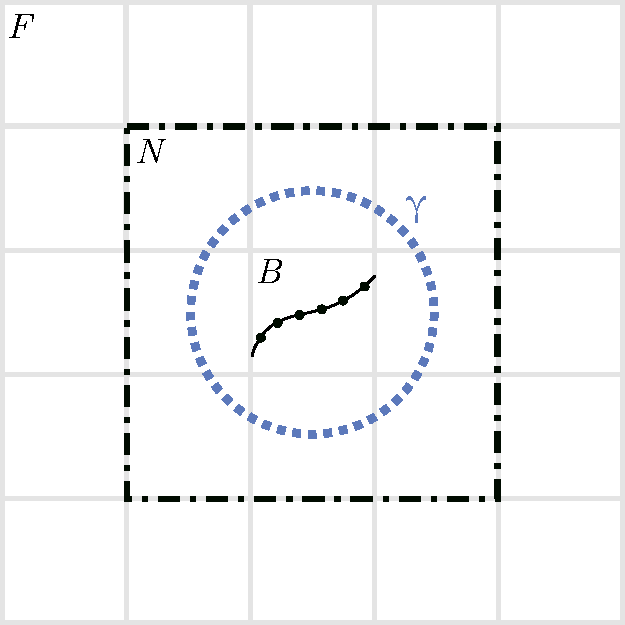
\includegraphics[width=0.5\textwidth]{ch_3/proxy.pdf}
    \caption{Considering the outgoing problem due to charge contained on $\Gamma \cap B$ evaluated in the far-field of $B$ in $\mathbb{R}^2$.}
    \label{fig:sec_3_1:proxy_trick}
\end{figure}

We can choose to represent our solution due to the charge in $B$ in $\mathcal{F}$ however we wish. However, our choice will lead to different matrices that we must compress.

Generally, we'll end up with a solution matrix of the form $A_{\mathcal{F}B}$ that maps between the charge contained $B$, $\psi_B$, and potential, $v_\mathcal{F}$, at points in its far-field that can be split up as,

\begin{flalign}
    v_{\mathcal{F}} &= A_{\mathcal{F}B} \psi_B \\
    &= B_{\mathcal{F}\gamma} C_{\gamma B} \psi_B
\end{flalign}

the subscripts indicate the domains these operators map between. We desire a split like this as the far field interaction of $B$ can be expressed as an object involving $C_{\gamma B}$ only.

To see how such a split can be useful consider the fact that $A_{\mathcal{F}B}$ can be written as,

\begin{flalign}
    \label{eq:decomposition}
    A_{\mathcal{F}B} = \begin{bmatrix}
        A_{\mathcal{Q}B}\\ A_{\mathcal{P}B}
        \end{bmatrix} = \begin{bmatrix}
        I & 0\\ 0 & B_{\mathcal{P}\gamma}
        \end{bmatrix} \begin{bmatrix}
        A_{\mathcal{Q}B}\\ C_{\gamma B}
        \end{bmatrix}
\end{flalign}

Our RS-S algorithm relies on a compression of this matrix, however as we noted a direct compression of $A_{\mathcal{F} B}$ is too expensive. However if we can find a decomposition like above, we can apply an interpolative decomposition to the right column in (\ref{eq:decomposition}) which has dimensions $O(1) \times O(n_\gamma)$ by construction where $n_\gamma$ is the number of proxy points. To prove that this allows us to reconstruct the full matrix after compression. Consider an ID that gives us,

\begin{flalign}
    \begin{bmatrix}
        A_{\mathcal{Q}B}\\ C_{\gamma B}
        \end{bmatrix} = \begin{bmatrix}
            A_{\mathcal{Q}S}\\ C_{\gamma S}
        \end{bmatrix} \begin{bmatrix}T_{SR}  & 1 \end{bmatrix}
\end{flalign}

Where $S$ and $R$ are the skeleton and redundant points respectively. Plugging back into our expression (\ref{eq:decomposition}),

\begin{flalign}
    \label{eq:compressed}
    A_{\mathcal{F}B} &=
        \begin{bmatrix}
            I & 0\\ 0 & B_{\mathcal{P}\gamma}
        \end{bmatrix}
        \begin{bmatrix}
             A_{\mathcal{Q}S}\\ C_{\gamma S}
        \end{bmatrix}
        \begin{bmatrix}T_{SR}  & 1 \end{bmatrix} \\
        &=\begin{bmatrix}
            A_{\mathcal{Q}S}\\ B_{\mathcal{P} \gamma}C_{\gamma S}
       \end{bmatrix} \begin{bmatrix}T_{SR}  & 1 \end{bmatrix} \\
       &=  A_{\mathcal{F}S} \begin{bmatrix}T_{SR}  & 1 \end{bmatrix}
\end{flalign}

Therefore, we see that we can get away with a cheap ID to reconstruct the far-field operator, involving the proxy points rather than the full far field of $B$. We are thus left with the task of formulating the proxy trick to compress the correct components of the boundary integral kernel.

Below we consider how to apply the proxy trick for different representations of the far-field potential due to the charges contained in $B$, known as `outgoing skeletonisations', as well the inverse operation in which the proxy trick is applied to calculate the potentials within $B$ due to charges in its far-field, known as `incoming skeletonisations'.

\subsubsection*{Hypersingular - $\mathcal{T}$}

\subsubsection*{Outgoing Skeletonisation}

A double-layer potential, due to some unknown density $\psi$, supported on $\tau$,

\begin{flalign}
    v(x) = \int_{\Gamma \cap B} \frac{\partial \Phi(x, y)}{\partial n(y)} \psi(y) ds(y) := \mathcal{D}\psi, \> \> x \in \mathbb{R}^m \setminus \tau
\end{flalign}

solves the Helmholtz equation everywhere it's valid. Here, $\Phi(x, y)$ is the fundamental solution of the Helmholtz equation. However, its normal derivative evaluated at the target points, known as the hypersingular operator, which we'll need for deriving boundary integral equations for Maxwell problems, does not,

\begin{flalign}
    \frac{\partial v}{\partial n(x)} = \frac{\partial}{\partial n(x)} \int_{\Gamma \cap B} \frac{\partial \Phi(x, y)}{\partial n(y)} \psi(y)ds(y) := \mathcal{T}\psi, \> \> x \in \Gamma \cap \mathcal{F}
\end{flalign}

it's only valid at far-field points, $\Gamma \cap \mathcal{F}$. However, we can separate out the normal part of the derivative,

\begin{flalign}
    \frac{\partial v}{\partial n(x)} = n(x) \cdot \nabla_x \int_{\Gamma \cap B} \frac{\partial \Phi(x, y)}{\partial n(y)} \psi(y)ds(y) := n \cdot w
\end{flalign}

The function

\begin{flalign}
    w(x) = \nabla_x \int_{\Gamma \cap B} \frac{\partial \Phi(x, y)}{\partial n(y)} \psi(y)ds(y) := \nabla_x \mathcal{D}\psi
\end{flalign}

Does satisfy our PDE, everywhere, and we'll exploit this fact in a moment. As an aside, we can see that this is true by considering a double layer potential $v$ that is smooth enough to admit,

\begin{flalign}
    (\Delta + k^2)w =(\Delta + k^2)\nabla_x v =\nabla_x (\Delta + k^2) v = 0
\end{flalign}

where the last equality follows as $v$ satisfies the Helmholtz equation. Therefore $w$ is a solution of the Helmholtz equation. Note that $w$ has three components.

In order to find our $C_{\gamma B}$ with this representation, we need to set up an `associated boundary value problem' for each component of $w$. The choice of boundary value problem we choose is free, as we only rely on the existence of its solution.

Consider an associated boundary value problem for just a single component of $\tilde{w}$ that satisfies,

\begin{flalign}
    &(\Delta + k^2)\tilde{w} = 0, \> \> x \in \mathbb{R}^m \setminus D \\
    &\tilde{w} = w_1(x) \\
    &\text{A radiation condition at } \infty
\end{flalign}

A combined field representation might be nice, as we know it has good properties,

\begin{flalign}
    \tilde{w} = (\mathcal{D} - ik \mathcal{S})_{\mathcal{F}\gamma} \mu
\end{flalign}

where $\mu$ is some unknown density supported on the proxy surface $\gamma$. Forming the boundary integral equation, and plugging back into the representation for $\tilde{w}$,

\begin{flalign}
    \tilde{w} &=  (\mathcal{D} - ik \mathcal{S})_{\mathcal{F} \gamma}(\frac{1}{2}\mathcal{I} + \mathcal{D} - ik \mathcal{S})_{\gamma \gamma}^{-1}w_1 \\
    &= (\mathcal{D} - ik \mathcal{S})_{\mathcal{F} \gamma}(\frac{1}{2}\mathcal{I} + \mathcal{D} - ik \mathcal{S})_{\gamma \gamma}^{-1} \nabla_1 \mathcal{D}_{\gamma B} \psi_\gamma \\
    &\equiv B_{\mathcal{F}\gamma} C_{\gamma B} \psi_\gamma
\end{flalign}

where we identify,

\begin{flalign}
    C_{\gamma B} = \nabla_1 \mathcal{D}_{\gamma B}
\end{flalign}

This is the matrix we will attempt to compress. Similar analysis follows for the other two components of $w(x)$. Meaning that we end up having to compress $[\nabla_1 \mathcal{D}_{\gamma B} , \nabla_2 \mathcal{D}_{\gamma B} , \nabla_3 \mathcal{D}_{\gamma B}]$ for the outgoing problem. We note that $B_{\mathcal{F} \gamma }$ is never explicitly formed, we just require its existence. When we calculate an approximation of $A_{\mathcal{F}B}$ using (\ref{eq:compressed}), we only need to know the ID of the $C_{\gamma B}$.

\subsubsection*{Incoming Skeletonisation}

For the incoming skeletonization, were again we're considering the same representation with a hypersingular operator, we observe that we're just looking for,

\begin{flalign}
    \left [\frac{\partial v}{\partial n(x)} \right ]_{\mathcal{F} B}^T
\end{flalign}

with the formation of an associated boundary integral equation taking place in much the same way as for the outgoing problem. However, the hypersingular operator is self-adjoint, therefore it leads to the same expressions for $C_{\gamma B}$.

\subsubsection*{Derivative of the Single Layer - $\mathcal{K}'$}

\subsubsection*{Outgoing Skeletonisation}

If we choose to represent our potential with a single-layer potential,

\begin{flalign}
    u(x) = \int_{\Gamma \cap B} \Phi(x, y) \phi(y) ds(y) := \mathcal{S}\phi, \> \> x \in \mathbb{R}^m \setminus \tau
\end{flalign}

and seek a boundary integral equation in terms of its normal derivative at the targets,

\begin{flalign}
    w(x) = \int_{\Gamma \cap B} \frac{\partial \Phi(x, y)}{\partial n(x)} \phi(y) ds(y) := \mathcal{K}'\phi, \> \> x \in \Gamma \cap \mathcal{F}
\end{flalign}

We observe the same problem as in the $\mathcal{T}$ case, where this expression is not a general solution of our PDE. We can similarly separate out the normal component and write,

\begin{flalign}
    \tilde{w}(x) := \int_{\Gamma \cap B} \nabla_x \Phi(x, y) \phi(y) ds(y), \> \> x \in \mathbb{R}^m \setminus \tau
\end{flalign}

Using the previous analysis for $\mathcal{T}$, we immediately recognise that the components we must compress are $C_{\gamma B} = \nabla_1 \mathcal{S}_{\gamma B}$, giving us $[\nabla_1 \mathcal{S}_{\gamma B}, \nabla_2 \mathcal{S}_{\gamma B}, \nabla_3 \mathcal{S}_{\gamma B}]$ to compress in total for the outgoing problem.

\subsubsection*{Incoming Skeletonisation}

Noticing that,

\begin{flalign}
    \left [\frac{\partial u}{\partial n(x)} \right ]_{\mathcal{F} B}^T = \int_{\Gamma \cap B} \frac{\partial \Phi(x, y)}{\partial n(y)} \phi(y) ds(y) = \mathcal{D}_{\gamma B} \phi
\end{flalign}

already satisfies our PDE without any further work, we can simply use it as our Dirichlet data in the associated boundary value problem. The matrix to compress being $C_{\gamma B} = \mathcal{D}_{\gamma B}$.

\subsubsection*{Single Layer - $\mathcal{S}$}

\subsubsection*{Outgoing Skeletonisation}

We now choose to represent our scattered solution with a single-layer operator,

\begin{flalign}
    u(x) =\int_{\Gamma \cap B} \Phi(x, y)\phi(y)ds(y) := \mathcal{S}\phi,\> \> x \in \mathbb{R}^m \setminus \tau
\end{flalign}

This satisfies the underlying PDE everywhere. We can now set up an associated exterior boundary value problem as before, and use our single-layer potential as Dirichlet boundary data.

\begin{flalign}
    (\Delta + k^2)w= 0, \> \> x \in \mathbb{R}^m \setminus D \\
    w = \mathcal{S}\phi, \> \> \text{on } \gamma \\
    \text{Radiation condition at }\infty
\end{flalign}

where $\phi$ is some unknown density supported on $\tau$. As before, we can form a boundary integral equation for this associated problem, and solve, recognising that the matrix to compress $C_{\gamma B} = \mathcal{S}_{\gamma B}$

\subsubsection*{Incoming Skeletonisation}

The single-layer operator is self-adjoint, leading to the same operator to compress. Spelling this out, consider the associated interior boundary value problem,

\begin{flalign}
    (\Delta + k^2)w= 0\> \> \text{in } D \\
    w = \mathcal{S}\phi \> \> \text{on } \gamma
\end{flalign}

The solution of an interior Helmholtz scattering problem may not be unique, but this doesn't matter for our purposes. Proxy compression doesn't require uniqueness, only existence. Let's seek a solution in the form of a combined-layer potential,

\begin{flalign}
    w(x) = (\mathcal{D}_\gamma - ik \mathcal{S}_\gamma)[\phi](x)
\end{flalign}

where the subscripts make it clear that the density is supported on $\gamma$. Forming the boundary integral equation,

\begin{flalign}
    (-\frac{\mathcal{I}}{2} + \mathcal{D}_\gamma - ik \mathcal{S}_\gamma)[\phi](x) = \mathcal{S}_{\mathcal{F} \gamma}[\phi](x)
\end{flalign}

Solving with the representation gives,

\begin{flalign}
    w = \mathcal{S}_{B \gamma}(-\frac{\mathcal{I}}{2} + \mathcal{D}_\gamma - ik \mathcal{S}_\gamma)^{-1}\mathcal{S}_{\gamma \mathcal{F}}[\phi](x) = C_{B \gamma}B_{\gamma \mathcal{F}}
\end{flalign}

where we recognize the matrix to compress as $C_{B\gamma} = \mathcal{S}_{B\gamma}$ in our proxy framework.

\subsection*{Double Layer - $\mathcal{D}$}

\subsubsection*{Outgoing Skeletonisation}

A double-layer potential, due to some unknown density $\psi$, supported on $\tau$,

\begin{flalign}
    v(x) = \int_{\Gamma \cap B} \frac{\partial \Phi(x, y)}{\partial n(y)} \psi(y) ds(y) := \mathcal{D}\psi, \> \> x \in \mathbb{R}^m \setminus \tau
\end{flalign}

solves the Helmholtz equation everywhere it's valid. Therefore it can be used as Dirichlet data for the associated boundary value problem for the outgoing skeletonization. Applying similar analysis to above, we identify the kernel to compress as $C_{\gamma B} = \mathcal{D}_{\gamma B}$.

\subsubsection*{Incoming Skeletonisation}

We notice that the transpose of the double layer operator is,

\begin{flalign}
    [u]^T_{\mathcal{F}B}(x) = \int_{\Gamma \cap B} \frac{\partial \Phi(x,y)}{\partial n(x)}\phi(y)ds(y)= \mathcal{K}'_{\gamma B}\phi
\end{flalign}

This in general does not satisfy our PDE everywhere, we again separate out the normal component, and as before, recognise that the components to compress are $[\nabla_1 \mathcal{S}_{\gamma B}, \nabla_2 \mathcal{S}_{\gamma B}, \nabla_2 \mathcal{S}_{\gamma B}]$.

\subsection*{Acoustic Sound Hard Scattering}

Let's now apply our fast direct solver framework, with proxy compression to some example problems. We begin with acoustic sound-hard scattering, which is a didactic example. Consider a scattered field $u^s$, that scatters off an object $\Omega$ and satisfies the Helmholtz equation in the exterior,

\begin{flalign}
    (\Delta + k^2)u^s = 0, \> \> \> \text{in  } \mathbb{R}^3 \setminus \Omega
\end{flalign}

The `sound hard' boundary condition on the surfae $\Gamma$ is
\begin{flalign}
    \frac{\partial u^s}{\partial n} = \frac{\partial u^{i}}{\partial n}, \> \> \> \text{in  } \Gamma
\end{flalign}

where $u^i$ is the incident wave. Using the analysis in \cite{Bruno2012}, we write down a `regularised' representation formula for our solution. This regularisation can be shown to have better spectral properties.

\begin{flalign}
    u^s =(\mathcal{K}_k \circ \mathcal{S}_K - i\eta \mathcal{S}_k)
\end{flalign}

where $k$ and $K$ are complex wave numbers, that may not be the same. We can take the trace of this representation, and its normal derivative at the targets, and find a boundary integral equation for the exterior problem,

\begin{flalign}
    (\frac{i \eta}{2} \mathcal{I}- i \eta \mathcal{K}'_k + \mathcal{T}_k \circ \mathcal{S}_K )\mu = g
\end{flalign}

using the Calder\'{o}n identity,

\begin{flalign}
    \mathcal{T}_k\circ \mathcal{S}_k = -\frac{1}{4}\mathcal{I} + \mathcal({K}_k')^2
\end{flalign}

which is true for any $k$, we arrive at a boundary integral equation,

\begin{flalign}
    \left ( i \eta(\frac{1}{2}\mathcal{I}  - \mathcal{K}'_k) - \frac{1}{4}I+ \mathcal({K}_k')^2 \right ) \mu = g
\end{flalign}

by defining $\theta := \mathcal{K}'_k \mu$, we can write the boundary integral equation as a system,

\begin{flalign}
\begin{pmatrix}
(\frac{i\eta}{2} - \frac{1}{4})\mathcal{I} - i \eta \mathcal{K}'_k & \mathcal{K}'_k  \\
 \mathcal{K}'_k & - \mathcal{I}
\end{pmatrix}
\begin{pmatrix} \mu \\ \theta \end{pmatrix} = \begin{pmatrix}
    g \\ 0
\end{pmatrix}
\end{flalign}

We can then place this system into our fast direct solver framework. Despite not knowing how to compress the system matrix altogether, we do know how to compress each block, as they each correspond to displacements of $\mathcal{K}'_k$.

Consider writing out our block matrix as,


\begin{flalign}
    \begin{pmatrix}
        A & B \\ C & D
    \end{pmatrix}
    \begin{pmatrix}
        \mu\\\theta
    \end{pmatrix}
   = \begin{pmatrix}
        g\\ 0
    \end{pmatrix}
\end{flalign}

and re-writing as,

\begin{flalign}
    \begin{pmatrix}
        \begin{pmatrix}
            A_{11} & B_{11} \\ C_{11} & D_{11}
        \end{pmatrix} & . & .\\
        . & . & \\
        . & &     \begin{pmatrix}
            A_{NN} & B_{NN} \\ C_{NN} & D_{NN}
        \end{pmatrix}
    \end{pmatrix}
    \begin{pmatrix}
        \mu_1 \\ \theta_1 \\ . \\ . \\ \mu_n \\ \theta_n
    \end{pmatrix} =
    \begin{pmatrix}
        g_1 \\ 0 \\ . \\ . \\ g_N \\ 0
    \end{pmatrix}
\end{flalign}

This system matrix remains numerically low-rank, and therefore can fit into our RS-S framework. Indeed, we now have to compress a system of matrix operators in order to capture its row space via the proxy trick.

\subsection*{Preliminary Numerical Experiments}

The paper on which we base our work \cite{sushnikova2022fmm} builds on the original RS-S algorithm \cite{minden2017recursive} by:

\begin{enumerate}
    \item Implementing generalized Gaussian quadratures for computing near-field interactions \cite{bremer2013numerical}.
    \item Determining a properly sampled discretisation of the proxy surface which depends on the box size in the octree, so as to sufficiently sample oscillatory kernels without oversampling.
    \item Handling the construction of the far-field partition into $\mathcal{F} = \mathcal{Q} \cup \mathcal{P}$
\end{enumerate}

We defer to to the original paper for a discussion of these aspects \cite{sushnikova2022fmm}. For our simulations we use these algorithms and quadrature rules as a black box in as implemented by the FMM3D-BIE software \cite{fmm3dbie}. To demonstrate the accuracy of the solver in light of our proxy trick formulation, we suppose that the sound hard condition is generated from a set of 50 test points placed at random locations on the surface of a test geometry, for which we choose the `wiggly torus' displayed in figure (\ref{fig:octree_example:sec_1_2}). The results of our solve are then compared to the potential expected from using a combined field representation at 50 random test locations in the exterior of the geometry.

\begin{flalign*}
    \text{error} = \frac{\sqrt{\sum_{j=1}^{50}|\tilde{u}(t_j)-u(t_j)|^2}}{\sqrt{\int_\Gamma|\sigma(x)|^2 da(x)}}
\end{flalign*}

where $\tilde{u}$ is our approximated potential, $u$ is the exact potential calculated from our test points, $t_j$, and $\sigma$ is the calculated charge density from the boundary integral equation. The torus is taken to be in a bounding box, each dimension of which is fixed at $1 \lambda$ where $\lambda$ is the wavelength of the incident wave, and we fix the error of the ID at $\epsilon = 5 \times 10^{-7}$, and the wavenumber $k=0.97$. Experiments are taken on a single-node of the Rusty Cluster at the Flatiron Institute, which consists of 240 28-core Intel Broadwell nodes with 512GB of RAM.

\begin{table}[h!]
    \centering
    \begin{tabular}{||c c c c c c c c||} 
        \hline
        $p$ & $N_{patch}$ & $N$  & $t_f$ (s) & $t_s$ (s)  & $t_q$ (s) & $m_f$ (GB) & $\epsilon$ \\ [0.5ex]
        \hline\hline
        4 & 50  & 750  & 0.8 & 0.03 & 0.8 & 0.04 & $4.7 \times 10^{-3}$ \\
        4 & 200 & 3000 & 6.6 & 0.08 & 1.4 & 0.6  & $3.3 \times 10^{-4}$ \\
        4 & 450 & 6750 & 84.9 & 0.2 & 2.5 & 2.9 & $5.2 \times 10^{-5}$ \\
        4 & 800 & 12000 & 324.9 & 0.6 & 4.2 & 7.5 & $1.6 \times 10^{-5}$ \\
        4 & 1250 & 18750 & 1138.8 & 1.1 & 6.2 & 15.2 & $5.8 \times 10^{-6}$ \\
        4 & 1800 & 27000 & 1839.7 & 1.7 & 8.8 & 25.2 & $2.4 \times 10^{-6}$ \\
        4 & 2450 & 36750 & 3322.6 & 2.4 & 11.8 & 41.1 & $1.2 \times 10^{-6}$ \\
        \hline
    \end{tabular}
    \caption{We measure the $L^2$ error with respect to the density  ($\epsilon$), time for solution ($t_s$), factorisation ($t_f$), quadrature computation ($t_q$) and memory required for factorisation ($m_f$) as a function of quadrature expansion order ($p$) and number of patches used to discretise the geometry ($N_{patch}$).}
    \label{table:sec_3_2:sh}
\end{table}


From table (\ref{table:sec_3_2:sh}), we observe linear scaling for $t_f$. However we observe sub-linear scaling for for $m_f$ and $t_s$, the authors of \cite{sushnikova2022fmm} suggest that this is due to the fixed wavenumber for increasing $N$. Meaning that the additional degrees of freedom introduced beyond a certain sampling in points per wavelength are more easily compressed. In order to make further observations about the convergence rate of our method more data is required, for higher order quadratures. We note that amount of memory used, even for the modest problem sizes tested, can be quite considerable. With our experiment where the number of quadrature points $N=36750$ consuming over 40GB of memory. This demonstrates the main trade-off of fast direct solvers in comparisons to iterative solvers.

\subsection*{Exposing Parallelism}

The RS-S algorithm exposes natural parallelism. Consider figure (\ref{fig:sec_3_1:rss_parallel}) which shows a four-colouring for a non-adaptive octree in $\mathbb{R}^2$ for simplicity, each colour can be independently skeletonised as skeletonisation only updates matrix entries corresponding to a box's near field. The same logic can be applied to the adaptive case, as well as the $\mathbb{R}^3$ case, albeit with more colours. As of writing there are no parallel implementations of the RS-S algorithms available as open-source packages.

\begin{figure}
    \centering
    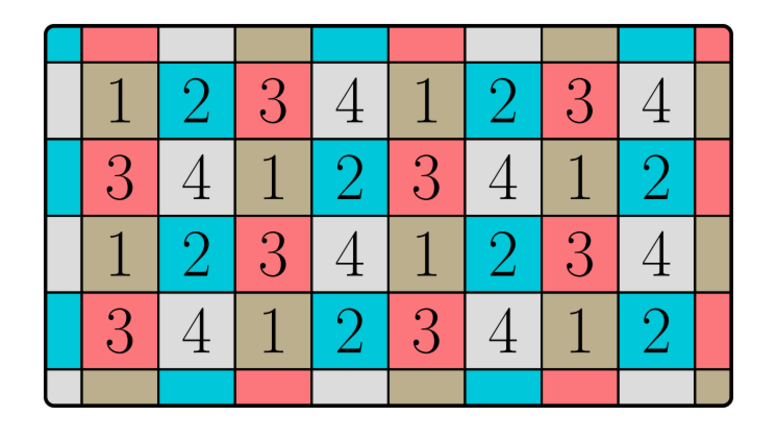
\includegraphics[width=0.5\textwidth]{ch_3/rss-parallel.pdf}
    \caption{A four-colouring of a non-adaptive quadtree in $\mathbb{R}^2$, where the colouring is chosen such that no box shares a colour with its neighbours. All boxes of a given colour can then be skeletonised independently. This figure is adapted from \cite{minden2017recursive}.}
    \label{fig:sec_3_1:rss_parallel}
\end{figure}

\subsection*{Conclusion}

We've described a scalar fast direct solver for solving acoustic scattering problems. We've demonstrated the convergence and scaling of our method with some preliminary numerical results, however further numerical testing is required to study the solvers properties. Specifically to understand its convergence behaviour, and scaling behaviour with higher order quadratures. We have only done cursory work on investigating the effect of quadrature choice, as well as the method chosen for sampling the proxy surface, using the default generalized Gaussian quadratures and sampling techniques described in \cite{sushnikova2022fmm}. This is another potential vector of research. The extension of this solver, and proxy formulation, to the full vectorial case which would allow us to tackle electromagnetic scattering problems as described by Maxwell's equations is an ongoing are of investigation.
    % \chapter{A Fast Direct Solver for Strongly Admissable Problems}\label{chpt:7:fds}
Fast direct solvers constitute a fast-matrix inversion - in contrast to the fast matrix-vector product of the FMM. This section describes ongoing work on the formulation of a new fast direct solver for solving low-medium frequency scattering problems that are described by the Helmholtz equation. This is a part of joint work developed in collaboration with researchers at the Flatiron Institute. 

In chapter \ref{chpt:1:motivation} we introduced boundary integral equations (\ref{eq:generic_int_equation:sec:1_1}) and their matrix representation (\ref{eq:linear_system:sec:1_1}), noting that it could alternatively be represented using hierarchical matrices. As we have seen, these matrix representations (HSS, $\mathcal{H}^2$ etc.) allow us to rapidly \textit{apply} the system matrix (\ref{eq:linear_system:sec:1_1}) with linear or near linear time complexity. In combination with modern \textit{iterative} methods, such as GMRES \cite{saad1986gmres}, with $O(n_k)$ iterations such that $n_k \ll N$ where $N$ is the number of unknowns in the system, the solution of such problems is brought into practical reach. However, there are situations in which iterative methods fall short. For example for problems which have \textit{multiple} right hand sides we wish to solve for. In such cases, recently developed \textit{fast direct} methods offer a promising alternative. The inversion of a dense linear system by classical direct methods, such as Gaussian Elimination or LU decomposition, have a complexity of $O(N^3)$. Fast direct methods however take advantage of the low-rank structure implicit in the matrix of (\ref{eq:generic_int_equation:sec:1_1}) to find an approximation for the inverse in a similar manner to the FMM. The main trade-off between fast direct methods and the iterative alternative is the relatively greater memory cost in having to pre-compute and store the matrix factorization.

Numerous approaches have been implemented for fast direct solvers for the matrix factorisations described in chapter \ref{chpt:2:fmms}. Here we introduce the `Recursive Strong Skeletonisation' (RS-S) algorithm of Minden et. al \cite{minden2017recursive}, which incorporates strong admissibility and has good properties for parallelisation. Our main contribution is the extension of this technique to effectively handle acoustic scattering problems at low to moderate frequencies where the size of the problem domain is less than a few hundred times the wavelength, building on the exterior Dirichlet case first presented in \cite{sushnikova2022fmm}. 

\subsection*{Problem Formulation}

We start by deriving the boundary integral equation for the boundary value problem described by the Helmholtz equation and an exterior Dirichlet boundary condition,

\begin{flalign}
    \label{eq:sec_3_1:helmholtz_ext_dir}
    (\Delta + k^2) u = 0, \> \> \text{in } \mathbb{R^d} \setminus \Omega \\
    u = f, \> \> \text{on } \Gamma \\ 
    \lim_{r \rightarrow \infty} r \left ( \frac{\partial u}{ \partial r} - iku \right ) = 0
\end{flalign}

The final line above describes a `radiation condition', which is required to maintain the uniqueness of $u$. Physically, the solution $u$ corresponds to the spatial distribution of a wave scattered from an object with domain $\Omega$ and boundary $\Gamma$ embedded in $\mathbb{R}^d$ where without loss of generality we will take $d=3$. 

Using the definition of the free space Green's function,

\begin{flalign}
    \Phi(\mathbf{x}, \mathbf{y}) = \frac{e^{ik|\mathbf{x} -\mathbf{y}|}}{4\pi |\mathbf{x} - \mathbf{y}|}
\end{flalign}

And defining,

\begin{flalign}
    K(\mathbf{x}, \mathbf{y}) = (\mathbf{n}(y) \cdot \nabla_{\mathbf{y}}\Phi(\mathbf{y}, \mathbf{x})) -ik \Phi(\mathbf{x}, \mathbf{y}) 
\end{flalign}

where $n(\mathbf{y})$ is the outwardly facing unit normal at $y \in \partial \Gamma$, we define the \textit{combined field representation} of $u$ as,

\begin{flalign}
    \label{eq:sec_3_1:combined_field_representation}
    u &= \int_\Gamma K(\mathbf{x}, \mathbf{y}) \sigma(\mathbf{y}) da(\mathbf{y}), \> \> \mathbf{x} \in \mathbb{R}^3 \setminus \Omega \\
    &= \int_\Gamma (\mathbf{n}(y) \cdot \nabla_{\mathbf{y}}\Phi(\mathbf{y}, \mathbf{x})) -ik \Phi(\mathbf{x}, \mathbf{y}) \sigma(\mathbf{y}) da(\mathbf{y}) \\
    &= (\mathcal{D} - ik \mathcal{S}) \sigma
\end{flalign}

where we also define the double layer, $\mathcal{D}$, and single layer, $\mathcal{S}$ potential operators. Representing $u$ in terms of layer potentials gives us a solution of the the PDE (\ref{eq:sec_3_1:helmholtz_ext_dir}), however the `surface density' $\sigma$ is unknown. Armed with a representation we can proceed to form a \textit{boundary integral equation} defined only along $\Gamma$ in terms of the the unknown $\sigma$,

\begin{flalign*}
    (\mathcal{D} -ik \mathcal{S} + \frac{1}{2})\sigma(\mathbf{x}) = f(\mathbf{x}), \> \> \mathbf{x} \in \Gamma
\end{flalign*}

Here we have used the well known \textit{jump relations} which describe a discontinuity in the value of the double layer potential operator as we approach the boundary. Further information about layer potentials, the particular benefits of the combined field representation and the jump relations can be found in appendix \ref{app:a_5:bie} For our purposes it's sufficient to recognise that this boundary integral equation motivates our work on fast direct solvers. Writing it in another form,

\begin{flalign}
    \frac{1}{2} \sigma(\mathbf{x}) + \int_\Gamma K(\mathbf{x}, \mathbf{y}) \sigma(\mathbf{y}) da(\mathbf{y}) = f(\mathbf{x})
\end{flalign}

we see that it can be discretised using a suitable method, such as the Galerkin or Nyström methods. Using Nyström we arrive at the following linear system,

\begin{flalign}
    \label{eq:sec_3_1:bie}
    \frac{1}{2} \sigma_i + \sum_{j=1, j \neq i}^N K(\mathbf{x}_i, \mathbf{x}_j) \sigma_j w_{ij} = f(x_i)
\end{flalign}

where $\mathbf{x}_i$ and $w_{ij}$ are the quadrature nodes and weights, respectively, and $\sigma_i$ is the approximation to $\sigma(\mathbf{x}_i)$. Solving this equation for $\sigma$, allows one to find the approximation of the general solution of the scattering problem (\ref{eq:sec_3_1:helmholtz_ext_dir}) in the exterior using (\ref{eq:sec_3_1:combined_field_representation}).

\subsection*{Recursive Strong Skeletonisation}

Consider a domain containing the discretisation points of the boundary $\Gamma$, $\mathbf{x}_i \in \Gamma$. We proceed to discretise with an adaptive, 2:1 balanced, octree. The idea of strong skeletonisation is then to use the \textit{interpolative decomposition} (ID) \cite{cheng2005compression}, a dense matrix compression algorithm, to globally compress matrices with low-rank structure for the case in which only particular off-diagonal blocks are low-rank. In our problem of interest, (\ref{eq:sec_3_1:bie}), where the low-rank assumption only applies when two nodes of an octree are strongly admissible with respect to each other, i.e. the far-field interactions via the kernel of the integral equation.

\begin{definition}[Interpolative Decomposition (ID)]
    Given a matrix $A_{\mathcal{I} \mathcal{J}} \in \mathbb{C}^{|\mathcal{I}| \times |\mathcal{J}|}$ with rows indexed by $\mathcal{I}$ and columns indexed by $|\mathcal{J}$, an $\epsilon$ accurate interpolative decomposition of $A$ is a partitioning of $\mathcal{J}$ into a set of so-called skeleton columns denoted by $\mathcal{S} \subset \mathcal{J}$ and redundant columns $\mathcal{R} = \mathcal{J} \setminus \mathcal{S}$, and the construction of a corresponding interpolation matrix $T$ such that,

    $$\| A_{\mathcal{I} \mathcal{R}} - A_{\mathcal{I} \mathcal{S}} T \| \leq \epsilon \| A_{\mathcal{I} \mathcal{J}} \| $$

    Where we take the norms to be defined as the standard spectral norm. The interpretation of the above is that the redundant columns are well approximated by a linear combination of the skeleton columns. We compute the ID using a column-pivoted QR decomposition as in \cite{sushnikova2022fmm}, which has a complexity of $O(|\mathcal{I}| \cdot |\mathcal{J}|^2)$.
    \label{def:sec_3_1:id}
\end{definition}

Now we consider a three by three block matrix, $A \in \mathbb{C}^{N \times N}$, taking a partition of the index set such that $[N]= \mathcal{I} \cup \mathcal{J} \cup \mathcal{K}$ with $[N] = {1, 2, ... N}$ such that $A_{\mathcal{I} \mathcal{K}} = 0 = A_{\mathcal{K} \mathcal{I}}$,

\begin{flalign*}
    A = \begin{bmatrix}
        A_{\mathcal{I} \mathcal{I}} & A_{\mathcal{I} \mathcal{J}} & 0 \\
        A_{\mathcal{J} \mathcal{I}} & A_{\mathcal{J} \mathcal{J}} & A_{\mathcal{J} \mathcal{K}} \\
        0 & A_{\mathcal{K} \mathcal{J}} & A_{\mathcal{K} \mathcal{K}}
    \end{bmatrix}
\end{flalign*}

Assuming $A_{\mathcal{I} \mathcal{I}}$ is invertible, and using block Gaussian elimination we can decouple this block from the rest of the matrix as follows,

\begin{flalign*}
    L \cdot A \cdot U = \begin{bmatrix}
        I & 0 & 0 \\
        - A_{\mathcal{J} \mathcal{I}} A_{\mathcal{I} \mathcal{I}}^-1 & I & 0 \\
        0 & 0 & I 
    \end{bmatrix} \cdot A \cdot \begin{bmatrix}
        I - A_{\mathcal{I} \mathcal{I}}^-1 A_{\mathcal{I} \mathcal{J}} & 0 \\
    0 & I & 0 \\
    0 & 0 & I
    \end{bmatrix} = \begin{bmatrix}
        A_{\mathcal{I} \mathcal{I}} & 0 & 0 \\
        0 & S_{\mathcal{J} \mathcal{J}} &  A_{\mathcal{J} \mathcal{K}} \\
        0 &  A_{\mathcal{K} \mathcal{J}} &  A_{\mathcal{K} \mathcal{K}}
    \end{bmatrix}
\end{flalign*}

where the block $S_{\mathcal{J} \mathcal{J}} = A_{\mathcal{J} \mathcal{J}} - A_{\mathcal{J} \mathcal{I}}A_{\mathcal{I} \mathcal{I}}^-1A_{\mathcal{I} \mathcal{J}}$ is the only non-zero block that has been modified, with the second term in $S_{\mathcal{J} \mathcal{J}}$ is known as the Schur complement update.

We now attempt to apply this decoupling to the matrix, $A$, that arises from our boundary integral formulation. Taking $\mathcal{B}$ as the set of indices of points $x_i$ contained in box $B$ in the octree, $\mathcal{N}$ as the indices of the points in $B$'s near field and $\mathcal{F}$ as the points contained in its far field, as defined by the strong admissibility condition, upon appropriate permutation by a matrix $P$ we arrive at the following block structure for $A$.

\begin{flalign}
    \label{eq:sec_3_1:decomp_a}
    P^TAP = \begin{bmatrix}
        A_{\mathcal{B} \mathcal{B}} & A_{\mathcal{B} \mathcal{N}} & A_{\mathcal{B} \mathcal{F}} \\ 
        A_{\mathcal{N} \mathcal{B}} & A_{\mathcal{N} \mathcal{N}} & A_{\mathcal{N} \mathcal{F}} \\ 
        A_{\mathcal{F} \mathcal{B}} & A_{\mathcal{F} \mathcal{N}} & A_{\mathcal{F} \mathcal{F}}
    \end{bmatrix}
\end{flalign}

We want to numerically compress the far-field interactions, i.e. the blocks corresponding to $A_{\mathcal{B} \mathcal{F}}$ and $A_{\mathcal{F} \mathcal{B}}$ using the ID, as they are considered to be numerically low-rank. To do so, we decouple into a set of redundant points, denoted by indices $\mathcal{R}$ and skeleton points, denoted by indices $\mathcal{S}$, such that (up to a permutation) we have,

\begin{flalign*}
    \begin{bmatrix}
        A_{\mathcal{F} \mathcal{B}} \\ 
        A_{\mathcal{B} \mathcal{F}}^T
    \end{bmatrix} = \begin{bmatrix}
        A_{\mathcal{F} \mathcal{R}} & A_{\mathcal{F} \mathcal{S}} \\
        A_{\mathcal{R} \mathcal{F}}^T & A_{\mathcal{R} \mathcal{S}}^T
    \end{bmatrix} \approx \begin{bmatrix}
        A_{\mathcal{F} \mathcal{S}} \\
        A_{\mathcal{S} \mathcal{F}}
    \end{bmatrix}^T \cdot \begin{bmatrix}
        T & I
    \end{bmatrix}
\end{flalign*}

where we've applied the ID as an approximation. We've applied the same $T$ interpolation matrix for both blocks, making the assumption that the kernel is symmetric. The authors in \cite{sushnikova2022fmm} note that this in practice can also be done for non-symmetric kernels, at the cost of a small increase in the number of skeleton points. 

Returning to (\ref{eq:sec_3_1:decomp_a}), and further splitting $\mathcal{B} = \mathcal{R} \cup \mathcal{S}$ and applying the previous approximation for the far-field blocks, we get

\begin{flalign*}
    P^T A P = \begin{bmatrix}
        A_{\mathcal{R} \mathcal{R}} & A_{\mathcal{R} \mathcal{S}}  & A_{\mathcal{R} \mathcal{N}} & A_{\mathcal{R} \mathcal{F}} \\  
        A_{\mathcal{S} \mathcal{R}} & A_{\mathcal{S} \mathcal{S}}  & A_{\mathcal{S} \mathcal{N}} & A_{\mathcal{S} \mathcal{F}} \\ 
        A_{\mathcal{N} \mathcal{R}} & A_{\mathcal{N} \mathcal{S}}  & A_{\mathcal{N} \mathcal{N}} & A_{\mathcal{N} \mathcal{F}} \\ 
        A_{\mathcal{F} \mathcal{R}} & A_{\mathcal{F} \mathcal{S}}  & A_{\mathcal{F} \mathcal{N}} & A_{\mathcal{F} \mathcal{F}}  
    \end{bmatrix} = \begin{bmatrix}
        A_{\mathcal{R} \mathcal{R}} & A_{\mathcal{R} \mathcal{S}}  & A_{\mathcal{R} \mathcal{N}} & T^TA_{\mathcal{S} \mathcal{F}} \\  
        A_{\mathcal{S} \mathcal{R}} & A_{\mathcal{S} \mathcal{S}}  & A_{\mathcal{S} \mathcal{N}} & A_{\mathcal{S} \mathcal{F}} \\ 
        A_{\mathcal{N} \mathcal{R}} & A_{\mathcal{N} \mathcal{S}}  & A_{\mathcal{N} \mathcal{N}} & A_{\mathcal{N} \mathcal{F}} \\ 
        A_{\mathcal{F} \mathcal{S}}T & A_{\mathcal{F} \mathcal{S}}  & A_{\mathcal{F} \mathcal{N}} & A_{\mathcal{F} \mathcal{F}}   
    \end{bmatrix}
\end{flalign*}

As the redundant rows and columns of interactions between the points in $\mathcal{R}$ and $\mathcal{F}$ are well approximated by the interactions between $\mathcal{S}$ and $\mathcal{F}$ we can decouple these points from the rest of the problem as follows. Let $E$ and $F$ be `elimination' matrices defined on a partition $[N] = \mathcal{R} \cup \mathcal{S} \cup \mathcal{N} \cup \mathcal{F}$ as,

\begin{flalign*}
    E = \begin{bmatrix}
        I & -T^T & & \\
        & I & & \\ 
        & & I & \\
        & &  & I \\
    \end{bmatrix} \text{ and } F = \begin{bmatrix}
        I & & & \\
        -T & I & & \\ 
        & & I & \\
        & &  & I \\ 
    \end{bmatrix}
\end{flalign*}

Then,

\begin{flalign*} 
    EP^T A P F = \begin{bmatrix}
        X_{\mathcal{R} \mathcal{R}} &X_{\mathcal{R} \mathcal{S}}  & X_{\mathcal{R} \mathcal{N}} & 0 \\  
        X_{\mathcal{S} \mathcal{R}} & A_{\mathcal{S} \mathcal{S}}  & A_{\mathcal{S} \mathcal{N}} & A_{\mathcal{S} \mathcal{F}} \\ 
        X_{\mathcal{N} \mathcal{R}} & A_{\mathcal{N} \mathcal{S}}  & A_{\mathcal{N} \mathcal{N}} & A_{\mathcal{N} \mathcal{F}} \\ 
        0 & A_{\mathcal{F} \mathcal{S}}  & A_{\mathcal{F} \mathcal{N}} & A_{\mathcal{F} \mathcal{F}}  
    \end{bmatrix}
\end{flalign*}

where $X_{\mathcal{I} \mathcal{J}}$ indicates blocks which have been updated in comparison to the original matrix. Assuming that $X_{\mathcal{R} \mathcal{R}}$ is invertible, we can use it as a pivot block to decouple the redundant degrees of freedon. Let $L$ and $U$ be defined as,

\begin{flalign*}
    L = \begin{bmatrix}
        I &  & & \\
        -X_{\mathcal{S} \mathcal{R}} X_{\mathcal{R} \mathcal{R}}^{-1}& I & & \\ 
        -X_{\mathcal{N} \mathcal{R}} X_{\mathcal{R} \mathcal{R}}^{-1}& & I & \\
        & &  & I \\
    \end{bmatrix} \text{ and } U = \begin{bmatrix}
        I &  - X_{\mathcal{R} \mathcal{R}}^{-1} X_{\mathcal{R} \mathcal{S}} & - X_{\mathcal{R} \mathcal{R}}^{-1} X_{\mathcal{R} \mathcal{N}}  & \\
         & I & & \\ 
        & & I & \\
        & &  & I \\ 
    \end{bmatrix}
\end{flalign*}

Then 

\begin{flalign*}
    Z(A; B) &= LEP^T A PFU \\
    &= \begin{bmatrix}
        X_{\mathcal{R} \mathcal{R}} & 0 & 0 & 0 \\
        0 &  X_{\mathcal{S} \mathcal{S}}& X_{\mathcal{S} \mathcal{N}} & A_{\mathcal{S} \mathcal{F}} \\ 
        0 &  X_{\mathcal{N} \mathcal{S}}& X_{\mathcal{N} \mathcal{N}} & A_{\mathcal{N} \mathcal{F}}  \\
        0 &  A_{\mathcal{F} \mathcal{S}}& A_{\mathcal{F} \mathcal{N}} & A_{\mathcal{F} \mathcal{F}}  
    \end{bmatrix}
\end{flalign*}

This matrix is of the previous decoupled form for a generic matrix. This decoupling is referred to as the \textit{strong skeletonisation} of $A$ with respect to $B$, with the resulting matrix denoted with $Z(A;B)$. Therefore we can write $A$ in terms of a block LU-style factorisation,

\begin{flalign*}
    A = (PE^{-1}L^{-1})Z(A;B)(U^{-1}F^{-1}P^T) = V Z(A;B) W
\end{flalign*}

where $V$ and $W$ are called the skeletonisation operators, which can be stored and used in factored form. Moreover $L$ $U$ $E$ and $F$ are block triangular, with identities in their diagonal and thus are trivial to invert. Giving us a compact representation for skeletonisation,

\begin{flalign*}
    Z(A;B) = V^{-1} A W^{-1}
\end{flalign*}

The recursive strong skeletonisation (RS-S) proceeds by sequentially applying strong skeletonisation to each box in an octree that describes the points on arising from the discretisation of the boundary integral equation. The boxes in the tree are traversed in an upward pass, similar the FMM. After each application of the strong skeletonisation only the skeleton points $S$ associated with each box are retained, referred to as `active degrees of freedom'. For boxes at coarser levels the active degrees of freedom are constructed from the active degrees of freedom of its children, at which point strong skeletonisation is applied again. The process continues until there are no active degrees of freedom for any box in a given box's far field - which is true by definition at level 1 of the tree. Denoting the skeletonisation operators of box $i$ as $V_i$ and $W_i$, and assuming the algorithm terminates at box $B_M$, we denote the permutation matrix $P_t$ which orders the remaining active degrees of freedom in $B_M's$ domain, denoted with $\mathcal{B}_t$. This results in a final RS-S factorisation of $A$ as,

\begin{flalign*}
    A \approx (V_1 V_2 \dots V_M) P_t D P_t^T (W_M W_{M-1} \dots W_1)
\end{flalign*}

where $D$ is a block diagonal matrix given by,

\begin{flalign*}
    D = \begin{bmatrix}
        X_{\mathcal{R}_1\mathcal{R}_1} & &  & \\
        & \ddots &  &  \\
        & &  X_{\mathcal{R}_M\mathcal{R}_M} & \\
        & & & A_{\mathcal{B}_t\mathcal{B}_t}
    \end{bmatrix}
\end{flalign*}

Using this decomposition we can rapidly compute $A^{-1}$, and hence our `fast direct solve' with,

\begin{flalign*}
    A^{-1} \approx (W_1^{-1} \dots W_M^{-1}) P_t D^{-1}P_t^T (V_M^{-1} \dots V_1^{-1})
\end{flalign*}

\subsection*{The Proxy Trick}

The complexity of the fast direct solver described by the RS-S technique is determined by the cost of computing the ID for the far-field interactions of a given box in the octree, $B$. This will in general contain $O(N)$ points. Therefore computing the ID with respect to far field interactions as we've done above will scale as $O(N^2)$ for each box. The authors of \cite{minden2017recursive} employ the so called `proxy trick' to reduce this complexity, and recover an $O(N)$ scaling for their fast direct solver. Our contribution in this work is the explicit formulation of the proxy trick for a variety of integral equation kernels that appear in scattering problems, with specific application to  acoustic scattering problems.

The main idea of the proxy trick rests on the principle of representing the far-field particles of a given box $B$, which may contain $O(N)$ particles, with a set of `proxy points' contained on a proxy surface that encloses $B$. This surface is often chosen to be a sphere. By choosing $O(1)$ proxy points, without getting into the details yet of how exactly they are sampled, we are able to obtain the linear complexity we desire.

For a given box $B$, a proxy surface $D$ and its boundary $\gamma$ are chosen such that $B \subset D$. The far-field points of $B$, $\mathcal{F}$ is partitioned such that $\mathcal{F} = \mathcal{Q} \cup \mathcal{P}$, where $\mathcal{Q}$ contains $O(1)$ points. $\Gamma$ is the boundary of the entire scatterer, and $\tau = \Gamma \cap B$ is the portion of the scatterer boundary contained in $B$. The situation is sketched in figure (\ref{fig:sec_3_1:proxy_trick}) in 2D.

\begin{figure}
    \centering
    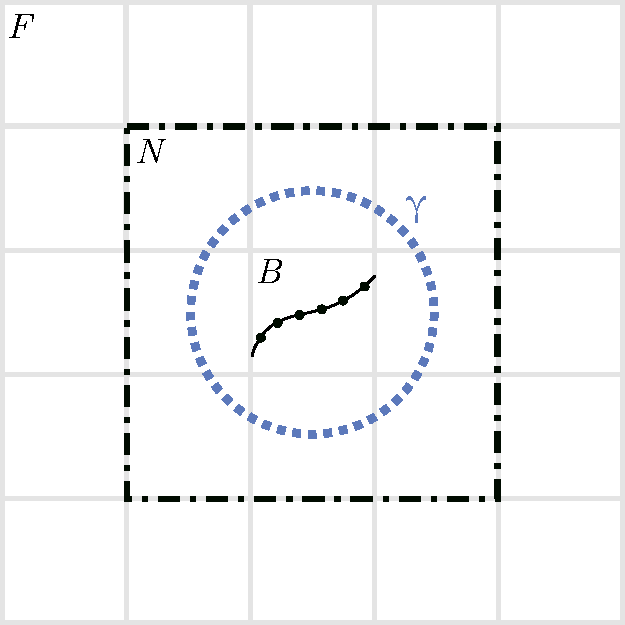
\includegraphics[width=0.5\textwidth]{ch_3/proxy.pdf}
    \caption{Considering the outgoing problem due to charge contained on $\Gamma \cap B$ evaluated in the far-field of $B$ in $\mathbb{R}^2$.}
    \label{fig:sec_3_1:proxy_trick}
\end{figure}

We can choose to represent our solution due to the charge in $B$ in $\mathcal{F}$ however we wish. However, our choice will lead to different matrices that we must compress.

Generally, we'll end up with a solution matrix of the form $A_{\mathcal{F}B}$ that maps between the charge contained $B$, $\psi_B$, and potential, $v_\mathcal{F}$, at points in its far-field that can be split up as,

\begin{flalign}
    v_{\mathcal{F}} &= A_{\mathcal{F}B} \psi_B \\
    &= B_{\mathcal{F}\gamma} C_{\gamma B} \psi_B
\end{flalign}

the subscripts indicate the domains these operators map between. We desire a split like this as the far field interaction of $B$ can be expressed as an object involving $C_{\gamma B}$ only.

To see how such a split can be useful consider the fact that $A_{\mathcal{F}B}$ can be written as,

\begin{flalign}
    \label{eq:decomposition}
    A_{\mathcal{F}B} = \begin{bmatrix}
        A_{\mathcal{Q}B}\\ A_{\mathcal{P}B}
        \end{bmatrix} = \begin{bmatrix}
        I & 0\\ 0 & B_{\mathcal{P}\gamma}
        \end{bmatrix} \begin{bmatrix}
        A_{\mathcal{Q}B}\\ C_{\gamma B}
        \end{bmatrix}
\end{flalign}

Our RS-S algorithm relies on a compression of this matrix, however as we noted a direct compression of $A_{\mathcal{F} B}$ is too expensive. However if we can find a decomposition like above, we can apply an interpolative decomposition to the right column in (\ref{eq:decomposition}) which has dimensions $O(1) \times O(n_\gamma)$ by construction where $n_\gamma$ is the number of proxy points. To prove that this allows us to reconstruct the full matrix after compression. Consider an ID that gives us,

\begin{flalign}
    \begin{bmatrix}
        A_{\mathcal{Q}B}\\ C_{\gamma B}
        \end{bmatrix} = \begin{bmatrix}
            A_{\mathcal{Q}S}\\ C_{\gamma S}
        \end{bmatrix} \begin{bmatrix}T_{SR}  & 1 \end{bmatrix}
\end{flalign}

Where $S$ and $R$ are the skeleton and redundant points respectively. Plugging back into our expression (\ref{eq:decomposition}),

\begin{flalign}
    \label{eq:compressed}
    A_{\mathcal{F}B} &=
        \begin{bmatrix}
            I & 0\\ 0 & B_{\mathcal{P}\gamma}
        \end{bmatrix}
        \begin{bmatrix}
             A_{\mathcal{Q}S}\\ C_{\gamma S}
        \end{bmatrix}
        \begin{bmatrix}T_{SR}  & 1 \end{bmatrix} \\
        &=\begin{bmatrix}
            A_{\mathcal{Q}S}\\ B_{\mathcal{P} \gamma}C_{\gamma S}
       \end{bmatrix} \begin{bmatrix}T_{SR}  & 1 \end{bmatrix} \\
       &=  A_{\mathcal{F}S} \begin{bmatrix}T_{SR}  & 1 \end{bmatrix}
\end{flalign}

Therefore, we see that we can get away with a cheap ID to reconstruct the far-field operator, involving the proxy points rather than the full far field of $B$. We are thus left with the task of formulating the proxy trick to compress the correct components of the boundary integral kernel.

Below we consider how to apply the proxy trick for different representations of the far-field potential due to the charges contained in $B$, known as `outgoing skeletonisations', as well the inverse operation in which the proxy trick is applied to calculate the potentials within $B$ due to charges in its far-field, known as `incoming skeletonisations'.

\subsubsection*{Hypersingular - $\mathcal{T}$}

\subsubsection*{Outgoing Skeletonisation}

A double-layer potential, due to some unknown density $\psi$, supported on $\tau$,

\begin{flalign}
    v(x) = \int_{\Gamma \cap B} \frac{\partial \Phi(x, y)}{\partial n(y)} \psi(y) ds(y) := \mathcal{D}\psi, \> \> x \in \mathbb{R}^m \setminus \tau
\end{flalign}

solves the Helmholtz equation everywhere it's valid. Here, $\Phi(x, y)$ is the fundamental solution of the Helmholtz equation. However, its normal derivative evaluated at the target points, known as the hypersingular operator, which we'll need for deriving boundary integral equations for Maxwell problems, does not,

\begin{flalign}
    \frac{\partial v}{\partial n(x)} = \frac{\partial}{\partial n(x)} \int_{\Gamma \cap B} \frac{\partial \Phi(x, y)}{\partial n(y)} \psi(y)ds(y) := \mathcal{T}\psi, \> \> x \in \Gamma \cap \mathcal{F}
\end{flalign}

it's only valid at far-field points, $\Gamma \cap \mathcal{F}$. However, we can separate out the normal part of the derivative,

\begin{flalign}
    \frac{\partial v}{\partial n(x)} = n(x) \cdot \nabla_x \int_{\Gamma \cap B} \frac{\partial \Phi(x, y)}{\partial n(y)} \psi(y)ds(y) := n \cdot w
\end{flalign}

The function

\begin{flalign}
    w(x) = \nabla_x \int_{\Gamma \cap B} \frac{\partial \Phi(x, y)}{\partial n(y)} \psi(y)ds(y) := \nabla_x \mathcal{D}\psi
\end{flalign}

Does satisfy our PDE, everywhere, and we'll exploit this fact in a moment. As an aside, we can see that this is true by considering a double layer potential $v$ that is smooth enough to admit,

\begin{flalign}
    (\Delta + k^2)w =(\Delta + k^2)\nabla_x v =\nabla_x (\Delta + k^2) v = 0
\end{flalign}

where the last equality follows as $v$ satisfies the Helmholtz equation. Therefore $w$ is a solution of the Helmholtz equation. Note that $w$ has three components.

In order to find our $C_{\gamma B}$ with this representation, we need to set up an `associated boundary value problem' for each component of $w$. The choice of boundary value problem we choose is free, as we only rely on the existence of its solution.

Consider an associated boundary value problem for just a single component of $\tilde{w}$ that satisfies,

\begin{flalign}
    &(\Delta + k^2)\tilde{w} = 0, \> \> x \in \mathbb{R}^m \setminus D \\
    &\tilde{w} = w_1(x) \\
    &\text{A radiation condition at } \infty
\end{flalign}

A combined field representation might be nice, as we know it has good properties,

\begin{flalign}
    \tilde{w} = (\mathcal{D} - ik \mathcal{S})_{\mathcal{F}\gamma} \mu
\end{flalign}

where $\mu$ is some unknown density supported on the proxy surface $\gamma$. Forming the boundary integral equation, and plugging back into the representation for $\tilde{w}$,

\begin{flalign}
    \tilde{w} &=  (\mathcal{D} - ik \mathcal{S})_{\mathcal{F} \gamma}(\frac{1}{2}\mathcal{I} + \mathcal{D} - ik \mathcal{S})_{\gamma \gamma}^{-1}w_1 \\
    &= (\mathcal{D} - ik \mathcal{S})_{\mathcal{F} \gamma}(\frac{1}{2}\mathcal{I} + \mathcal{D} - ik \mathcal{S})_{\gamma \gamma}^{-1} \nabla_1 \mathcal{D}_{\gamma B} \psi_\gamma \\
    &\equiv B_{\mathcal{F}\gamma} C_{\gamma B} \psi_\gamma
\end{flalign}

where we identify,

\begin{flalign}
    C_{\gamma B} = \nabla_1 \mathcal{D}_{\gamma B}
\end{flalign}

This is the matrix we will attempt to compress. Similar analysis follows for the other two components of $w(x)$. Meaning that we end up having to compress $[\nabla_1 \mathcal{D}_{\gamma B} , \nabla_2 \mathcal{D}_{\gamma B} , \nabla_3 \mathcal{D}_{\gamma B}]$ for the outgoing problem. We note that $B_{\mathcal{F} \gamma }$ is never explicitly formed, we just require its existence. When we calculate an approximation of $A_{\mathcal{F}B}$ using (\ref{eq:compressed}), we only need to know the ID of the $C_{\gamma B}$.

\subsubsection*{Incoming Skeletonisation}

For the incoming skeletonization, were again we're considering the same representation with a hypersingular operator, we observe that we're just looking for,

\begin{flalign}
    \left [\frac{\partial v}{\partial n(x)} \right ]_{\mathcal{F} B}^T
\end{flalign}

with the formation of an associated boundary integral equation taking place in much the same way as for the outgoing problem. However, the hypersingular operator is self-adjoint, therefore it leads to the same expressions for $C_{\gamma B}$.

\subsubsection*{Derivative of the Single Layer - $\mathcal{K}'$}

\subsubsection*{Outgoing Skeletonisation}

If we choose to represent our potential with a single-layer potential,

\begin{flalign}
    u(x) = \int_{\Gamma \cap B} \Phi(x, y) \phi(y) ds(y) := \mathcal{S}\phi, \> \> x \in \mathbb{R}^m \setminus \tau
\end{flalign}

and seek a boundary integral equation in terms of its normal derivative at the targets,

\begin{flalign}
    w(x) = \int_{\Gamma \cap B} \frac{\partial \Phi(x, y)}{\partial n(x)} \phi(y) ds(y) := \mathcal{K}'\phi, \> \> x \in \Gamma \cap \mathcal{F}
\end{flalign}

We observe the same problem as in the $\mathcal{T}$ case, where this expression is not a general solution of our PDE. We can similarly separate out the normal component and write,

\begin{flalign}
    \tilde{w}(x) := \int_{\Gamma \cap B} \nabla_x \Phi(x, y) \phi(y) ds(y), \> \> x \in \mathbb{R}^m \setminus \tau
\end{flalign}

Using the previous analysis for $\mathcal{T}$, we immediately recognise that the components we must compress are $C_{\gamma B} = \nabla_1 \mathcal{S}_{\gamma B}$, giving us $[\nabla_1 \mathcal{S}_{\gamma B}, \nabla_2 \mathcal{S}_{\gamma B}, \nabla_3 \mathcal{S}_{\gamma B}]$ to compress in total for the outgoing problem.

\subsubsection*{Incoming Skeletonisation}

Noticing that,

\begin{flalign}
    \left [\frac{\partial u}{\partial n(x)} \right ]_{\mathcal{F} B}^T = \int_{\Gamma \cap B} \frac{\partial \Phi(x, y)}{\partial n(y)} \phi(y) ds(y) = \mathcal{D}_{\gamma B} \phi
\end{flalign}

already satisfies our PDE without any further work, we can simply use it as our Dirichlet data in the associated boundary value problem. The matrix to compress being $C_{\gamma B} = \mathcal{D}_{\gamma B}$.

\subsubsection*{Single Layer - $\mathcal{S}$}

\subsubsection*{Outgoing Skeletonisation}

We now choose to represent our scattered solution with a single-layer operator,

\begin{flalign}
    u(x) =\int_{\Gamma \cap B} \Phi(x, y)\phi(y)ds(y) := \mathcal{S}\phi,\> \> x \in \mathbb{R}^m \setminus \tau
\end{flalign}

This satisfies the underlying PDE everywhere. We can now set up an associated exterior boundary value problem as before, and use our single-layer potential as Dirichlet boundary data.

\begin{flalign}
    (\Delta + k^2)w= 0, \> \> x \in \mathbb{R}^m \setminus D \\
    w = \mathcal{S}\phi, \> \> \text{on } \gamma \\
    \text{Radiation condition at }\infty
\end{flalign}

where $\phi$ is some unknown density supported on $\tau$. As before, we can form a boundary integral equation for this associated problem, and solve, recognising that the matrix to compress $C_{\gamma B} = \mathcal{S}_{\gamma B}$

\subsubsection*{Incoming Skeletonisation}

The single-layer operator is self-adjoint, leading to the same operator to compress. Spelling this out, consider the associated interior boundary value problem,

\begin{flalign}
    (\Delta + k^2)w= 0\> \> \text{in } D \\
    w = \mathcal{S}\phi \> \> \text{on } \gamma
\end{flalign}

The solution of an interior Helmholtz scattering problem may not be unique, but this doesn't matter for our purposes. Proxy compression doesn't require uniqueness, only existence. Let's seek a solution in the form of a combined-layer potential,

\begin{flalign}
    w(x) = (\mathcal{D}_\gamma - ik \mathcal{S}_\gamma)[\phi](x)
\end{flalign}

where the subscripts make it clear that the density is supported on $\gamma$. Forming the boundary integral equation,

\begin{flalign}
    (-\frac{\mathcal{I}}{2} + \mathcal{D}_\gamma - ik \mathcal{S}_\gamma)[\phi](x) = \mathcal{S}_{\mathcal{F} \gamma}[\phi](x)
\end{flalign}

Solving with the representation gives,

\begin{flalign}
    w = \mathcal{S}_{B \gamma}(-\frac{\mathcal{I}}{2} + \mathcal{D}_\gamma - ik \mathcal{S}_\gamma)^{-1}\mathcal{S}_{\gamma \mathcal{F}}[\phi](x) = C_{B \gamma}B_{\gamma \mathcal{F}}
\end{flalign}

where we recognize the matrix to compress as $C_{B\gamma} = \mathcal{S}_{B\gamma}$ in our proxy framework.

\subsection*{Double Layer - $\mathcal{D}$}

\subsubsection*{Outgoing Skeletonisation}

A double-layer potential, due to some unknown density $\psi$, supported on $\tau$,

\begin{flalign}
    v(x) = \int_{\Gamma \cap B} \frac{\partial \Phi(x, y)}{\partial n(y)} \psi(y) ds(y) := \mathcal{D}\psi, \> \> x \in \mathbb{R}^m \setminus \tau
\end{flalign}

solves the Helmholtz equation everywhere it's valid. Therefore it can be used as Dirichlet data for the associated boundary value problem for the outgoing skeletonization. Applying similar analysis to above, we identify the kernel to compress as $C_{\gamma B} = \mathcal{D}_{\gamma B}$.

\subsubsection*{Incoming Skeletonisation}

We notice that the transpose of the double layer operator is,

\begin{flalign}
    [u]^T_{\mathcal{F}B}(x) = \int_{\Gamma \cap B} \frac{\partial \Phi(x,y)}{\partial n(x)}\phi(y)ds(y)= \mathcal{K}'_{\gamma B}\phi
\end{flalign}

This in general does not satisfy our PDE everywhere, we again separate out the normal component, and as before, recognise that the components to compress are $[\nabla_1 \mathcal{S}_{\gamma B}, \nabla_2 \mathcal{S}_{\gamma B}, \nabla_2 \mathcal{S}_{\gamma B}]$.

\subsection*{Acoustic Sound Hard Scattering}

Let's now apply our fast direct solver framework, with proxy compression to some example problems. We begin with acoustic sound-hard scattering, which is a didactic example. Consider a scattered field $u^s$, that scatters off an object $\Omega$ and satisfies the Helmholtz equation in the exterior,

\begin{flalign}
    (\Delta + k^2)u^s = 0, \> \> \> \text{in  } \mathbb{R}^3 \setminus \Omega
\end{flalign}

The `sound hard' boundary condition on the surfae $\Gamma$ is
\begin{flalign}
    \frac{\partial u^s}{\partial n} = \frac{\partial u^{i}}{\partial n}, \> \> \> \text{in  } \Gamma
\end{flalign}

where $u^i$ is the incident wave. Using the analysis in \cite{Bruno2012}, we write down a `regularised' representation formula for our solution. This regularisation can be shown to have better spectral properties.

\begin{flalign}
    u^s =(\mathcal{K}_k \circ \mathcal{S}_K - i\eta \mathcal{S}_k)
\end{flalign}

where $k$ and $K$ are complex wave numbers, that may not be the same. We can take the trace of this representation, and its normal derivative at the targets, and find a boundary integral equation for the exterior problem,

\begin{flalign}
    (\frac{i \eta}{2} \mathcal{I}- i \eta \mathcal{K}'_k + \mathcal{T}_k \circ \mathcal{S}_K )\mu = g
\end{flalign}

using the Calder\'{o}n identity,

\begin{flalign}
    \mathcal{T}_k\circ \mathcal{S}_k = -\frac{1}{4}\mathcal{I} + \mathcal({K}_k')^2
\end{flalign}

which is true for any $k$, we arrive at a boundary integral equation,

\begin{flalign}
    \left ( i \eta(\frac{1}{2}\mathcal{I}  - \mathcal{K}'_k) - \frac{1}{4}I+ \mathcal({K}_k')^2 \right ) \mu = g
\end{flalign}

by defining $\theta := \mathcal{K}'_k \mu$, we can write the boundary integral equation as a system,

\begin{flalign}
\begin{pmatrix}
(\frac{i\eta}{2} - \frac{1}{4})\mathcal{I} - i \eta \mathcal{K}'_k & \mathcal{K}'_k  \\
 \mathcal{K}'_k & - \mathcal{I}
\end{pmatrix}
\begin{pmatrix} \mu \\ \theta \end{pmatrix} = \begin{pmatrix}
    g \\ 0
\end{pmatrix}
\end{flalign}

We can then place this system into our fast direct solver framework. Despite not knowing how to compress the system matrix altogether, we do know how to compress each block, as they each correspond to displacements of $\mathcal{K}'_k$.

Consider writing out our block matrix as,


\begin{flalign}
    \begin{pmatrix}
        A & B \\ C & D
    \end{pmatrix}
    \begin{pmatrix}
        \mu\\\theta
    \end{pmatrix}
   = \begin{pmatrix}
        g\\ 0
    \end{pmatrix}
\end{flalign}

and re-writing as,

\begin{flalign}
    \begin{pmatrix}
        \begin{pmatrix}
            A_{11} & B_{11} \\ C_{11} & D_{11}
        \end{pmatrix} & . & .\\
        . & . & \\
        . & &     \begin{pmatrix}
            A_{NN} & B_{NN} \\ C_{NN} & D_{NN}
        \end{pmatrix}
    \end{pmatrix}
    \begin{pmatrix}
        \mu_1 \\ \theta_1 \\ . \\ . \\ \mu_n \\ \theta_n
    \end{pmatrix} =
    \begin{pmatrix}
        g_1 \\ 0 \\ . \\ . \\ g_N \\ 0
    \end{pmatrix}
\end{flalign}

This system matrix remains numerically low-rank, and therefore can fit into our RS-S framework. Indeed, we now have to compress a system of matrix operators in order to capture its row space via the proxy trick.

\subsection*{Preliminary Numerical Experiments}

The paper on which we base our work \cite{sushnikova2022fmm} builds on the original RS-S algorithm \cite{minden2017recursive} by:

\begin{enumerate}
    \item Implementing generalized Gaussian quadratures for computing near-field interactions \cite{bremer2013numerical}.
    \item Determining a properly sampled discretisation of the proxy surface which depends on the box size in the octree, so as to sufficiently sample oscillatory kernels without oversampling.
    \item Handling the construction of the far-field partition into $\mathcal{F} = \mathcal{Q} \cup \mathcal{P}$
\end{enumerate}

We defer to to the original paper for a discussion of these aspects \cite{sushnikova2022fmm}. For our simulations we use these algorithms and quadrature rules as a black box in as implemented by the FMM3D-BIE software \cite{fmm3dbie}. To demonstrate the accuracy of the solver in light of our proxy trick formulation, we suppose that the sound hard condition is generated from a set of 50 test points placed at random locations on the surface of a test geometry, for which we choose the `wiggly torus' displayed in figure (\ref{fig:octree_example:sec_1_2}). The results of our solve are then compared to the potential expected from using a combined field representation at 50 random test locations in the exterior of the geometry.

\begin{flalign*}
    \text{error} = \frac{\sqrt{\sum_{j=1}^{50}|\tilde{u}(t_j)-u(t_j)|^2}}{\sqrt{\int_\Gamma|\sigma(x)|^2 da(x)}}
\end{flalign*}

where $\tilde{u}$ is our approximated potential, $u$ is the exact potential calculated from our test points, $t_j$, and $\sigma$ is the calculated charge density from the boundary integral equation. The torus is taken to be in a bounding box, each dimension of which is fixed at $1 \lambda$ where $\lambda$ is the wavelength of the incident wave, and we fix the error of the ID at $\epsilon = 5 \times 10^{-7}$, and the wavenumber $k=0.97$. Experiments are taken on a single-node of the Rusty Cluster at the Flatiron Institute, which consists of 240 28-core Intel Broadwell nodes with 512GB of RAM.

\begin{table}[h!]
    \centering
    \begin{tabular}{||c c c c c c c c||} 
        \hline
        $p$ & $N_{patch}$ & $N$  & $t_f$ (s) & $t_s$ (s)  & $t_q$ (s) & $m_f$ (GB) & $\epsilon$ \\ [0.5ex]
        \hline\hline
        4 & 50  & 750  & 0.8 & 0.03 & 0.8 & 0.04 & $4.7 \times 10^{-3}$ \\
        4 & 200 & 3000 & 6.6 & 0.08 & 1.4 & 0.6  & $3.3 \times 10^{-4}$ \\
        4 & 450 & 6750 & 84.9 & 0.2 & 2.5 & 2.9 & $5.2 \times 10^{-5}$ \\
        4 & 800 & 12000 & 324.9 & 0.6 & 4.2 & 7.5 & $1.6 \times 10^{-5}$ \\
        4 & 1250 & 18750 & 1138.8 & 1.1 & 6.2 & 15.2 & $5.8 \times 10^{-6}$ \\
        4 & 1800 & 27000 & 1839.7 & 1.7 & 8.8 & 25.2 & $2.4 \times 10^{-6}$ \\
        4 & 2450 & 36750 & 3322.6 & 2.4 & 11.8 & 41.1 & $1.2 \times 10^{-6}$ \\
        \hline
    \end{tabular}
    \caption{We measure the $L^2$ error with respect to the density  ($\epsilon$), time for solution ($t_s$), factorisation ($t_f$), quadrature computation ($t_q$) and memory required for factorisation ($m_f$) as a function of quadrature expansion order ($p$) and number of patches used to discretise the geometry ($N_{patch}$).}
    \label{table:sec_3_2:sh}
\end{table}


From table (\ref{table:sec_3_2:sh}), we observe linear scaling for $t_f$. However we observe sub-linear scaling for for $m_f$ and $t_s$, the authors of \cite{sushnikova2022fmm} suggest that this is due to the fixed wavenumber for increasing $N$. Meaning that the additional degrees of freedom introduced beyond a certain sampling in points per wavelength are more easily compressed. In order to make further observations about the convergence rate of our method more data is required, for higher order quadratures. We note that amount of memory used, even for the modest problem sizes tested, can be quite considerable. With our experiment where the number of quadrature points $N=36750$ consuming over 40GB of memory. This demonstrates the main trade-off of fast direct solvers in comparisons to iterative solvers.

\subsection*{Exposing Parallelism}

The RS-S algorithm exposes natural parallelism. Consider figure (\ref{fig:sec_3_1:rss_parallel}) which shows a four-colouring for a non-adaptive octree in $\mathbb{R}^2$ for simplicity, each colour can be independently skeletonised as skeletonisation only updates matrix entries corresponding to a box's near field. The same logic can be applied to the adaptive case, as well as the $\mathbb{R}^3$ case, albeit with more colours. As of writing there are no parallel implementations of the RS-S algorithms available as open-source packages.

\begin{figure}
    \centering
    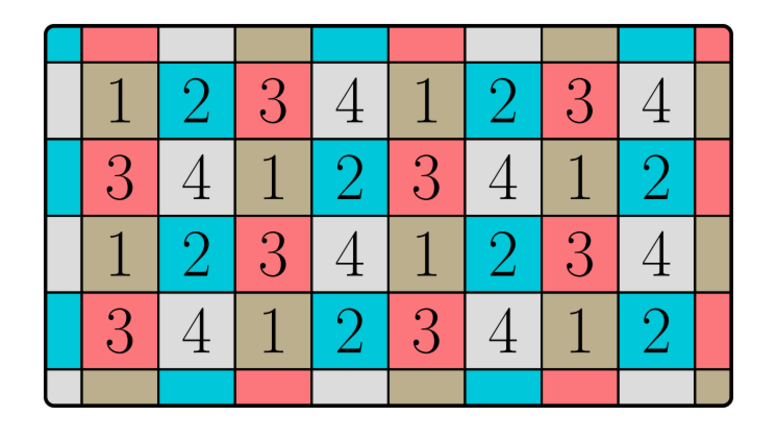
\includegraphics[width=0.5\textwidth]{ch_3/rss-parallel.pdf}
    \caption{A four-colouring of a non-adaptive quadtree in $\mathbb{R}^2$, where the colouring is chosen such that no box shares a colour with its neighbours. All boxes of a given colour can then be skeletonised independently. This figure is adapted from \cite{minden2017recursive}.}
    \label{fig:sec_3_1:rss_parallel}
\end{figure}

\subsection*{Conclusion}

We've described a scalar fast direct solver for solving acoustic scattering problems. We've demonstrated the convergence and scaling of our method with some preliminary numerical results, however further numerical testing is required to study the solvers properties. Specifically to understand its convergence behaviour, and scaling behaviour with higher order quadratures. We have only done cursory work on investigating the effect of quadrature choice, as well as the method chosen for sampling the proxy surface, using the default generalized Gaussian quadratures and sampling techniques described in \cite{sushnikova2022fmm}. This is another potential vector of research. The extension of this solver, and proxy formulation, to the full vectorial case which would allow us to tackle electromagnetic scattering problems as described by Maxwell's equations is an ongoing are of investigation.
    \chapter{Conclusion}\label{chpt:conclusion}

In this subsidiary thesis we've presented progress on the development of a new software infrastructure for fast algorithms. We've documented recent outputs towards this goal including foundational software as well as a algorithmic techniques. The main outputs being an investigation into programming languages and environments most suitable for scientific computing, a parallel load balanced octree library designed for high-performance,  as well as a proxy-compression based fast direct solver for acoustic Helmholtz scattering problems.

The immediate next steps of this project will be to publish our recent software results on octrees in an appropriate scientific journal. We also intend to continue the developments on fast direct solvers for oscillatory problems, and extend the RS-S framework to electromagnetic scattering problems described by Maxwell's equations. This would constitute a first fast direct solver for electromagnetic scattering problems. In the medium term, we plan to complete the implementation of the parallel FMM software, and the apply this to large scale boundary integral equation problems. This would entail the completion of the majority of our fast solver infrastructure. The final stage of this project will be the extension of our infrastructure to a parallel fast direct solver, and the simulation of large scale electromagnetic scattering problems.

    \appendix
    
\chapter{Deriving Local Expansion Coefficents from Multipole Expansion in $\mathbb{R}^2$}\label{app:locals}
Working in the setting in which we derived the multipole expansion in equation (\ref{eq:ch_2:multipole_expansions}),

\begin{flalign}
    \phi(x) = \sum_{j \in I_s} K(x, y)q_j = \log(x-c_s)\hat{q}_0^s + \sum_{p=1}^\infty \frac{1}{(x-c_s)^p}\hat{q}_p^s
    \label{eq:app:multipole_expansion}
\end{flalign}

Deriving the local expansion centered around the origin, where the bounding box of the targets, $\Omega_t$, is well separated from the source box, $\Omega_s$,

\begin{flalign*}
    \phi(x) = \sum_{l=0}^\infty \hat{\phi}^t_l (x-c_t)^l
\end{flalign*}

from the multipole expansion relies on the following expressions,

\begin{flalign*}
\log((x-c_t)-c_s) &= \log(-c_s(1-\frac{x-c_t}{c_s})) \\
&= \log(-c_s)  - \sum_{l=1}^\infty \frac{1}{l} \left( \frac{x-c_t}{c_s} \right) ^l
\end{flalign*}

and,


\begin{flalign*}
    ((x-c_t)-c_s)^{-p} &= \left( \frac{-1}{c_s} \right)^p \left( \frac{1}{1-\frac{x-c_t}{c_s}} \right)^p \\
    &=  \left( \frac{-1}{c_s} \right)^p \sum_{l=0}^\infty \binom{l+p-1}{p-1} \left( \frac{x-c_t}{c_s} \right)^l
\end{flalign*}

Substituting these expressions into (\ref{eq:app:multipole_expansion}), translated to be centred on $\Omega_t$

\begin{flalign*}
    \phi(x) &= \log((x-c_t)-c_s)\hat{q}^s_0 + \sum_{p=1}^\infty \frac{1}{((x-c_t)-c_s)^p}\hat{q}_p^s \\
     &= \log(-c_s)\hat{q}^s_0 - \left( \sum_{l=1}^\infty \frac{1}{l} \left( \frac{x-c_t}{c_s} \right) ^l\right) \hat{q}^s_0 + \sum_{p=1}^\infty \left( \frac{-1}{c_s} \right)^p \sum_{l=0}^\infty \binom{l+p-1}{p-1} \left( \frac{x-c_t}{c_s} \right)^l \hat{q}^s_p
\end{flalign*}

Identifying the local expansion coefficients as,

\begin{flalign*}
    \hat{\phi}^t_0 = \hat{q}^s_0 \log(-c_s) + \sum_{p=1}^\infty \frac{\hat{q}^s_p}{c_s^p}(-1)^p
\end{flalign*}

and,

\begin{flalign*}
    \hat{\phi}_l^t = \frac{-\hat{q}_0^s}{l c_s^l} + \frac{1}{c_s^l}\sum_{p=1}^\infty \frac{\hat{q}_p^s}{c_s^p} \binom{l+p-1}{p-1} (-1)^p
\end{flalign*}


\chapter{Hyksort}\label{app:hyksort}
The parallel splitter selection and HykSort algorithms are provided below. In terms of complexity analysis, we adapt the analysis provided in section 3.4 of \cite{sundar2013hyksort}. The main costs of SampleSort is sorting the splitters and the MPI collectives for data reshuffling. This can lead to a load imbalance and network congestion, represented by a constant $c$ below,

\begin{flalign*}
    T_{ss} = t_c c \frac{N}{p} \log \frac{N}{p} + (t_s + t_w p) \log^2 p + t_w c \frac{N}{p}
\end{flalign*}

Where $t_c$ is the intranode memory slowness (1/RAM bandwidth), $t_s$ interconnect latency, $t_w$ is the interconnect slowness (1/bandwidth), $p$ is the number of MPI tasks in $comm$, and $N$ is the total number of keys in an input array $A$, of length $N$.

The parallel splitter selection algorithm for determining $k$ splitters uses MPI collectives, \texttt{All\_Gather}() and \texttt{All\_Reduce}(). The main cost is in determining the local ranks of the samples using a binary search. The number of iterations $\eta$ depends on the input distribution, the required tolerance $N_\epsilon/N$ and the parameter $\beta$. The expected value of $\eta$ varies as $\log(\epsilon)/\log(\beta)$ and $\beta$ is chosen experimentally to minimise the running time, leading to a complexity of,

\begin{flalign*}
    T_{ps} = \eta t_c \beta k \log \frac{N}{p} + \eta (t_s + t_w \beta k) \log p
\end{flalign*}

HykSort relies on a specialised \texttt{All\_to\_all\_kway}() collective, we defer to the original paper for details. It uses only point to point communications with staged message sends and receives, allowing HykSort to minimise network congestion. It has $\log p / \log k$ stages with $O(N/p)$ data transfer and $k$ messages for each task in every stage. This leads to a complexity of,

\begin{flalign*}
    T_{a2a} = \left( t_s k + t_w \frac{N}{p} \right) \frac{\log p}{\log k}
\end{flalign*}

Finally, HykSort has the same communication pattern as \texttt{All\_to\_all\_kway}(). In addition it relies on the parallel splitter selection algorithm to determine splitters. The main computational cost is the initial local sort, and merging $k$ arrays during each iteration.

\begin{flalign}
    T_{Hk} = t_c \frac{N}{p} \log \frac{N}{p} + \left( t_c \frac{N}{p} + T_{ps}\right) \frac{\log p}{\log k} + T_{a2a}
\end{flalign}

Unlike SampleSort, the complexity of HykSort doesn't involve any $O(p)$ terms. This is the term that can lead to network congestion for higher core counts.

\begin{algorithm}
    \caption{\textbf{Parallel Select}}
    \begin{algorithmic}
        \STATE \textbf{Input:} $A_r$ - array to be sorted (local to each process), $n$ - number of elements in $A_r$, $N$ - total number of elements, $R[0,....,k-1]$ - expected global ranks, $N_\epsilon$ - global rank tolerance, $\beta \in [20, 40]$,

        \STATE \textbf{Output:} $S \subset A$ - global splitters, where $A$ is the global array to be sorted, with approximate global ranks $R[0,...,k-1]$

        \STATE $R^{\text{start}} \gets [0,...,0]$ - Start range of sampling splitters
        \STATE $R^{\text{end}} \gets [n,...,n]$ - End range of sampling splitters
        \STATE $n_s \gets [\beta/p,...,\beta/p]$ - Number of local samples, each splitters
        \STATE $N_{\text{err}} \gets N_\epsilon + 1$

        \WHILE{$N_{\text{err}} > N_\epsilon$}
            \STATE $Q' \gets A_r[\texttt{rand}(n_s, (R^{\text{start}}, R^{\text{end}}))]$
            \STATE $Q \gets$ \texttt{Sort}(\texttt{All\_Gather}($\hat{Q}'$))
            \STATE $R^{loc} \gets \texttt{Rank}(Q, A_r)$
            \STATE $R^{glb} \gets \texttt{All\_Reduce}(R^{loc})$
            \STATE $ I[i] \gets \text{argmin}_j | R^{glb} - R[I] | $
            \STATE $N_{err} \gets \max |R^{glb} - R{I}|$
            \STATE $R^{\text{start}} \gets R^{loc}[I-1]$
            \STATE $R^{\text{end}}  \gets R^{loc}[I+1]$
            \STATE $n_s \gets \beta \frac{R^{\text{end}}-R^{\text{start}}}{R^{glb}[I+1]-R^{glb}[I-1]}$
        \ENDWHILE
        \STATE \textbf{return }$S \gets Q[I]$
    \end{algorithmic}
\end{algorithm}

\begin{algorithm}
    \caption{\textbf{HykSort}}
    \begin{algorithmic}
        \STATE \textbf{Input:} $A_r$ - array to be sorted (local to each process), $comm$ - MPI communicator, $p$ - number of processes, $p_r$ - rank of current task in $comm$
        \STATE \textbf{Output:} globally sorted array $B$.
        \WHILE{$p > 1$, Iters: $O(\log p/\log k)$}
            \STATE $N \gets \texttt{MPI\_AllReduce}(|B|, comm)$
            \STATE $s \gets \texttt{ParallelSelect}(B, \{i N/k ; i=1,...,k-1 \})$
            \STATE $d_{i+1} \gets \texttt{Rank}(s_i, B), \> \forall i$
            \STATE $[d_0, d_k] \gets [0, n]$
            \STATE $color \gets \lfloor k p_r/p \rfloor$
            \PARFOR{ $i \in 0,...,k-1$}
                \STATE $p_{recv} \gets m((color-i)\text{mod}k)+(p_r \text{mod}m)$
                \STATE $R_i \gets \texttt{MPI\_Irecv}(p_{recv}, comm)$
            \ENDPARFOR

            \FOR{$i \in 0,...,k-1$}
                \STATE $p_{recv} \gets m((color-i)\text{mod}k)+p_r \text{mod}m$
                \STATE $p_{send} \gets m((color+i)\text{mod}k)+p_r \text{mod}m$
                \STATE $j \gets 2$
                \WHILE{$i > 0$ and $i \text{mod}j = 0$}
                    \STATE $R_{i-j} \gets \texttt{merge}(R_{i-j}, R_{i-j/2})$
                    \STATE $j \gets 2j$
                \ENDWHILE
                \STATE \texttt{MPI\_WaitRecv}($p_{recv}$)
            \ENDFOR
            \STATE \texttt{MPI\_WaitAll}()
            \STATE $B \gets \texttt{merge}(R_0, R_{k/2})$
            \STATE $comm \gets \texttt{MPI\_Comm\_splitt}($color, comm$)$
            \STATE $p_r \gets \texttt{MPI\_Comm\_rank}(comm)$
        \ENDWHILE
        \STATE \textbf{return } $B$
    \end{algorithmic}
\end{algorithm}

\chapter{Adaptive Fast Multipole Method Algorithm}\label{app:adaptive_fmm}
FMM literature distinguishes between types of relationships  between neighbouring nodes with the concept of \textit{interaction lists}. There are four such lists for a given node $B$, called $V$, $U$, $W$ and $X$. For a leaf node $B$, the $U$ list contains $B$ itself and leaf nodes adjacent to $B$. and the $W$ list consists of the descendants of $B$'s neighbours whose parents are adjacent to $B$. For non-leaf nodes, the $V$ list is the set of children of the neighbours of the parent of $B$ which are not adjacent to $B$, and the $X$ list consists of all nodes $A$ such that $B$ is in their $W$ lists. The non-adaptive algorithm is similar, however the $W$ and $X$ lists are empty

\begin{algorithm}
    \caption{\textbf{Adaptive Fast Multipole Method}.}
    \label{alg:fmm}
    \begin{algorithmic}

        \STATE $N$ is the total number of points
        \STATE $s$ is the maximum number of points in a leaf node.

        \STATE
        \STATE \textbf{Step 1: Tree construction}

        \FOR{each node $B$ in \textit{preorder} traversal of tree, i.e. the nodes are traversed bottom-up, level-by-level, beginning with the finest nodes.}
            \STATE subdivide $B$ if it contains more than $s$ points.
        \ENDFOR
        \FOR{each node $B$ in \textit{preorder} traversal of tree}
            \STATE construct \textit{interaction lists}, $U$, $V$, $X$, $W$
        \ENDFOR

        \STATE
        \STATE \textbf{Step 2: Upward Pass}
        \FOR{each leaf node $B$ in \textit{postorder} traversal of the tree, i.e. the nodes are traversed top-down, level-by-level, beginning with the coarsest nodes.}
        \STATE \textbf{P2M}: compute multipole expansion for the particles they contain.
        \ENDFOR
        \FOR{each non leaf node $B$ in \textit{postorder} traversal of the tree}
        \STATE \textbf{M2M}: form a multipole expansion by translating the expansion centre of its children to its centre and summing their multipole expansion coefficients.
        \ENDFOR

        \STATE
        \STATE \textbf{Step 3: Downward Pass}
        \FOR{each non-root node $B$ in \textit{preorder} traversal of the tree}
        \STATE \textbf{M2L}: translate multipole expansions of nodes in $B$'s $V$ list to a local expansion at $B$.
        \STATE \textbf{P2L}: translate the charges of particles in $B$'s $X$ to the local expansion at $B$.
        \STATE \textbf{L2L}: translate $B$'s local expansion to its children by translating its expansion centre to the centre of its children, and assigning the same coefficients.
        \ENDFOR

        \FOR{each leaf node $B$ in \textit{preorder} traversal of the tree}
        \STATE \textbf{P2P}: directly compute the local interactions using the kernel between the particles in $B$ and its $U$ list.
        \STATE \textbf{L2P}: translate local expansions for nodes in $B$'s $W$ list to the particles in $B$.
        \STATE \textbf{M2P}: translate the multipole expansions for nodes in $B$'s $W$ list to the particles in $B$.
        \ENDFOR
    \end{algorithmic}
    \end{algorithm}


    % \printglossary
    \printbibliography[heading=bibintoc]

\end{document}